% !TEX root = ../under-spec-z.tex

\documentclass[12pt]{article}





%%% Tools/essentials %%%

\usepackage[utf8]{inputenc}
\usepackage{embedfile}
\usepackage{enumerate}
\usepackage{mathtools}

\usepackage{tikz-cd}

\usepackage[left=1.5in, right=1.5in, top=1in, footskip=0.5in, bottom=1.2in]{geometry}




%%% Typography %%%

\usepackage{charter}
\usepackage{amsmath}
\usepackage{amssymb}
\usepackage{amsfonts}
\usepackage{mathrsfs}

\usepackage[T1]{fontenc}

\usepackage{fnpct}
\usepackage[symbol,perpage]{footmisc}

\usepackage[xspace]{ellipsis}

\renewcommand\labelitemi{{\boldmath$\cdot$}}

\usepackage{soul}
\newcommand{\ghl}[1]{{\sethlcolor{green}\hl{#1}}}
\newcommand{\rhl}[1]{{\sethlcolor{red}\hl{#1}}}

\usepackage{booktabs}
\usepackage{multirow}

\usepackage[font=footnotesize]{caption}





%%% Translation and commentary %%%

\makeatletter
\AtBeginEnvironment{mdframed}{%
\def\@fnsymbol#1{\ensuremath{\ifcase#1\or \dagger\or \ddagger\or
    \|\or **\or \dagger\dagger
   \or \ddagger\ddagger \else\@ctrerr\fi}}%
}   
\renewcommand\thempfootnote{\fnsymbol{mpfootnote}}
\makeatother

\newenvironment{translation}[2]
{%
    \par\noindent
    \vspace{0.4cm}%
    \begin{flushleft}%
        \marginpar{%
            \vspace{.6cm}\footnotesize\S\,#1\\\P\,#2%
        }%
        \begin{mdframed}%
            \textsf\bgroup\noindent\ignorespaces%%
}%
{%
            \noindent\ignorespacesafterend%
            \egroup%
        \hfill{\ensuremath{\blacksquare}}
        \end{mdframed}%
    \end{flushleft}%
    \vspace{0.4cm}%
}

\usepackage[%
linewidth=1pt,
linecolor=gray,
topline=true,
leftline=false,
rightline=true,
bottomline=false,
skipabove=0pt,
skipbelow=0pt,
innertopmargin=0.5cm,
leftmargin=0pt,
innerleftmargin=0pt,
rightmargin=-0.5cm,
innerrightmargin=0.5cm,
innerbottommargin=0.1cm,
]{mdframed}





%%% Titles, headers, and footers %%%

\usepackage{titlesec}

\usepackage{needspace}

% !TEX root = ../under-spec-z.tex

\titlespacing*{\section}
{0pt}{10.5ex plus 1ex minus .2ex}{5.3ex plus .2ex}
\titlespacing*{\subsection}
{0pt}{5.5ex plus 1ex minus .2ex}{4.3ex plus .2ex}
\titlespacing*{\subsubsection}
{0pt}{3.5ex plus 1ex minus .2ex}{2.3ex plus .2ex}

\titleformat*{\section}{\needspace{2in}\centering\huge\sffamily}
\titleformat*{\subsection}{\needspace{2in}\Large\sffamily}
\titleformat*{\subsubsection}{\needspace{2in}\large\sffamily}


\usepackage{fancyhdr}
\usepackage{lastpage}

\makeatletter
\newcommand{\resetHeadWidth}{\fancy@setoffs}
\makeatother

\fancypagestyle{pagenumbers}{%
  \fancyhf{}%
  \fancyfoot[C]{{\thepage ~of \pageref{LastPage}}}
}

\renewcommand{\headrulewidth}{0pt}





%%% Table of contents %%%

\usepackage{multicol}
% \usepackage[toc]{multitoc}
\usepackage{tocloft}

\makeatletter
\renewcommand{\@cftmaketoctitle}{}
\makeatother

\renewcommand{\cftdot}{}
\renewcommand{\cftpnumalign}{r}

% \renewcommand{\cftsecleader}{\quad}
\renewcommand{\cftsecafterpnum}{\cftparfillskip}
\renewcommand{\cftsecpagefont}{\bfseries\itshape}
\setlength{\cftbeforesecskip}{1em}

% \renewcommand{\cftsubsecleader}{\quad}
\renewcommand{\cftsubsecafterpnum}{\cftparfillskip}
\renewcommand{\cftsubsecpagefont}{\itshape}
\cftsetindents{subsection}{1em}{2.4em}
\setlength{\cftbeforesecskip}{.5em}

\renewcommand{\cftsubsubsecafterpnum}{\cftparfillskip}
\renewcommand{\cftsubsubsecpagefont}{\itshape}
\renewcommand{\cftsubsubsecaftersnumb}{\itshape}
\cftsetindents{subsubsection}{2em}{3.4em}
\setlength{\cftbeforesecskip}{.5em}





%%% Citations %%%

\usepackage[backend=biber,defernumbers=true,bibencoding=ascii,style=alphabetic,maxbibnames=99,maxalphanames=5]{biblatex}
\addbibresource{under-spec-z.bib}

\let\cite\autocite

\nocite{*}





%%% Theorem environments %%%

\usepackage{amsthm}
\usepackage{thmtools}
\usepackage{thm-restate}

% \usepackage[pdfpagelabels]{hyperref}
\usepackage[noabbrev,nameinlink,capitalize]{cleveref}

\usepackage{chngcntr}
\counterwithin{table}{section}

% !TEX root = ../under-spec-z.tex

\numberwithin{equation}{subsubsection}

\declaretheoremstyle[
    spacebelow=2\topsep,
    spaceabove=2\topsep,
    headfont=\normalfont\bfseries,
    bodyfont=\itshape,
    postheadspace=\newline,
    qed=${\lrcorner}$,
    headpunct={},
    notebraces={[}{]}
]{breakit}

\declaretheoremstyle[
    spacebelow=2\topsep,
    spaceabove=2\topsep,
    headfont=\normalfont\bfseries,
    bodyfont=\normalfont,
    postheadspace=\newline,
    qed=${\lrcorner}$,
    headpunct={},
    notebraces={[}{]}
]{breakup}

\declaretheorem[numberlike=equation,style=breakit]{theorem}
\declaretheorem[numberlike=theorem,style=breakit]{lemma}
\declaretheorem[numberlike=theorem,style=breakit]{corollary}

\declaretheorem[numberlike=theorem,style=breakup]{definition}
\declaretheorem[numberlike=theorem,style=breakup]{example}
\declaretheorem[numberlike=theorem,style=breakup]{note}

\numberwithin{theorem}{subsubsection}
\numberwithin{lemma}{subsubsection}
\numberwithin{corollary}{subsubsection}

\numberwithin{definition}{subsubsection}
\numberwithin{example}{subsubsection}
\numberwithin{note}{subsubsection}






%%% Appendices %%%

\usepackage{appendix}
\crefname{appsec}{Appendix}{Appendices}





%%% Notes to self %%%

\usepackage{environ}
\NewEnviron{fix}{\marginpar{\textcolor{magenta}{\BODY$\rightarrow$}}}


% !TEX root = ../under-spec-z.tex

\newcommand*\elide{\,\textup{[\,\dots]}\,}

\newcommand{\hookdoubleheadrightarrow}{%
  \hookrightarrow\mathrel{\mspace{-15mu}}\rightarrow
}

\DeclareMathSymbol{\mlq}{\mathord}{operators}{``}
\DeclareMathSymbol{\mrq}{\mathord}{operators}{`'}

\newcommand{\numberincircle}[1]{\raisebox{.5pt}{\textcircled{\raisebox{.2pt}{\tiny #1}}}}


\DeclareMathOperator{\spec}{Spec}
\DeclareMathOperator{\Hom}{Hom}
\DeclareMathOperator{\colim}{colim}
\DeclareMathOperator{\id}{id}
\DeclareMathOperator{\coeq}{coeq}
\DeclareMathOperator{\eq}{eq}
\DeclareMathOperator{\essim}{essim}
% \DeclareMathOperator{\Sch}{Sch}
% \DeclareMathOperator{\PShv}{PSh}
% \DeclareMathOperator{\Shv}{Sh}
% \DeclareMathOperator{\Fun}{Fun}
\newcommand{\Sch}{\mathsf{Sch}}
\newcommand{\ASch}{\mathsf{AffSch}}
\newcommand{\PShv}{\mathsf{PSh}}
\newcommand{\Shv}{\mathsf{Sh}}
\newcommand{\Fun}{\mathsf{Fun}}
\newcommand{\Loc}{\mathsf{Loc}}
\newcommand{\Fra}{\mathsf{Fra}}
\newcommand{\Ban}{\mathsf{Ban}}


\DeclareMathOperator{\GL}{GL}

\newcommand{\uHom}{\underline{\Hom}}

\newcommand{\nn}{\mathbb{N}}
\newcommand{\zz}{\mathbb{Z}}
\newcommand{\rr}{\mathbb{R}}
\newcommand{\cc}{\mathbb{C}}
\newcommand{\ff}{\mathbb{F}}
\newcommand{\dd}{\mathbb{D}}
\newcommand{\GG}{\mathbb{G}}

\newcommand{\smc}{(\mathcal{C},\otimes,1)}
\newcommand{\smd}{(\mathcal{D},\otimes,1)}
\newcommand{\ccat}{\mathcal{C}}
\newcommand{\dcat}{\mathcal{D}}
\newcommand{\tcat}{\mathcal{D}}
\newcommand{\ecat}{\mathcal{E}}

\newcommand{\commk}{\mathsf{CommAlg}_k}
\newcommand{\Cat}{\mathsf{Cat}}
\newcommand{\Set}{\mathsf{Set}}
\newcommand{\Ab}{\mathsf{Ab}}
\newcommand{\Grp}{\mathsf{Grp}}
\newcommand{\CRing}{\mathsf{CRing}}
\newcommand{\CSemiring}{\mathsf{CSemiring}}
\newcommand{\CMon}{\mathsf{CMon}}

\newcommand{\modc}[1]{{{#1}\hbox{-}\mathsf{Mod}}}
\newcommand{\algc}[1]{{{#1}\hbox{-}\mathsf{CommAlg}}}
\newcommand{\comm}[1]{\mathsf{Comm}\left({#1}\right)}
\newcommand{\schc}[1]{{#1}\hbox{-}\mathsf{Sch}}
\newcommand{\aff}[1]{\mathsf{Aff}_{#1}}
\newcommand{\Sp}[1]{\mathsf{Sp}_{#1}}
\newcommand{\Op}[1]{\mathsf{Op}(#1)}
\newcommand{\Zar}[1]{\mathsf{Zar}(#1)}
\newcommand{\AffZar}[1]{\mathsf{AffZar}(#1)}

\newcommand{\op}[1]{{#1}^{\mathrm{op}}}

\newcommand{\blank}{{-}}
\newcommand{\singleton}{\{*\}}

\newcommand{\nt}{\Rightarrow}
\newcommand{\congto}{\overset{\sim}{\longrightarrow}}

\newcommand{\famofmor}{\{p_i\colon X_i\to X\}_{i\in I}}

\newcommand{\tightunderset}[2]{\underset{\makebox[0pt]{\text{\footnotesize {#1}}}}{#2}}
\newcommand{\tightoverset}[2]{\overset{\makebox[0pt]{\text{\footnotesize {#1}}}}{#2}}


\title{Under $\spec\zz$\\ \Large{\textit{A reader's companion}}}
\author{Timothy Hosgood}

%%% Document %%%

\begin{document}

    \embedfile{\jobname.tex}

    %%% Title %%%

    % !TEX root = ../under-spec-z.tex

\begin{titlepage}
    \date{}
    \maketitle
    \vspace{-1em}
    \centering\large
%    Word Count: 9968\\[4em]

    \textit{Submitted as a}\\[0.3em]
    {\sc Part C Dissertation (COD)}\\[0.3em]
    \textit{for the}\\[0.3em]
    {\sc Final Honour School of Mathematics}\\[4em]

    University of Oxford\\
    Hilary Term 2016\\[4em]

    
\includegraphics[width=4cm]{images/ox_brand_cmyk_rev.eps}

    \thispagestyle{empty}
\end{titlepage}


    %%% Abstract and thanks %%%

    \pagestyle{pagenumbers}
    \setcounter{page}{1}
    
    % !TEX root = ../under-spec-z.tex

\begin{abstract}
    Relative algebraic geometry is an approach to algebraic geometry using category theory.
    This allows us to generalise algebraic geometry to many different settings.
    This project will cover basic notions from category theory, symmetric monoidal categories, Grothendieck topologies, algebraic geometry relative to a symmetric monoidal category and the example of classical algebraic geometry and monoid algebraic geometry which is a version of the field with one element.

    One very important paper in this area is \cite{Toen:2005wxa}, which is written in French, and translating the first few sections of it into English would open this paper up to a whole new audience.
    Although mathematical French is in general not entirely impenetrable when one is armed with a good dictionary or glossary, a lot of the language found in this paper is hard to find in other sources.
    Further, when we are dealing with such abstract mathematics, grammar and semantics are of the utmost importance, and small variations can change the meaning wildly, making `on-the-fly' translation tricky.

    The aims of this project are: to translate the first few sections (those dealing with establishing the formalities of the subject) of \cite{Toen:2005wxa} into English; to provide ample editorial commentary concerning the translation and historical context; and to comment on the mathematics in the paper, providing enough background information for the new reader to be able to follow the main ideas -- the main emphasis is placed on this last point.
\end{abstract}

    
    % \vfill

    \begin{figure}[h!]
        \centering
        \begin{minipage}[t]{0.45\textwidth}
            \vspace{0pt}
            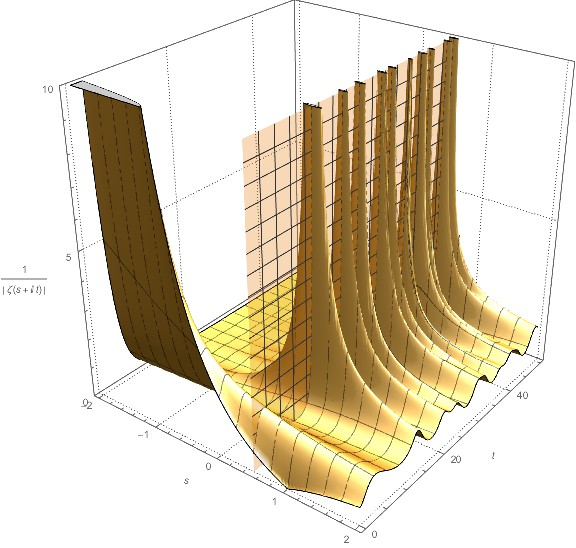
\includegraphics[width=\textwidth]{images/riemann-zeta.jpg}
        \end{minipage}
        \hfill
        \begin{minipage}[t]{0.53\textwidth}
            \vspace{0pt}
            \footnotesize
            \centering\textbf{Thanks}\\[.7em]
            \raggedright
            \begin{verse}
                \emph{Many thanks to give;}\\
                \emph{word limit too tight -- I swim}\\
                \emph{in deep gratitude.}
            \end{verse}
            Firstly, thanks to \cite{Lan:2012tj} for creating such an invaluable mathematical French dictionary.
            Secondly, thanks to Kobi Kremnitzer and Christopher Hollings for their excellent supervision, and for not complaining about the vast number of questions I asked.
            Lastly, thanks to all my family and friends, without whom I would not be lucky enough to be at university, let alone be able write this dissertation.
        \end{minipage}
    \end{figure}

    \begin{quotation}
        \footnotesize\emph{Point n'est besoin d'espérer pour entreprendre, ni de réussir pour perséverer}\\
        \raggedleft -- Willem van Oranje Nassau
    \end{quotation}


    % \vspace{4em}

    %%% Table of contents %%%

    \clearpage

    % \newgeometry{left=.5in,right=.5in}

    % \section*{Contents}
    % \vspace{-1em}

    \begin{center}
        \textbf{Contents}
    \end{center}

    \tableofcontents

    % \restoregeometry


    %%% REVERSE MARGINPAR SIDE %%%

    \reversemarginpar



    %%% Content %%%

    %TC:group figure 0 0

    \clearpage
    % !TEX root = ../../../under-spec-z.tex

\section{Introduction} % (fold)
\label{sec:introduction}

    \subsection{Formatting} % (fold)
    \label{ssub:formatting}

        This paper consists of translated sections from \cite{Toen:2005wxa} as well as the author's own writing.
        The general layout and order tries to follow that of the original paper as much as possible, including section numbering and naming.

        Longer sections of translated text will be boxed, left aligned, sans serif, and ended with a small black square ($\blacksquare$).
        At the start of such sections there will also be a reference to the location of the source text.
        Shorter `quotations' will simply be in italics and referenced afterwards.
        Theorems (and definitions) that have been translated will not be boxed off or in quotes, but there will be a reference to the original theorem (or definition) after the theorem (or definition) number.
        Hopefully it will be largely self-explanatory, but here are a few guidelines that the author has tried to adhere to:
        \begin{itemize}
            \item Usually they will be given as a section and a paragraph, e.g. (\S1\,\P2), where the paragraphs are counted by looking at indentations.
            \item Negative paragraph numbers indicate counting from the end of the section (as given), with the last paragraph being the -1st.
                For example, (\S2.1\,\P-2) would indicate the penultimate paragraph of section 2.1.
                (Luckily there are no subsubsections, so we don't have to worry about things getting any more complex.)
        \end{itemize}


        Sometimes a section that we wish to translate will contain some reference to a theorem or definition in the original paper, and this might have a different numbering in \emph{this} paper.
        Because of this, all such references (e.g. \emph{voir définition 2.12}) from the original will be suitably replaced with numbering relevant to \emph{this} paper (e.g. \emph{voir \elide (\cref{le:yoneda-lemma})}).

        If there are any references to a certain section or paragraph without specifying from which paper, then they are to \cite{Toen:2005wxa}.
        Similarly, if any lemma (or theorem) is stated without a proof then a proof can be found in the referenced lemma (or theorem) in \cite{Toen:2005wxa}.

        Finally, all footnotes, in translated sections or not, are by the author and \emph{not} from \cite{Toen:2005wxa}.


    \subsubsection{Conventions} % (fold)
    \label{ssub:conventions}

        We retain the following conventions from \cite{Toen:2005wxa}:
        \begin{translation}{1}{-2}
            All the monoids and monoidal categories considered will be unital and associative, and all modules over a monoid will be unital.
            We will ignore all set-theoretic problems to do with the choice of universe; the reader can consult \cite{Toen:2005er,Toen:2008wy} to find a method to resolve them.
        \end{translation}

        We also impose the following conventions ourselves, which are always assumed (unless otherwise stated):
        \begin{itemize}
            \item all algebras and rings are unital and associative;
            \item $k$ is an algebraically closed field;
            \item $0\in\nn$;
            \item for a ring $R$ we write $R^\times$ to mean the group of multiplicative units in $R$;
            \item $\GG_m=k^\times=k\setminus\{0\}$;
            \item for $n\in\nn\setminus\{0\}$ we write $\mu_n$ to mean the cyclic group of order $n$;
            \item given a category $\ccat$ we write $x\in\ccat$ to mean $x\in\mathrm{ob}(\ccat)$;
            \item `presheaf' means a $\Set$-valued presheaf.
        \end{itemize}
        We usually use `functor' to mean `covariant functor'.
        % It is not a strict convention, but we tend to think of functors as being covariant (and hence contravariant functors are functors from the opposite category).
        % This is not a universal view though, and some papers don't adopt this tendency, but the context should always make it clear how we are thinking about functors.

    % subsubsection conventions (end)


    % !TEX root = ../../../under-spec-z.tex

\subsection{Overview} % (fold)
\label{sub:overview}

    In this paper we will summarise some of the results of \cite{Toen:2005wxa}, providing background definitions along the way, as well as filling in some of the proofs that are omitted or only sketched.
    All of the pictures, as well as \cref{sub:background_knowledge,sec:further_applications}, are entirely original and aim to complement the main results (though the pictures are \emph{not} to be taken too literally -- they often illustrate simple cases, such as when $\ccat=\Op{T}$).
    There are also explanations of motivation (e.g. \cref{sub:under_}) and historical notes (e.g. \cref{sub:the_riemann_hypothesis}) that are original.
    This is why this paper is subtitled `\emph{a readers' guide}', and not simply `\emph{a translation}'.

    The results of \cite{Toen:2005wxa} are many, and we will not have time to cover most of the later sections;  we will focus largely on the first three\footnote{
        Not including the introduction, so sections 2 (\emph{Géométrie algébrique relative}), 3 (\emph{Trois exemples de géométries relatives}), and 4 (\emph{Quelques exemples de schémas au-dessous de $\spec\zz$}).
    } sections.
    Because of this, for us, the introduction of \cite{Toen:2005wxa} summarises the purpose of the paper better than the abstract.

    \vspace{-1em}

    \begin{translation}{1}{1}
        The aim of this paper is to construct several categories of \emph{schemes} that are defined over bases found \emph{under $\spec\zz$}.
        Of course, since $\zz$ is the initial object in the category of commutative rings, it is vital to leave the usual framework of rings and permit the use of more general objects, but only objects that  resemble commutative rings enough such that the notion of a scheme can still be defined.
        Our approach to this problem is based on the theory of relative algebraic geometry, largely inspired by \cite{Hakim:XPnOZC1P}.
        It comes from remarking that a commutative ring is nothing but a commutative monoid in the monoidal category of $\zz$-modules, and that, in general, for a symmetric monoidal category $\smc$, the commutative monoids in $\ccat$ can be thought of as models for the \emph{affine schemes relative to $\ccat$}.
        It is remarkable that such a general (simplistic, even) approach allows us to actually define the notion of schemes, and moreover in a functorial way in $\ccat$.
        So, in choosing $\ccat$ equipped with a sensible symmetric monoidal functor $\ccat\to\modc{\zz}$, we find a notion of schemes relative to $\ccat$ and a base-change functor to $\zz$-schemes, and thus a notion of schemes under $\spec\zz$.
        % In this paper we show how this approach, as well as its \ghl{homotopic generalisation where $\ccat$ is also equipped with a Quillen model structure}, allows us to define five categories of schemes found under $\spec\zz$.
    \end{translation}

% In this translation we mainly focus on section 2 (\emph{Relative algebraic geometry}), about which the introduction has the following to say.

% \begin{translation}{1}{2--5}
%     % The general ideas of relative algebraic geometry date back to \cite{Hakim:XPnOZC1P}, where \ghl{relative schemes over a ringed topos} are defined.
%     % In \cite{Deligne:2007hm} the case of schemes over a \ghl{tannakian category} is also considered.
%     The theory of relative  algebraic geometry that we present here is largely inspired by [\cite{Hakim:XPnOZC1P,Deligne:2007hm}], but considering categories over bases that aren't abelian, nor even additive, appears to be a novelty.
%     \\\\
%     Consider a symmetric monoidal category\footnote{
%         \cref{df:smc}
%     } $\smc$ that we also suppose to be complete, cocomplete, and closed\footnote{
%         Such a category is now often called a \emph{cosmos} (\cref{df:cosmos}).
%     } (i.e. possessing an internal $\Hom$ functor relative to the $\otimes$ monoidal structure).
%     It is well known\footnote{
%         Monoids, modules, and $\comm{\ccat}$ are all defined in \cref{ssub:preliminary_definitions}.
%         The change of base functor is discussed at length in \cref{ssub:change_of_base_for_modules_over_a_monoid}.
%     } that we have: the notion of a monoid in $\ccat$; for such a monoid $A$, the notion of a module; and for a morphism of monoids $A\to B$, a base-change functor $\blank\otimes_A B$ from $A$-modules to $B$-modules (see \cite{Saavedra:1972tn}).
%     In particular there exists the notion of commutative monoids (associative and unital) in $\ccat$, and they form a category that we call $\comm{\ccat}$.
%     We formally define the category of affine schemes relative to $\ccat$ by $\aff{\ccat}=\op{\comm{\ccat}}$.
%     \\\\
%     All of this is, for the moment, completely formal, but it produces a few miracles:
%     \begin{itemize}
%         \item There exists a natural Grothendieck topology on $\aff{\ccat}$ called the {\emph{flat topology}} \elide\footnote{
%             \cref{df:fpqc-topology,df:fpqc-zariski-covers}
%         }.
%         % The covering families $\{X_i\to X\}$ for this topology correspond to the \ghl{finite families of morphisms} $\{A\to A_i\}$ in $\comm{\ccat}$ such that the base-change functor \ghl{on} the category of modules
%         % $$\prod_i\left(\blank\otimes_A A_i\right): \modc{A} \longrightarrow \prod_i\left(\modc{A_i}\right)$$
%         % is exact and conservative.
        
%         \item The flat topology on $\aff{\ccat}$ so defined is subcanonical (i.e. representable presheaves are sheaves).

%         \item There exists the notion of \emph{Zariski open} in $\aff{\ccat}$ \elide\footnote{
%             \cref{df:zariski-open-morphism}
%         }.
%         % , and they are by definition the morphisms $f\colon X\to Y$ for which the corresponding morphism \mbox{$A\to B$} in $\comm{\ccat}$ satisfies the following three conditions:
%         % \begin{enumerate}
%         %     \item \textit{$f$ is a monomorphism:} for all $A'\in\comm{\ccat}$ the \ghl{induced} morphism $\Hom(B,A')\to\Hom(A,A')$ is injective;
            
%         %     \item \textit{$f$ is \ghl{flat}:} the base-change functor
%         %     $$(\blank\otimes_A B) \colon \modc{A} \longrightarrow \modc{B}$$
%         %     is exact;

%         %     \item \textit{$f$ is a finite presentation:} for all filtered diagrams of objects $C_i\in A/\comm{\ccat}$, the natural morphism
%         %     $$\colim\Hom_{A/\comm{\ccat}}(B,C_i) \longrightarrow \Hom_{A/\comm{\ccat}}(B,\colim C_i)$$
%         %     is bijective.
%         % \end{enumerate}

%         \item The notion of Zariski open extends naturally to general morphisms between sheaves (see \elide(\cref{df:zariski-open-sheaves})).

%         \item The Zariski-open morphisms are stable under composition, isomorphism\footnote{
%             That is, composition with an arbitrary isomorphism.
%         }, and change of base.

%         \item The Zariski-open morphisms give rise to a notion of a Zariski topology, and this is again subcanonical.
%     \end{itemize}
    
%     The above properties are all that we need to define a category of schemes relative to $\smc$.
%     Indeed, a relative scheme is by definition a sheaf on the site $\aff{\ccat}$, endowed with the Zariski topology, and possessing a Zariski-open cover by affine schemes (see \elide(\cref{df:relative-scheme})).
%     The categories of schemes thus obtained is denoted $\sch{\ccat}$.
%     It is a full subcategory, stable under pullbacks and disjoint unions, of the category of sheaves on $\aff{\ccat}$.
%     Further it contains a full subcategory of affine schemes, that are exactly the representable sheaves, and is naturally equivalent to the category $\comm{\ccat}$, opposite to the category of commutative monoids in $\ccat$ (see \elide(\cref{sub:the_faithfully_flat_topology})).
%     Finally, the purely categorical nature of the construction makes the category $\sch{\ccat}$ functorial in $\ccat$, at the very least for left symmetric-monoidal adjoints $\smc\to\smd$ satisfying certain (easy to verify in practice) conditions (see \elide(\cref{sub:changes_of_bases})).
% \end{translation}

% subsection overview (end)



    % !TEX root = ../../../under-spec-z.tex

\subsection{Background knowledge} % (fold)
\label{sub:background_knowledge}

    This section acts as a prelude to \cite{Toen:2005wxa}, containing a few motivating examples and prerequisite definitions and lemmas.
    Before diving straight into the abstract definitions, we give an example of why we might think to try a category-theoretic approach to algebraic geometry.

    \subsubsection{Motivating example} % (fold)
    \label{ssub:motivating_example}

        Let $A$ be a finitely-generated commutative $k$-algebra.
        Then we can write
        \begin{equation*}
            A=\frac{k[x_1,\ldots,x_n]}{(f_1,\ldots,f_m)}
        \end{equation*}
        for some $m,n\in\nn$ and $f_i\in k[x_1,\ldots,x_n]$.
        If $B$ is another commutative $k$-algebra (not necessarily finitely generated) then the collection of algebra morphisms $A\to B$ is in bijection with points of $B^n$ that vanish on all of the $f_i$, since a morphism is determined entirely by where it sends each of the $x_i$ whilst satisfying $0\mapsto0$.
        So, letting $\commk$ denote the category of commutative $k$-algebras,
        \begin{equation}\label{eq:link-between-hom-and-varieties}
            \Hom_{\commk}(A,B)\cong\{b\in B^n \mid f_1(b)=\ldots=f_m(b)=0\}
        \end{equation}
        where, as usual, we evaluate $f_i(b)$ inside $B$.

        \Cref{eq:link-between-hom-and-varieties} implies that we should maybe think of $\Hom(A,B)$ as some variety inside $B^n$ determined by $A$, for general $A,B\in\commk$, and so we might be able to recover a lot of algebraic geometry from studying these $\Hom(A,B)$.
        In fact, thinking of $\Hom(A,\blank)$ as a functor $\commk\to\Set$ which takes an algebra $B$ to a \emph{variety} (a set of points) inside $B^n$, we are led to the more general idea of studying \emph{all} functors $\commk\to\Set$, and calling such functors \emph{spaces}.

        Before formalising this, we first recall a few things from category theory.
        
        \begin{definition}[Presheaves]\label{df:presheaves}
            Let $\ccat$ be a category.
            The category of \emph{presheaves on $\ccat$} is defined as the functor category $\PShv(\ccat)=\Fun(\op{\ccat},\Set)$, whose objects are (covariant) functors $\op{\ccat}\to\Set$ and morphisms are natural transformations $F\nt G$ between such functors.
        \end{definition}

        % \begin{figure}[h]
        %     \centering
        %     \frame{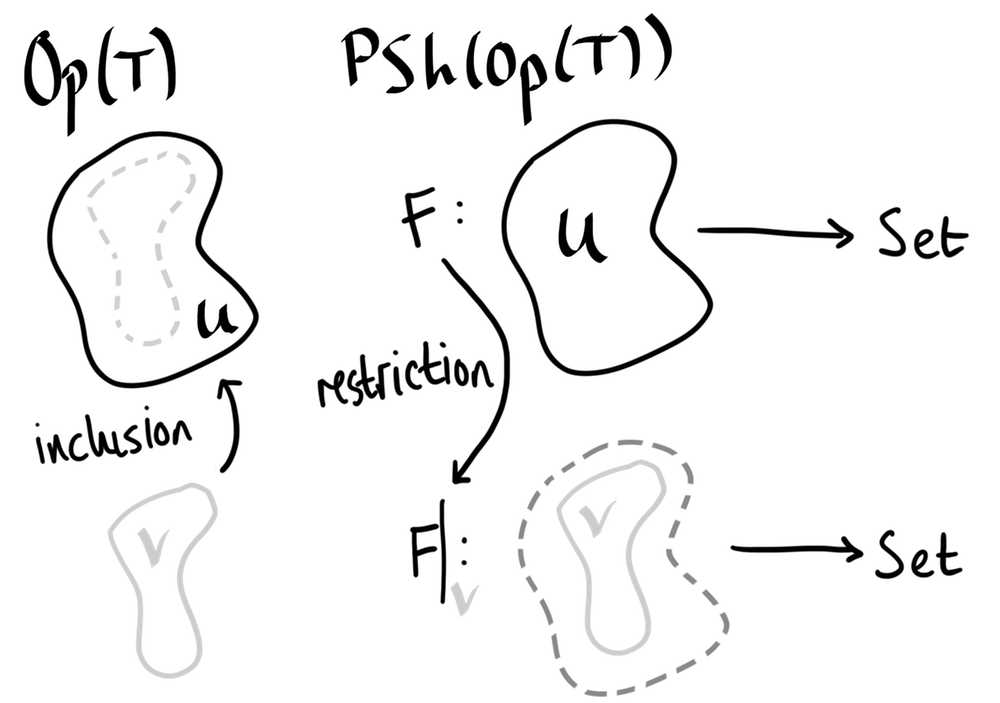
\includegraphics[width=.6\textwidth]{images/presheaves.png}}
        %     \caption{Presheaves on $\Op{T}$ (see paragraph after \cref{df:pullbacks}) -- inclusion of open sets corresponds to restriction of presheaves}
        %     \label{fg:presheaves}
        % \end{figure}

        \begin{figure}[h]
            \centering
            \frame{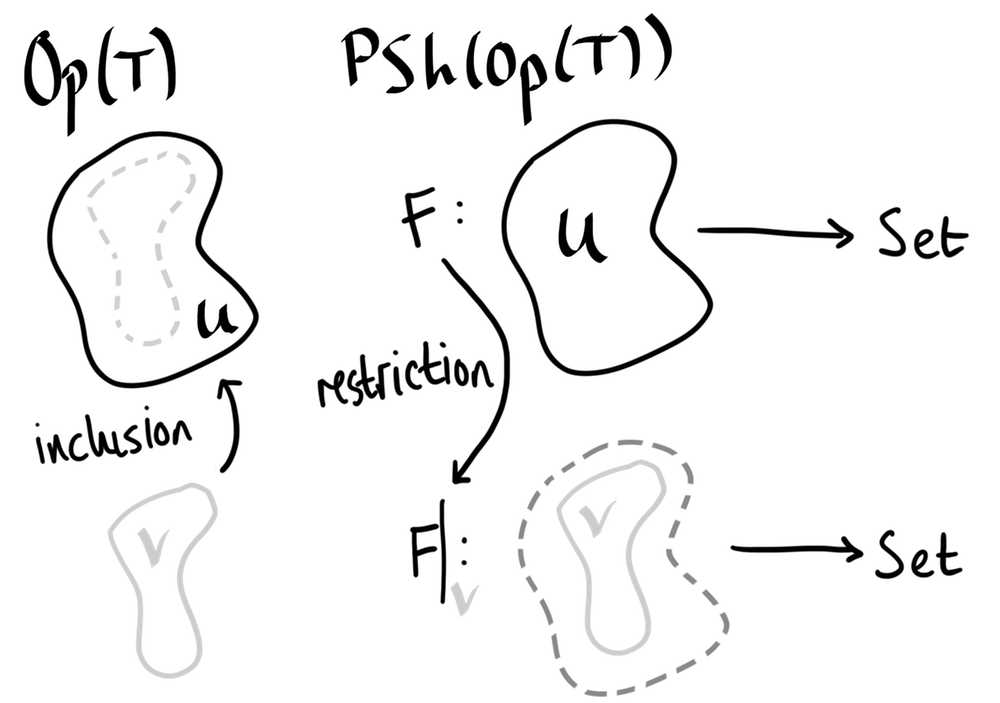
\includegraphics[width=.63\textwidth]{images/presheaves.png}}
            \caption{Presheaves on $\Op{T}$ (see paragraph after \cref{df:pullbacks}) -- inclusion of open sets corresponds to restriction of presheaves}\label{fg:presheaves}
        \end{figure}

        \begin{lemma}[Yoneda lemma]\label{le:yoneda-lemma}
            Let $\ccat$ be a locally small category\footnote{
                That is, the hom-sets $\Hom(A,B)$ are actual sets for all $A,B\in\ccat$.
            }.
            Define the \emph{downwards Yoneda functor}\footnote{
                This is not at all common terminology.
                It is often called the \emph{contravariant Yoneda functor}: it maps an object $A\in\ccat$ to the \emph{contravariant} functor $\Hom_\ccat(\blank,A)\colon\ccat\to\Set$.
                But the functor $\ccat\to\PShv(\ccat)$ itself is \emph{covariant}, so we use `downwards' to avoid confusion.
                The dual `covariant' (\emph{upwards}, in our terminology) functor is $Y^{(\blank)}\colon\op{\ccat}\to\Fun(\ccat,\Set)$ given by $\spec A\mapsto Y^A=\Hom_\ccat(A,\blank)$, where we write $\spec A\in\op{\ccat}$ to be the object corresponding to $A\in\ccat$.
                Then the statement $\Hom_{\Fun(\ccat,\Set)}(Y^A,G)\cong G(A)$ holds.
            } by
            \begin{align*}
                Y_{(\blank)}\colon&\ccat\to\PShv(\ccat)\\
                &A\mapsto \Hom_\ccat(\blank, A),
            \end{align*}
            which is well defined, since $\Hom(\blank, A)\colon\op{\ccat}\to\Set$ covariantly.
            Then, for any $A\in\ccat$ and $F\in\PShv(\ccat)$,
            \begin{equation}
                \Hom_{\PShv(\ccat)}(Y_A,F) \cong F(A)
            \end{equation}
            via the canonical restriction map.
            Further, $Y$ is fully faithful.
        \end{lemma}

        \begin{proof}
            See \cite[\S III.2, p.59--62]{Lane:1998fe}.
        \end{proof}

        Since $\commk$ is locally small\footnote{
            As in \cite{Toen:2005wxa}, we try to ignore such set-theoretic issues, but here we have the reasonable explanation that $\commk$ is a concrete category, and thus locally small.
        }, we can make the definitions in \cref{tb:comm-k-definitions}, where $Y$ is the Yoneda functor from \cref{le:yoneda-lemma}\footnote{
            In the definition of $\spec$ we use the fact that any covariant functor $F\colon\ccat\to\dcat$ induces a contravariant functor $F\colon\op{\ccat}\to\dcat$, and vice versa.
        }.
        
        \bigskip
        \begin{table}[h!]
            \centering
            \begin{tabular}{lcc}
                Name & Notation & Definition\\
                \toprule
                the category of \emph{affine schemes over $k$} & $\aff{k}$ & $\op{\commk}$\\
                the category of \emph{$k$-spaces} & $\Sp{k}$ & $\PShv(\aff{k})$\\
                the \emph{spectrum functor} & $\spec$ & $Y\colon\commk\to\Sp{k}$
            \end{tabular}
            \caption{Categorical approach to algebraic geometry with $\commk$}
            \label{tb:comm-k-definitions}
        \end{table}
        \bigskip

        We've already given a reason for calling objects of the functor category $\Fun(\commk,\Set)$ \emph{spaces}, and we call objects of $\op{\commk}$ \emph{schemes} because we know that the Yoneda lemma (\cref{le:yoneda-lemma}) will give us a way of viewing $\aff{k}$ as sitting inside of $\Sp{k}$.

        \begin{lemma}[Yoneda embedding]\label{le:yoneda-embedding}
            The category $\aff{k}$ is equivalent to the essential image of the Yoneda functor $Y\colon\aff{k}\to\Sp{k}$.
        \end{lemma}

        \begin{proof}
            Here we use the fact that a functor gives an equivalence of categories if and only if it is fully faithful and essentially surjective\footnote{
                \cite[Theorem~1, \S IV.4]{Lane:1998fe}
            }.
            \cref{le:yoneda-lemma} tells us that $Y$ is fully faithful so it forms an equivalence of categories between $\aff{k}$ and the essential image of $Y$ in $\Sp{k}$.
        \end{proof}

        So \cref{le:yoneda-embedding} lets us imagine $\aff{k}$ as sitting inside $\Sp{k}$.
        This mirrors classical algebraic geometry where, loosely speaking, given some commutative ring $R$ we define the space $\spec R$ of prime ideals of $R$ endowed with the Zariski topology.
        We can then give $\spec R$ some extra structure to make it an affine scheme.
        Then $\spec$ is a map taking commutative rings to affine schemes, which form a subclass of the objects (schemes) in which we're interested.

        Studying algebraic geometry this way is called the \emph{functor of points} approach\footnote{
            As opposed to the traditional \emph{ringed space} approach.
        }, because \cref{le:yoneda-embedding} says that describing some affine scheme $X\in\aff{k}$ is exactly the same as describing its functor of points $X(\blank)\in\Sp{k}$ under the Yoneda embedding.
        Sometimes this latter method is far easier, as the following example shows.

        \begin{example}[$\GL_n$]\label{ex:gln-affine-scheme}
            Given $A\in\commk$ we can define $\GL_n(A)$ to be the group of $n\times n$ invertible matrices over $A$.
            This induces a functor $\GL_n(\blank)\colon\op{\aff{k}}\to\Set$, so $\GL_n(\blank)\in\Sp{k}$.
            We claim that this functor is in the essential image of the Yoneda (spectrum) functor $Y\colon\commk\to\Sp{k}$, and is thus represented by an affine scheme.
            This is not obvious a priori.
            To prove this, we need to find an isomorphism
            \begin{equation*}
                \GL_n(\blank)\cong\Hom_{\commk}(R,\blank)=\spec R
            \end{equation*}
            for some $R\in\commk$, where we mean $\spec R$ as defined in \cref{tb:comm-k-definitions}\footnote{
                That is, identify $\spec R\in\aff{k}$ with $\spec R:=\Hom_{\op{\commk}}(\blank,R)$.
            }.
            By definition, this is equivalent to finding a bijection of sets $\GL_n(A)\cong\Hom_{\commk}(R,A)$ that transforms naturally in $A$ for each $A\in\commk$.

            Note that an element of $\GL_n(A)$ is a choice of $x_{11},x_{21},\ldots,x_{nn}\in A$ such that $\det(x_{ij})$ is invertible.
            That is, there exists some $y\in A$ such that $y\det(x_{ij})=1$.
            Hence
            \begin{equation*}
                R=\frac{k[x_{11},x_{21},\ldots,x_{nn},y]}{(y\det(x_{ij})-1)}
            \end{equation*}
            gives us the desired result, and so $GL_n=R\in\aff{k}$ is an affine scheme.
        \end{example}

    % subsubsection motivating_example (end)


    \subsubsection{Preliminary definitions} % (fold)
    \label{ssub:preliminary_definitions}

        We now give some definitions of which \cite{Toen:2005wxa} assumes prior knowledge.
        The motivation for them usually comes from taking $\ccat=\Set$, and their application to algebraic geometry can be better understood\footnote{
            Since \emph{\elide a commutative ring is nothing but a commutative monoid in the monoidal category of $\zz$-modules \elide} (\S1 p.2 \P1).
        } by taking $\ccat=\modc{\zz}=\Ab$.
        We assume that the reader is familiar with notions such as categories, functors, natural transformations, and functor categories, but not too much else.

        \begin{definition}[Monoidal category]\label{df:monoidal-category}
            A \emph{monoidal category} consists of the following data:
            \begin{itemize}
                \item a category $\ccat$;
                \item an object $1\in\ccat$, which we call the \emph{unit} or \emph{identity};
                \item a bifunctor $(\blank\otimes\blank)\colon\ccat\times\ccat\to\ccat$, called the \emph{monoidal} or \emph{tensor product};
                \item natural isomorphisms $\alpha$ (the \emph{associator}), $\lambda$ (the \emph{left unitor}), and $\rho$ (the \emph{right unitor}), constructed from morphisms
                \begin{equation*}
                    \begin{array}{rrcl}
                        \alpha_{ABC}\colon & (A\otimes B)\otimes C & \congto & A\otimes(B\otimes C)\\
                        \lambda_A\colon & 1\otimes A & \congto & A\\
                        \rho_A\colon & A\otimes1 & \congto & A
                    \end{array}
                \end{equation*}
                for all $A,B,C\in\ccat$.
            \end{itemize}
            Further, the three natural isomorphisms are subject to the following coherence conditions\footnote{
                These diagrams simply say that $\otimes$ is associative in all the ways that you might expect.
            }:
            \begin{itemize}
                \item (\emph{unit associativity}) for all $A,B\in\ccat$ the following commutes
                    \begin{equation*}
                        \begin{tikzcd}[row sep=3em]
                            (A\otimes 1)\otimes B \arrow[dr, swap, "\rho_A\otimes\id_B"] \arrow[rr, "\alpha_{A1B}"] & & A\otimes(1\otimes B) \arrow[dl, "\id_A\otimes\lambda_B"]\\
                             & A\otimes B &
                        \end{tikzcd}
                    \end{equation*}
                \item (\emph{4-associativity}) for all $A,B,C,D\in\ccat$ the following commutes
                    \begin{equation*}
                        \begin{tikzcd}[column sep=-3em, row sep=4em, cramped]
                            & (A\otimes(B\otimes C))\otimes D \arrow[rr, "\alpha_{A(B\otimes C)D}"] & & A\otimes((B\otimes C)\otimes D) \arrow[dr, "\id_A\otimes\alpha_{BCD}"] &\\
                            ((A\otimes B)\otimes C)\otimes D \arrow[ur, "\alpha_{ABC}\otimes\id_D"] \arrow[drr, "\alpha_{(A\otimes B)CD}", swap] & & & & A\otimes(B\otimes(C\otimes D)) \\
                             & & (A\otimes B)\otimes(C\otimes D) \arrow[urr, "\alpha_{AB(C\otimes D)}", swap] & &
                        \end{tikzcd}\qedhere
                    \end{equation*}
            \end{itemize}
        \end{definition}

        \begin{definition}[Symmetric monoidal category]\label{df:smc}
            A monoidal category $\smc$ is \emph{symmetric} if it can be equipped with a \emph{maximally-symmetric brading $\gamma$}.
            That is, for all $A,B\in\ccat$, there exists an isomorphism
            \begin{equation*}
                \gamma_{AB}\colon A\otimes B\congto B\otimes A
            \end{equation*}
            that is natural in both $A$ and $B$, and also subject to the following coherence conditions\footnote{
                These diagrams simply say that $\otimes$ is commutative in all the ways you might expect.
            }:
            \begin{itemize}
                \item (\emph{unit associativity}) for all $A\in\ccat$ the following commutes:
                    \begin{equation*}
                        \begin{tikzcd}
                            1\otimes A \arrow[rr, "\gamma_{1A}"] \arrow[dr, swap, "\lambda_A"] & & A\otimes 1 \arrow[dl, "\rho_A"]\\
                             & A &
                        \end{tikzcd}
                    \end{equation*}
                \item (\emph{3-associativity}) for all $A,B,C\in\ccat$ the following commutes:
                    \begin{equation*}
                        \begin{tikzcd}[column sep=4em,row sep=3em]
                            (A\otimes B)\otimes C \arrow[r, "\gamma_{AB}\otimes\id_C"] \arrow[d, swap, "\alpha_{ABC}"] & (B\otimes A)\otimes C \arrow[d, "\alpha_{BAC}"]\\
                            A\otimes(B\otimes C) \arrow[d, swap, "\gamma_{A(B\otimes C)}"] & B\otimes(A\otimes C) \arrow[d, "\id_B\otimes\gamma_{AC}"]\\
                            (B\otimes C)\otimes A \arrow[r, "\alpha_{BCA}"] & B\otimes(C\otimes A)
                        \end{tikzcd}
                    \end{equation*}
                \item (\emph{maximal symmetry}) for all $A,B\in\ccat$ the following commutes:
                    \begin{equation*}
                        \begin{tikzcd}
                             & B\otimes A \arrow[dr, "\gamma_{BA}"] & \\
                            A\otimes B \arrow[ur, "\gamma_{AB}"] \arrow[rr, swap, "\id_{A\otimes B}"] & & A\otimes B
                        \end{tikzcd}
                    \end{equation*}\qedhere
            \end{itemize}
        \end{definition}

        \begin{definition}[Closed symmetric monoidal category\footnote{ See \cite[Hypothese 2.6,~p.14]{Toen:2005wxa}}]\label{df:closed-smc}
            A symmetric monoidal category $\smc$ is \emph{closed} if, for all $A\in\ccat$, the functor $\blank\otimes A\colon\ccat\to\ccat$ has a right adjoint, written $(A\nt\blank)$.
            This means that
            \begin{equation*}
                \Hom(X\otimes A,B)\cong\Hom(X,A\nt B)
            \end{equation*}
            naturally in $X$ and $B$ for all $A,B,X\in\ccat$.
            The object $(A\nt B)\in\ccat$ is called the \emph{internal Hom}\footnote{
                \cite{Toen:2005wxa} uses the notation $\uHom(A,B)$.
            }.
        \end{definition}

        \begin{lemma}
            Let $\smc$ be a closed symmetric monoidal category.
            Then the bifunctor
            \begin{equation*}
                (\blank\otimes\blank)\colon\ccat\times\ccat\to\ccat
            \end{equation*}
            commutes with colimits in both of its arguments.
        \end{lemma}

        \begin{proof}
            % \emph{(We first show commutativity only in the first argument, and then explain at the end how to use this to complete the proof.)}

            % Fix $A\in\ccat$ and let $\{X_i\}_{i\in I}$ be a collection of objects in $\ccat$.
            % Assume that we have some $B\in\ccat$ with morphisms $X_i\otimes A\to B$ for all $i\in I$, and such that
            % \begin{equation}\label{eq:colim-commute-setup}
            %     \begin{tikzcd}[column sep=2em]
            %         X_i\otimes A \arrow[dr] \arrow[rr] & & X_j\otimes A \arrow[dl]\\
            %          & B &
            %     \end{tikzcd}
            % \end{equation}
            % commutes for all $X_i\otimes A\to X_j\otimes A$.
            % Then we want to show that there exists
            % \begin{itemize}
            %     \item morphisms $X_i\otimes A,X_j\otimes A\to(\colim X_i)\otimes A$;
            %     \item a \emph{unique} morphism $(\colim X_i)\otimes A\to B$,
            % \end{itemize}
            % such that the following diagram commutes:
            % \begin{equation}\label{eq:what-we-want-to-commute}
            %     \begin{tikzcd}[column sep=1em,row sep=2em]
            %         X_i\otimes A \arrow[dr] \arrow[ddr, bend right] \arrow[rr] & & X_j\otimes A \arrow[dl] \arrow[ddl, bend left]\\
            %          & (\colim X_i)\otimes A \arrow[d] &\\
            %          & B &
            %     \end{tikzcd}
            % \end{equation}

            % If we can show this, then, because the colimit is unique up to unique isomorphism\footnote{
            %     We write $X\overset{!}{\cong}Y$ to mean there these exists a \emph{unique} isomorphism between $X$ and $Y$.
            % },
            % \begin{equation*}
            %     (\colim X_i)\otimes A\overset{!}{\cong} \colim(X_i\otimes A).
            % \end{equation*}

            % \bigskip

            % This proof is largely diagram chasing, and it's easy to get lost in notation, but the idea behind it is comparatively simple: we construct four \emph{unique} morphisms that make certain diagrams commute, then put them all together.

            % \begin{enumerate}[(i)]

            %     \item \emph{Universal property of $\colim(X_i\otimes A)$}:

            %         By definition, there exists a unique $\pi\colon\colim(X_i\otimes A)\to B$ such that
            %         \begin{equation*}
            %             \begin{tikzcd}[column sep=1em,row sep=2em]
            %                 X_i\otimes A \arrow[dr] \arrow[ddr, bend right] \arrow[rr] & & X_j\otimes A \arrow[dl] \arrow[ddl, bend left]\\
            %                  & \colim(X_i\otimes A) \arrow[d, "\pi"] &\\
            %                  & B &
            %             \end{tikzcd}
            %         \end{equation*}
            %         commutes.

            %     \item \emph{Closedness of $\smc$ and universal property of $\colim X_i$}:

            %         \Cref{df:closed-smc} tells us that there is an isomorphism
            %         \begin{equation*}
            %             \Hom(X_i\otimes A, B)\cong\Hom(X_i,A\nt B)
            %         \end{equation*}
            %         for all $i\in I$ that is natural in both $X_i$ and $B$.
            %         This naturality means exactly that the morphism $X_i\to (A\nt B)$ coming from our morphism $X_i\otimes A\to B$ in \cref{eq:colim-commute-setup} is such that
            %         \begin{equation*}
            %             \begin{tikzcd}[column sep=1em]
            %                 X_i \arrow[dr] \arrow[rr] & & X_j \arrow[dl]\\
            %                  & (A\nt B) &
            %             \end{tikzcd}
            %         \end{equation*}
            %         commutes for all $X_i\to X_j$.
            %         So, by definition, there exists a unique morphism $\varphi\colon\colim(X_i)\to(A\nt B)$ such that
            %         \begin{equation*}
            %             \begin{tikzcd}[column sep=1em,row sep=2em]
            %                 X_i \arrow[dr] \arrow[ddr, bend right] \arrow[rr] & & X_j \arrow[dl] \arrow[ddl, bend left]\\
            %                  & \colim X_i \arrow[d, "\varphi"] &\\
            %                  & (A\nt B) &
            %             \end{tikzcd}
            %         \end{equation*}
            %         commutes.

            %     \item \emph{Functoriality of $\blank\otimes A$}:

            %         Since $\blank\otimes A$ is a functor, it preserves composition of morphisms, and so
            %         \begin{equation*}
            %             \begin{tikzcd}[column sep=1em,row sep=2em]
            %                 X_i\otimes A \arrow[dr] \arrow[ddr, bend right] \arrow[rr] & & X_j\otimes A \arrow[dl] \arrow[ddl, bend left]\\
            %                  & (\colim X_i)\otimes A \arrow[d, "\varphi\otimes A"] &\\
            %                  & (A\nt B)\otimes A &
            %             \end{tikzcd}
            %         \end{equation*}
            %         also commutes.
            %         Further, the uniqueness of $\varphi$ ensures that $\varphi\otimes A$ is also unique.

            %     \item \emph{Universal property of $\colim(X_i\otimes A)$}:

            %         We are now in the situation of \cref{eq:colim-commute-setup}: there exists a unique morphism $\psi\colon\colim(X_i\otimes A)\to (A\nt B)\otimes A$ making the following diagram commute:
            %         \begin{equation*}
            %             \begin{tikzcd}[column sep=1em,row sep=2em]
            %                 X_i\otimes A \arrow[dr] \arrow[ddr, bend right] \arrow[rr] & & X_j\otimes A \arrow[dl] \arrow[ddl, bend left]\\
            %                  & \colim (X_i\otimes A) \arrow[d, "\psi"] &\\
            %                  & (A\nt B)\otimes A &
            %             \end{tikzcd}
            %         \end{equation*}

            %     \item \emph{Adjunction $(\blank\otimes A)\dashv(A\nt\blank)$}:

            %         The adjunction $(\blank\otimes A)\dashv(A\nt\blank)$ hands us a natural transformation (the \emph{counit}) $\varepsilon\colon(A\nt\blank)\otimes A\nt\id_{\ccat}$.
            %         On the level of objects, this gives us a morphism
            %         \begin{equation*}
            %             \varepsilon_B\colon(A\nt B)\otimes A\to B.
            %         \end{equation*}

            %     \item \emph{Putting it all together}:

            %         There exists the unique morphism $\pi\colon\colim(X_i\otimes A)\to B$, but the composition $\varepsilon_B\circ\psi$ has the same source and target.
            %         This tells us that $\pi=\varepsilon_B\circ\psi$, but $\psi$ exists and is unique.
            %         So $\varepsilon_B$ exists and is the unique morphism $(A\nt B)\otimes A\to B$.
            %         Finally then, $\varphi\otimes A\colon(\colim X_i)\otimes A\to(A\nt B)\otimes A$ exists and is unique.
            %         Thus
            %         \begin{equation*}
            %             \varepsilon_B\circ(\varphi\otimes A)\colon (\colim X_i)\otimes A\to B
            %         \end{equation*}
            %         exists, is unique, and makes \cref{eq:what-we-want-to-commute} commute.

            % \end{enumerate}

            % \bigskip
            Since $(\blank\otimes A)$ has a right adjoint, it commutes with colimits (see \cref{le:adjoint-and-commuting-with-limits}).
            This gives us commutativity in the first argument.
            As for commutativity in the second argument, we claim that
            \begin{equation*}
                A\otimes(\colim X_i) \overset{(1)}{\cong} (\colim X_i)\otimes A \overset{(2)}{\cong} \colim(X_i\otimes A) \overset{(3)}{\cong} \colim(A\otimes X_i).
            \end{equation*}
            \begin{enumerate}[(1)]
                \item follows since $\smc$ is symmetric;
                \item follows from our first statement;
                \item requires a bit of work, but using the isomorphisms $X_i\otimes A\cong A\otimes X_i$ and the fact that they are \emph{natural} in both $A$ and $X_i$ we can show that $\colim(X_i\otimes A)$ satisfies the universal property required to be the colimit of $\{A\otimes X_i\}$, giving us the required isomorphism.\qedhere
            \end{enumerate}
        \end{proof}

        \begin{definition}[Cosmos]\label{df:cosmos}
            A (\emph{Bénabou}\footnote{
                After the French mathematician Jean Bénabou.
            }) \emph{cosmos}\footnote{
                Possible etymology: \emph{catégorie monoïdale symétrique} gets initialised to \emph{CMS} which gets pronounced `acronymically' as \emph{cosmos}.
            } is a bicomplete\footnote{
                All small limits and small colimits exist.
            } closed symmetric monoidal category.
        \end{definition}

        \begin{definition}[Commutative monoid in $\smc$]\label{df:comm-c}
            A \emph{commutative monoid $(A,\mu,\eta)$} in a symmetric monoidal category $\smc$ is an object $A\in\ccat$ along with morphisms
            \begin{itemize}
                \item $\mu\colon A\otimes A\to A$ (\emph{multiplication});
                \item $\eta\colon1\to A$ (\emph{unit}),
            \end{itemize}
            such that the following commute:
            \begin{itemize}
                \item (\emph{associativity})
                    \begin{equation*}
                        \begin{tikzcd}[column sep=0.2em, row sep=3em, cramped]
                            & A\otimes(A\otimes A) \arrow[rr, "\id_A\otimes\mu"] & & A\otimes A \arrow[dr, "\mu"] &\\
                            (A\otimes A)\otimes A \arrow[ur, "\alpha_{AAA}"] \arrow[drr, "\mu\otimes\id_A", swap] & & & & A \\
                             & & A\otimes A \arrow[urr, "\mu", swap] & &
                        \end{tikzcd}
                    \end{equation*}
                \item (\emph{left and right unity})
                    \begin{equation*}
                        \begin{tikzcd}[column sep=3em, row sep=3em]
                            1\otimes A \arrow[r, "\eta\otimes\id_A"] \arrow[dr, swap, "\lambda_A"] & A\otimes A \arrow[d, "\mu"] & A\otimes1 \arrow[l, swap, "\id_A\otimes\eta"] \arrow[dl, "\rho_A"]\\
                             & A &
                        \end{tikzcd}
                    \end{equation*}
                \item (\emph{commutativity})
                    \begin{equation*}
                        \begin{tikzcd}
                            A\otimes A \arrow[rr, "\gamma_{AA}"] \arrow[dr, swap, "\mu"] & & A\otimes A \arrow[dl, "\mu"]\\
                             & A &
                        \end{tikzcd}
                    \end{equation*}
            \end{itemize}

            We denote the category of all such objects by $\comm{\ccat}$, where the morphisms are morphisms $f\colon A\to A'$ in $\ccat$ such that everything transfers nicely (that is, $\eta'=f\circ\eta\colon1\to A'$ and $f\circ\mu=\mu'\circ (f\otimes f)\colon A\otimes A\to B$).
        \end{definition}

        \begin{definition}[Module over a monoid]\label{df:module-over-monoid}
            Let $\smc$ be a symmetric monoidal category and $A\in\comm{\ccat}$ a commutative monoid in $\ccat$.
            A \emph{module\footnote{
                Really this is the definition for a \emph{left} $A$-module, but since $A$ is commutative the notions of right and left modules coincide.
            } $(M,\sigma)$ over $A$} is an object $M\in\ccat$ with a morphism $\sigma\colon A\otimes M\to M$ such that the following diagrams commute\footnote{
                That is, $\sigma$ is an \emph{action}.
            }:
            \begin{itemize}
                \item (\emph{compatibility with $\mu$})
                    \begin{equation*}
                        \begin{tikzcd}[row sep=4em, column sep=3em]
                            A\otimes A\otimes M \arrow[r, "\id_A\otimes\sigma"] \arrow[d, swap, "\mu\otimes\id_M"] & A\otimes M \arrow[d, "\sigma"]\\
                            A\otimes M \arrow[r, "\sigma"] & M
                        \end{tikzcd}
                    \end{equation*}
                \item (\emph{unity})
                    \begin{equation*}
                        \begin{tikzcd}[row sep=2em]
                            1\otimes M \arrow[rr, "\eta\otimes\id_M"] \arrow[dr, swap, "\lambda_M"] & & A\otimes M \arrow[dl, "\sigma"]\\
                             & M &
                        \end{tikzcd}
                    \end{equation*}
            \end{itemize}

            We denote the category of all such objects by $\modc{A}$, where the morphisms are morphisms $f\colon M\to M'$ in $\ccat$ such that everything transfers nicely (that is, $f\circ\sigma=\sigma'\circ(\id_A\otimes f)\colon A\otimes M\to M'$).
        \end{definition}

        % We don't really use the internal Hom of $\smc$, apart from to tell us that $\blank\otimes A$ is right exact, but there is an interesting point here about how it ties in with modules.
        % Specifying a morphism $\sigma\colon A\otimes M\to M$ is (by closedness) equivalent to specifying a morphism $\varphi\colon A\to(M\nt M)$.
        % Further, the axioms for $\sigma$ to be an action correspond to $\varphi$ being a monoid morphism (where $(M\nt M)$ is a monoid with composition as the binary operation, and identity $\id_M$).
        % So, if we wanted to, we could rephrase \cref{df:module-over-monoid} in terms of a module morphism $\varphi\colon A\to(M\nt M)$ instead of an action $\sigma\colon A\otimes M\to M$.

    % subsubsection preliminary_definitions (end)


% subsection background_knowledge (end)



% section introduction (end)

    \clearpage
    % !TEX root = ../../../under-spec-z.tex

\section{Relative algebraic geometry} % (fold)
\label{sec:relative_algebraic_geometry}

\vspace{-2em}
\begin{translation}{2}{1}
    The aim of this first part is to present the idea of a scheme relative to a symmetric monoidal category $\ccat$.
    We start with a general process of construction of Grothendieck topologies from prestacks in categories satisfying certain conditions.
    This allows us to then define the \emph{faithfully flat and quasi-compact topology}, as well as the \emph{Zariski topology} in the very general setting.
    We will afterwards define the idea of a relative scheme by gluing back together affine objects with the help of the Zariski topology.
\end{translation}
\vspace{-2em}

% !TEX root = ../../../under-spec-z.tex

\subsection{Constructing Grothendieck topologies} % (fold)
\label{sub:constructing_grothendieck_topologies}

    \subsubsection{Exactness and pullbacks} % (fold)
    \label{ssub:exactness_and_pullbacks}

        \begin{definition}[Conservative functor]
            Let $F\colon\ccat\to\dcat$ be a functor.
            Then $F$ is \emph{conservative} if, for all morphisms $f$ in $\ccat$, whenever the morphism $F(f)$ in $\dcat$ is an isomorphism then so too is $f$.
        \end{definition}

        \begin{definition}[Exact functor]
            Let $F$ be a functor.
            We say that $F$ is \emph{left exact} if it commutes with finite limits.
            Dually, $F$ is \emph{right exact} if it commutes with finite colimits.
            If $F$ is both left and right exact, then we say that it is \emph{exact}.
        \end{definition}

        If $F\colon\ccat\to\dcat$ where $\ccat$ and $\dcat$ both have zero objects then, loosely speaking, $F$ being conservative is saying that\footnote{
            If we wanted to really abuse notation then we would write this as $F^{-1}(0)=\{0\}$.
        } $[F(c)=0\implies c=0]$, and $F$ being exact is saying that $F(0)=0$.

        \begin{lemma}\label{le:adjoint-and-commuting-with-limits}
            Let $(F\dashv G)$ be an adjunction of functors.
            Then $F$ commutes with colimits and $G$ commutes with limits.
            % Let $F$ be some functor that has a left adjoint (or, equivalently, \emph{is} a right adjoint).
            % Then $F$ commutes with limits.
            % Dually, let $G$ be some functor that has a right adjoint (or, equivalently, \emph{is} a left adjoint).
            % Then $G$ commutes with colimits.
        \end{lemma}

        \begin{proof}
            \cite[\S V.5, p.118]{Lane:1998fe}
        \end{proof}

        \begin{corollary}\label{co:adjoint-exactness}
            Left-adjoint functors are right exact; right-adjoint functors are left exact.
        \end{corollary}

        \begin{definition}[Pullbacks]\label{df:pullbacks}
            Let $\ccat$ be a category, $X,X',Y\in\ccat$ objects, and $f\colon X\to Y$, $g\colon X'\to Y$ morphisms:
            \begin{equation*}
                \begin{tikzcd}[row sep=.7em]
                    X \arrow[dr, "f"] &\\
                     & Y\\
                    X' \arrow[ur, swap, "g"] &
                \end{tikzcd}
            \end{equation*}
            Then the \emph{pullback} (or \emph{fibred product}) \emph{of $Y$ (along $f$ and $g$)} is the limit of this diagram (if it exists) and is written as $X\prescript{f}{}{\times}^g_Y X'$ (or just $X\times_Y X'$ when no confusion may arise).
            The commutative diagram
            \begin{equation*}
                \begin{tikzcd}[row sep=.7em]
                     & X \arrow[dr, "f"] &\\
                    X\times_Y X' \arrow[ur, "\pi_X"] \arrow[dr, swap, "\pi_{X'}"] & & Y\\
                     & X' \arrow[ur, swap, "g"] &
                \end{tikzcd}
            \end{equation*}
            is also called a \emph{cartesian square}.
        \end{definition}

        Since the pullback is a limit, if our category $\ccat$ has finite limits then it has pullbacks.
        In $\Set$, the pullback $X\times_A Y$ is given by `intersecting' the images of $X$ and $Y$ in $A$:
        \begin{equation*}
            X\times_A Y = \{(x,y)\in X\times Y\mid f(x)=g(y)\}.
        \end{equation*}
        Working in $\Op{T}$ for some topological space $T$ -- the category whose objects are open sets of $T$ and whose morphisms are the inclusion maps of the open sets -- pullbacks correspond to intersections (\cref{fg:opTandpullbacks}).
        So pullbacks generalise intersection, but also \emph{fibres}: let $Y,T$ be topological spaces, $p\in T$ some point with inclusion map $\iota\colon \{p\}\hookrightarrow T$, and $f\colon Y\to T$ continuous.
        Then the pullback is the \emph{fibre} (or \emph{preimage}) \emph{of $p$ under $f$}:
        \begin{equation*}
            Y\times_T \{p\}=\{y\in Y\mid f(y)=p\}.
        \end{equation*}
        (\cref{fg:pullback-as-fibre}).
        So when we have a continuous $\tau\colon S\to T$ we can think of $Y\times_T S$ as the \emph{fibre of the points of $\tau(S)\subset T$ under $f$}.

        \begin{figure}[h]
            \centering
            \begin{minipage}{0.4\textwidth}
                \centering
                \frame{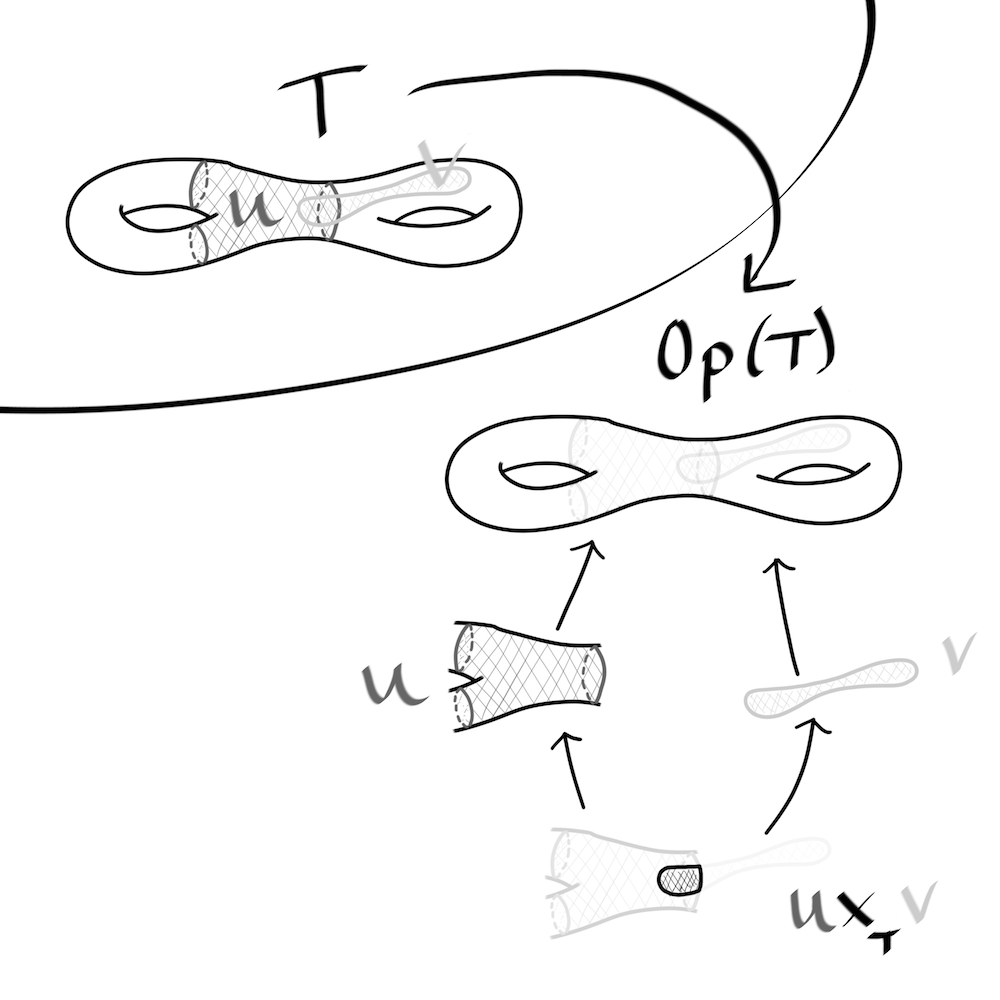
\includegraphics[width=\textwidth]{images/opTandpullbacks.png}}
                \caption{Pullbacks in $\Op{T}$}
                \label{fg:opTandpullbacks}
            \end{minipage}
            \hfill
            \begin{minipage}{0.59\textwidth}
                \centering
                \frame{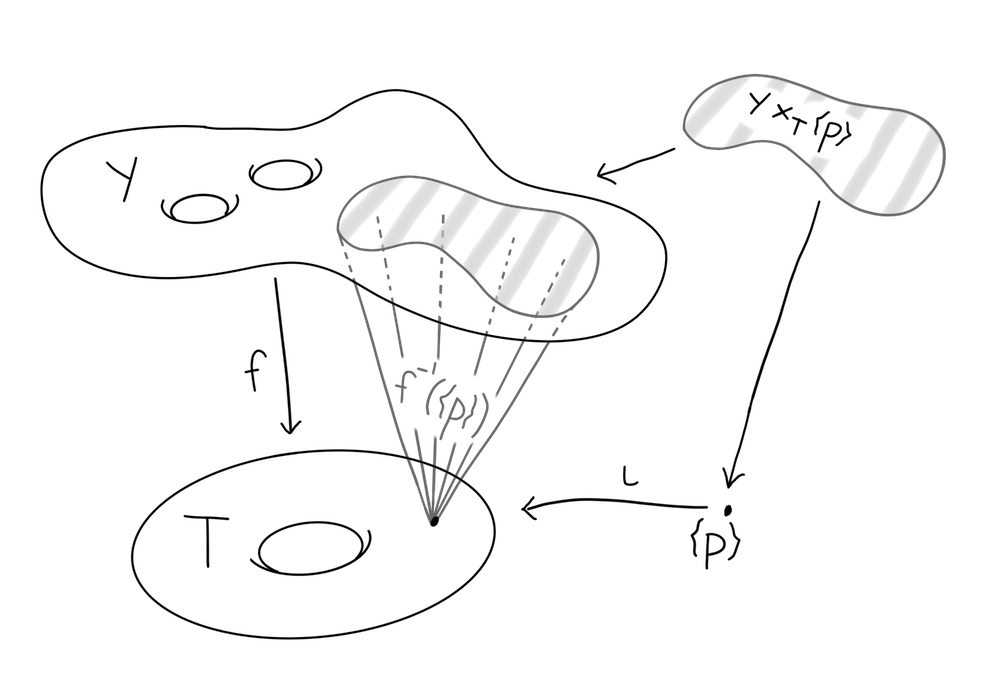
\includegraphics[width=\textwidth]{images/pullback-as-fibre.png}}
                \caption{Pullbacks as fibres}
                \label{fg:pullback-as-fibre}
            \end{minipage}
        \end{figure}

        % \begin{figure}[h]
        %     \centering
        %     \frame{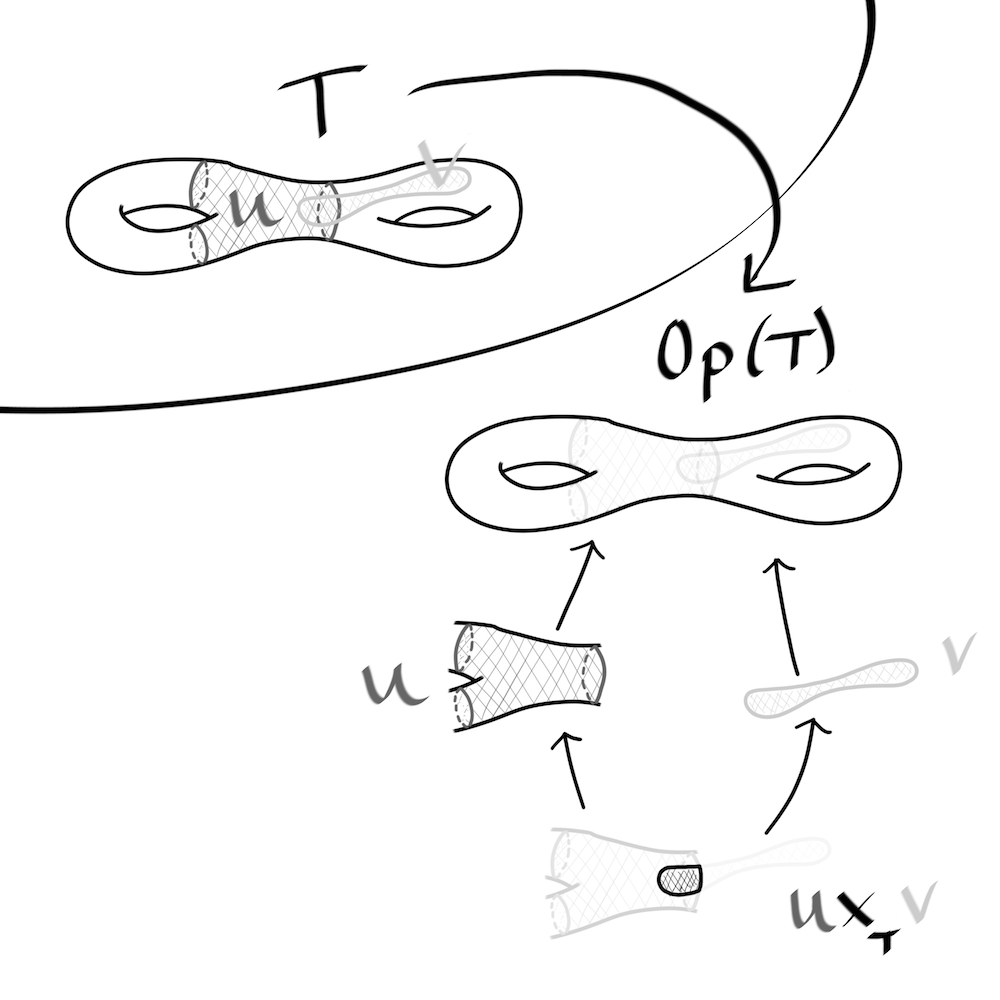
\includegraphics[width=.65\textwidth]{images/opTandpullbacks.png}}
        %     \caption{Pullbacks in $\Op{T}$}
        %     \label{fg:opTandpullbacks}
        % \end{figure}

    % subsubsection exactness_and_pullbacks (end)





    \subsubsection{Grothendieck pseudofunctor} % (fold)
    \label{ssub:a_useful_pseudofunctor}
    
        \begin{definition}[Grothendieck pseudofunctor\footnote{
            This is not standard terminology, but aims to hint at the links to \emph{Grothendieck fibrations} and the \emph{Grothendieck construction}.
            We should probably instead call $M$ a \emph{$\tcat$-indexed category with $\tcat$-indexed coproducts} (see \cite[Definitions~2.1,~3.1]{Ponto:2012wl}).
        } {(Hypothèse~2.1, \S2.1, p.8)}]\label{df:m-t-grothendieck-setup}
            Let $\tcat$ be a category that has finite limits and $M\colon\op{\tcat}\to\Cat$ a pseudofunctor\footnote{
                That is, a `not-quite-functor' $\tcat\to\Cat$ (the category of small categories), in the sense that it doesn't necessarily preserve composition of morphisms and the identity morphism \emph{exactly}, but only up to \emph{coherent isomorphism}.
                Roughly speaking, we require a natural isomorphism $F(g\circ f)\cong F(g)\circ F(f)$ such that we can `evaluate' $F(h)\circ F(g)\circ F(f)$ in an associative way.
                There is a similar condition concerning the identity morphism.
                For more details see \cite[Definition~7.5.1, \S7.5, p.296]{Borceux:1994ws}.
            }.
            Then $M$ is a \emph{Grothendieck pseudofunctor} if it satisfies the following conditions:
            \begin{enumerate}[(i)]
                \item for each $X$ in $\tcat$, the category $M(X)$ has all limits and colimits;
                \item for each $p\colon X'\to X$ in $\tcat$, the functor $M(p)=p^*\colon M(X)\to M(X')$ has a right adjoint $p_*\colon M(X')\to M(X)$ that is conservative;
                \item (\emph{the Beck-Chevalley condition}) for all pullbacks
                    \begin{equation*}
                        \begin{tikzcd}[row sep=.7em]
                             & Y \arrow[dr, "q"] &\\
                            X\times_Z Y \arrow[ur, "p'"] \arrow[dr, swap, "q'"] & & Z\\
                             & X \arrow[ur, swap, "p"] &
                        \end{tikzcd}
                    \end{equation*}
                    in $\tcat$, the natural transformation $p^*q_*\nt q'_*(p')^*$ (called the \emph{change of base}\footnote{
                        See \cref{nt:change-of-base} for information on this terminology.
                    }) is an isomorphism.
                    (\emph{See \cite[\S2,~\P3]{Toen:2005wxa} for how this transformation is constructed}).\qedhere
                    % (See the translation below and \cref{nt:change-of-base})\qedhere
            \end{enumerate}
        \end{definition}

        % \vspace{-2em}

        % \begin{translation}{2}{3}
        %     As a note on condition (iii), the natural transformation in question is constructed in the following way.
        %     We have the natural isomorphisms
        %     \begin{equation*}
        %         (q')^*p^* \cong (pq')^* = (qp')^* \cong (p')^*q^*
        %     \end{equation*}
        %     coming from $M$ being a pseudofunctor.
        %     This gives us, by composing on the right by $q_*$, a natural isomorphism $(q')^*p^*q_*\cong(p')^*q^*q_*$.
        %     By further composing this with the counit $q^*q_*\nt\id$ of the adjuction, we find a natural transformation
        %     \begin{equation*}
        %         (q')^*p^*q_*\nt(p')^*
        %     \end{equation*}
        %     which, by adjuction, gives us
        %     \begin{equation*}
        %         p^*q_*\nt q'_*(p')^*.
        %     \end{equation*}
        %      This is the change of base natural transformation.
        % \end{translation}

        The motivating example for such a pseudofunctor $M$ is when \emph{$\tcat$ is the category of affine schemes and \elide $M(X)$ is the category of quasi-coherent sheaves on $X\in\tcat$} (Remarque~2.2, \S2.1, p.9).

        \begin{figure}[h]
            \centering
            \frame{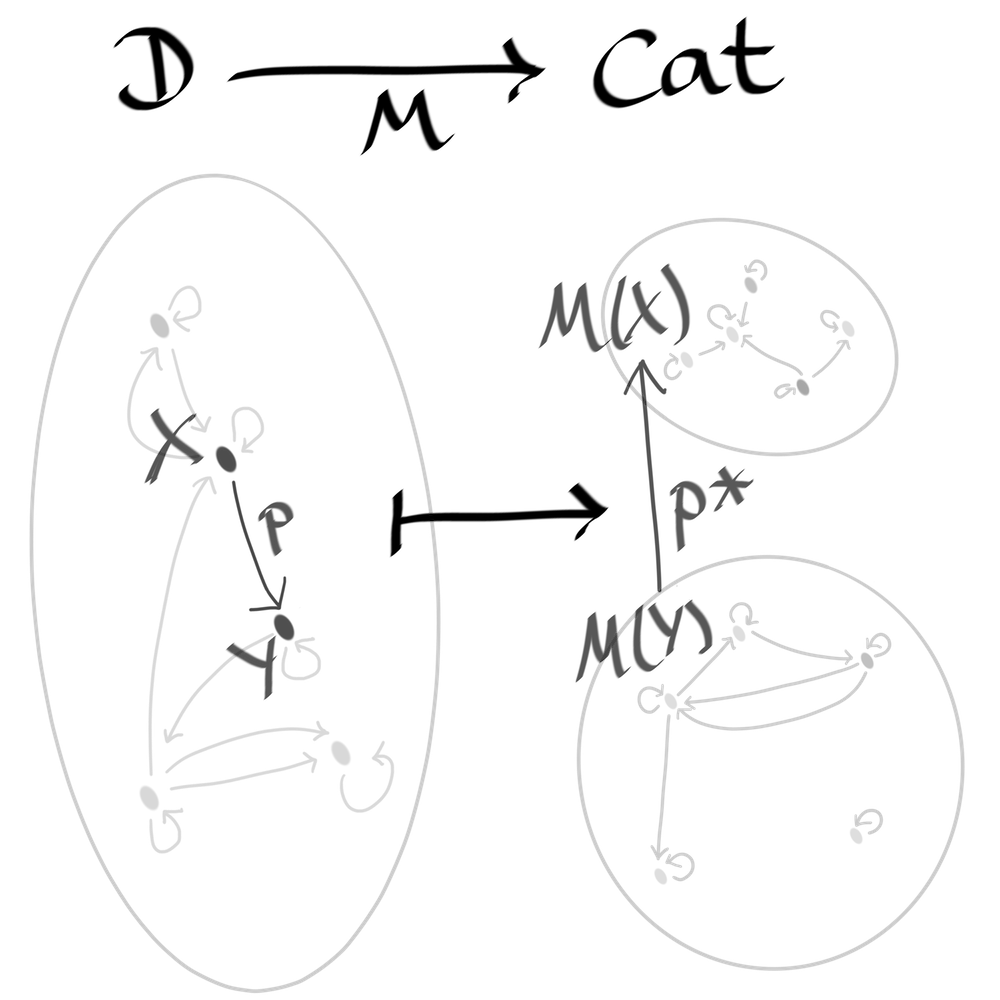
\includegraphics[width=.55\textwidth]{images/grothendieckpseudofunctor.png}}
            \caption{\cref{df:m-t-grothendieck-setup} – note that this is a picture of a contravariant $M\colon\dcat\to\Cat$ rather than a covariant $M\colon\op{\dcat}\to\Cat$.}
            \label{fg:grothendieckpseudofunctor}
        \end{figure}

        \begin{definition}[$M$-faithfully flat {(Définition~2.3, \S2.1, p.9)}]
            Let $\tcat$ and $M$ be as in \cref{df:m-t-grothendieck-setup}, and let $\famofmor$ be a family of morphisms in $\tcat$.
            Then $\famofmor$ is
            \begin{enumerate}[(i)]
                \item \emph{$M$-covering} if there exists a finite (non-empty) subset $J\subset I$ such that the family of functors
                \begin{equation*}
                    \{p_j^*\colon M(X)\to M(X_j)\}_{j\in J}
                \end{equation*}
                is conservative;
                \item \emph{$M$-flat} if all the functors $p_i^*\colon M(X)\to M(X_i)$ are left exact\footnote{
                    Note that, by \cref{df:m-t-grothendieck-setup}, a morphism $p\colon X'\to X$ is $M$-flat if and only if the functor $p^*$ is \emph{exact}.
                    This is because left adjoint functors are right exact (\cref{co:adjoint-exactness}) and we have assumed that $p^*$ \emph{has} a right adjoint (\cref{df:m-t-grothendieck-setup}).
                };
                \item \emph{$M$-faithfully flat} if it is both $M$-covering and $M$-flat.\qedhere
            \end{enumerate}
        \end{definition}

        The reason for the name `$M$-faithfully flat' comes from the fact that \emph{if $p$ is $M$-faithfully flat then $p^*$ is faithful}\footnote{
            We provide here a quick proof.
            Since $M(X)$ is bicomplete we have a \emph{zero object} and the notion of an \emph{equaliser} (dual to \cref{df:coequaliser}).
            By definition, two morphisms $f,g$ in $M(X)$ are equal if and only if their equaliser is zero.
            Now $p^*$ is exact, so it commutes with limits.
            Thus $\eq(p^*(f)\rightrightarrows p^*(g))\cong\eq(p^*(f\rightrightarrows g))$.
            Further, since $p^*$ is exact, $p^*(0)=0$.
            Also, since $p^*$ is conservative, it reflects limits, so $[p^*(c)=0\implies c=0]$.
            Thus $p^*(c)=0$ if and only if $c=0$.
            Putting these facts together we see that $f=g$ if and only if $p^*(f)=p^*(g)$.
            That is, $p^*$ is faithful.
        } (\S2.1 \P5).

    % subsubsection a_useful_pseudofunctor (end)





    \subsubsection{Grothendieck topologies} % (fold)
    \label{ssub:grothendieck_topologies}
    
        Classically, we use a topology on a commutative $k$-algebra (or commutative ring) to define the notion of a \emph{sheaf}.
        One of the pivotal moments for algebraic geometry (and mathematics as a whole) was Groethendieck's generalisation of this idea in 1958, rephrased in terms of category theory (which was itself only around 13 years old).
        The foundational definition was that of a \emph{site}, which is a category endowed with a \emph{Grothendieck topology}\footnote{
            We sometimes refer to this simply as a \emph{topology}, but only when it is obvious what we mean.
        } -- a structure that mirrored that of open sets of a topological space\footnote{
            Though there is some confusion with this nomenclature; \cite{Johnstone:2002wb} suggests the name \emph{Grothendieck coverage}, but we stick with `topology' for simplicity.
            See \cite{Skoda:2011wq}.
        }.
        There is also a \emph{Grothedieck pretopology}, which is slightly less strict, but can be used to construct a topology.
        We formalise all of this below.

        \begin{definition}[Grothendieck pretopology {(\cite{Schreiber:8YBVOVEM})}]\label{df:grothendieck-pretopology}
            Let $\ccat$ be a category with pullbacks.
            A \emph{Grothendieck pretopology on $\ccat$} is an assignment, to each object $X\in\ccat$, of a collection $C(X)$ of families of morphisms to $X$, called \emph{covering families}, satisfying the following conditions for all $X\in\ccat$:
            \begin{enumerate}[(i)]
                \item (\emph{isomorphisms cover}) for every isomorphism $Y\congto X$ in $\ccat$, the singleton family $\{Y\congto X\}$ is in $C(X)$;
                \item (\emph{stability}) the collection $C(X)$ is stable under pullback (or change of base): if $\{X_i\to X\}\in C(X)$ and $f\colon Y\to X$ is some arbitrary morphism in $\ccat$, then $\{f^* X_i\to Y\}_{i\in I}\in C(Y)$, where $f^*X_i=(Y\times_X X_i)$;
                \item (\emph{transitivity}) if $\{X_i\to X\}_{i\in I}\in C(X)$ and there is a covering family $\{X_{i,j}\to X_i\}_{j\in J_i}\in C(X_i)$ for each $i\in I$, then the family of composites $\{X_{i,j}\to X_i\to X\}_{i\in I,j\in J_i}$ is also in $C(X)$.\qedhere
            \end{enumerate}
        \end{definition}

        \begin{figure}[h]
            \centering
            \frame{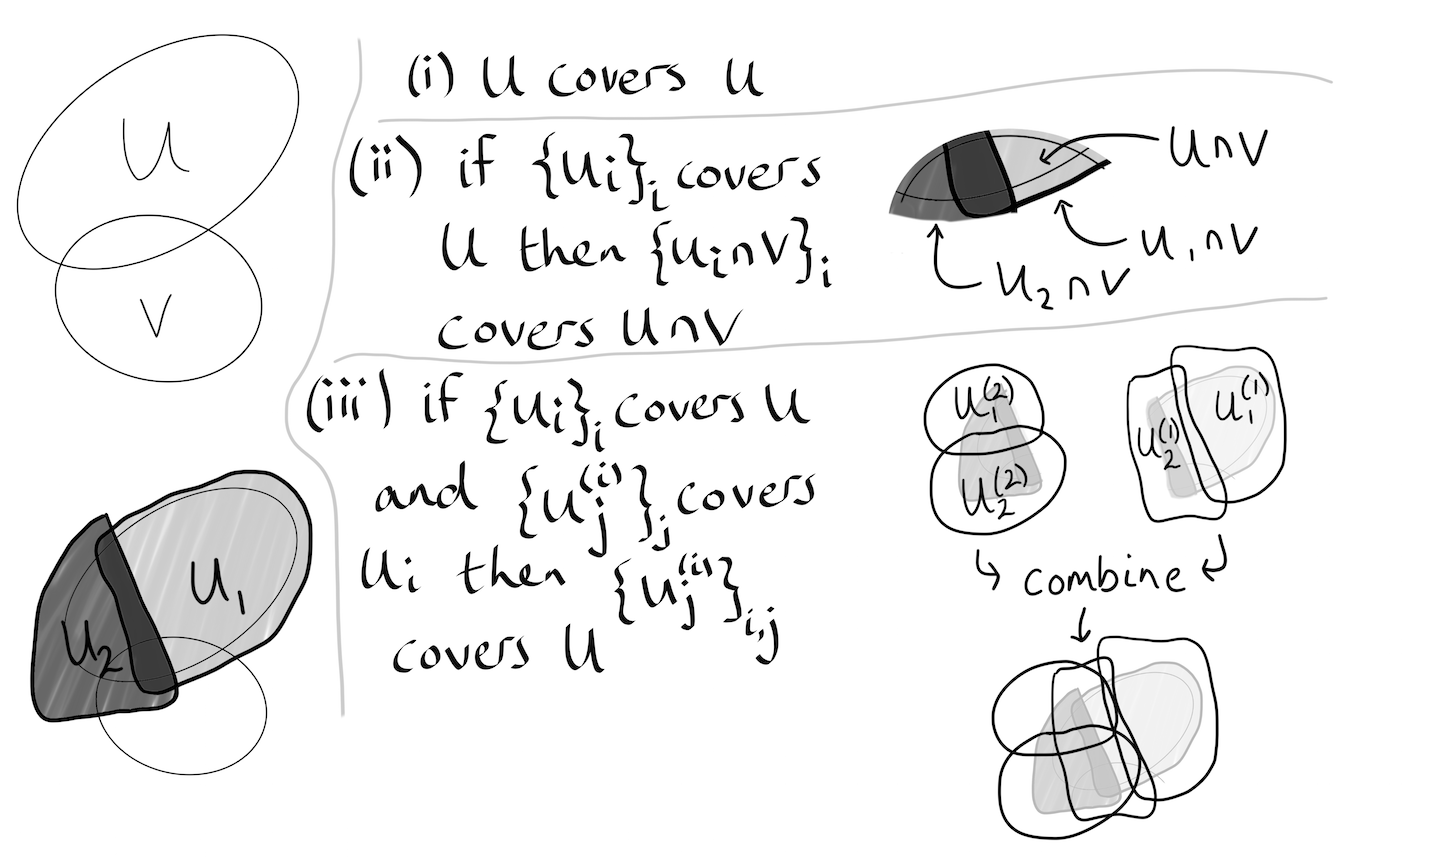
\includegraphics[width=.9\textwidth]{images/grothendieckpretopologyNEW.png}}
            \caption{\cref{df:grothendieck-pretopology} with $\ccat=\Op{T}$}
            \label{fg:grothendieckpretopology}
        \end{figure}

        The previously-introduced notion of `$M$-faithfully flat' now comes into use: such families can be used to construct a pretopology.

        \begin{lemma}[(Proposition~2.4, \S2.1, p.9)]\label{le:m-t-grothendieck-pretopology}
            Let $\tcat$ and $M$ be as in \cref{df:m-t-grothendieck-setup}.
            Then the $M$-faithfully flat families define\footnote{
                To each $X\in\tcat$ we assign the collection $C(X)$ of $M$-faithfully flat families $\{X_i\to X\}$.
            } a Grothendieck pretopology on $\tcat$.
        \end{lemma}

        \begin{proof}
            \mbox{}
            \begin{enumerate}[(i)]
                \item (\emph{Isomorphisms cover})
                    Let $p\colon Y\congto X$ be some isomorphism in $\dcat$.
                    We want $p^*\colon M(X)\to M(Y)$ to be conservative and left exact.
                    If we have $p^*\cong(p^{-1})_*$ then left exactness follows from being a right adjoint, and being conservative follows from \cref{df:m-t-grothendieck-setup}.

                    Since $M$ is a pseudofunctor, we have natural isomorphisms
                    \begin{align*}
                        (p^{-1})_*p_*\cong(pp^{-1})_*\cong&\id_{M(X)}\\
                        &\id_{M(Y)}\cong(p^{-1}p)_*\cong p_*(p^{-1})_*
                    \end{align*}
                    Thus $(p^{-1})_*\dashv p_*$ and so $(p^{-1})_*\cong p^*$ as required.
                \item (\emph{Stability})
                    Let $\{p_i\colon X_i\to X\}$ be $M$-faithfully flat and $f\colon Y\to X$.
                    Define $Y_i=Y\times_X X_i$ with morphisms
                    \begin{equation*}
                        \begin{tikzcd}[column sep=1em, row sep=.5em]
                            & Y \arrow[dr, "f"] &\\
                            Y_i \arrow[ur, "q_i"] \arrow[dr, swap, "f_i"] & & X\\
                            & X_i \arrow[ur, swap, "p_i"] &
                        \end{tikzcd}
                    \end{equation*}
                    We want to show that $\{q_i\colon Y_i\to Y\}$ is $M$-faithfully flat.

                    Firstly, to be $M$-covering we want
                    \begin{equation*}
                        \left(\prod_{j\in J} q_j^*\right)\colon M(Y)\to \prod_{j\in J} M(Y_j)
                    \end{equation*}
                    to be conservative for some finite $J\subset I$.
                    We claim that the same finite $J\subset I$ that makes $\{p_i\}$ $M$-covering works.
                    By \cref{df:m-t-grothendieck-setup}, $(f_i)_*$ is conservative, and so the above morphism is conservative if and only if
                    \begin{equation*}
                        \left(\prod_{j\in J} (f_j)_*q_j^*\right)\colon M(Y)\to \prod_{j\in J} M(X_j)
                    \end{equation*}
                    is conservative.
                    Now, $p_i^*f_*\cong(f_i)_*q_i^*$, so the above morphism is conservative if and only if
                    \begin{equation*}
                        \left(\prod_{j\in J} p_i^* f_*\right)\colon M(Y)\to \prod_{j\in J} M(X_j)
                    \end{equation*}
                    is conservative.
                    But both $f_*$ and $\{p_j^*\}_{j\in J}$ are conservative, so we are done.

                    Secondly, to be $M$-flat we want $q_i^*$ to be left exact for all $i\in I$.
                    This follows straight from $p_i^*f_*\cong(f_i)_*q_i^*$, since both $f_*$ and $(f_i)_*$ are right adjoints, thus left exact, and $p_i^*$ is left exact by hypothesis.
                \item (\emph{Transitivity})
                    Let $\{p_i\colon X_i\to X\}_{i\in I}$ be $M$-faithfully flat.
                    Suppose we also have $M$-faithfully flat $\{q^{(i)}_j\colon Y^{(i)}_j\to X_i\}_{j\in J}$ for all $i\in I$.
                    The fact that
                    \begin{equation*}
                        \{p_iq^{(i)}_j\colon Y^{(i)}_j\to X\}_{(i,j)\in I\times J}
                    \end{equation*}
                    is $M$-covering follows from the fact that the product of two finite sets is finite; that it is $M$-flat follows from the natural isomorphisms $(p_i q^{(i)}_j)^*\cong (q^{(i)}_j)^* p_i^*$ and the fact that the composition of two left-exact functors is again left exact.\qedhere
            \end{enumerate}
        \end{proof}

        \begin{definition}[Sieves on an object]
            Let $X\in\ccat$ be an object in some category.
            A \emph{sieve on $X$} is a subset\footnote{
                Again, we are assuming local smallness here for simplicity.
            } $S\subset \ccat/X$ of the objects of the slice category that is \emph{saturated} (i.e. closed under precomposition).
            That is, if $(Y\to X)\in S$ and $Y'\to Y$ is some arbitrary morphism in $\ccat$, then the composition $Y'\to Y\to X$ is also in $S$.
        \end{definition}

        If we have any collection $C$ of morphisms to some fixed object $X\in\ccat$ then we can \emph{saturate} the collection to obtain a sieve on $X$ -- we can extend the collection to include all precompositions by arbitrary morphisms to any object that is the source of a morphism in $C$.

        \begin{definition}[Pullback sieve]\label{df:pullback-sieve}
            Let $\ccat$ be some category, $S$ a sieve on $X\in\ccat$, and $f\colon Y\to X$ some morphism in $\ccat$.
            Then the \emph{pullback of $S$ along $f$}, written $f^* S$, is the sieve on $Y$ defined by\footnote{
                Roughly speaking, take all morphisms to $X$ that factor through $Y$ along $f$ and `divide them by $f$'.
            }
            \begin{equation*}
                f^* S = \{g\in\Hom(Y', Y) \mid Y\in\ccat,fg\in S\}.\qedhere
            \end{equation*}
        \end{definition}

        As to why this construction is called a pullback, we recall \cref{df:pullbacks} and claim that $f^* S$ is the image\footnote{
            Which we can avoid defining category-theoretically here since we have a natural underlying set structure.
        } of the projection
        \begin{equation*}
            S\times_{\Hom(\blank, X)}\Hom(\blank, Y) \to \Hom(\blank, Y)
            % \begin{array}{c}
                % S\times_{\Hom(\blank, X)}\Hom(\blank, Y)\\
            %     \Big\downarrow\\
            %     \Hom(\blank, Y)
            % \end{array}
        \end{equation*}
        where we take the pullback in $\Set$, and our morphisms are the inclusion $S\hookrightarrow\Hom(\blank, X)$ and post composition $(f\circ\blank)\colon\Hom(\blank, Y)\to\Hom(\blank, X)$.
        It follows from \cref{df:pullbacks} that, in $\Set$, the pullback is given by
        \begin{equation*}
            X\prescript{\varphi}{}{\times}^\psi_Z Y = \{(x,y)\in X\times Y \mid \varphi(x)=\psi(y)\}.
        \end{equation*}
        So here,
        \begin{equation*}
            S\times_{\Hom(\blank, X)}\Hom(\blank, Y) = \{(g,h)\in S\times\Hom(\blank, Y) \mid g=f\circ h\}
        \end{equation*}
        and projecting this to $\Hom(\blank, Y)$ gives the set of all morphisms $h$ such that $f\circ h=g$ for some $g\in S$.
        This is exactly what \cref{df:pullback-sieve} says.

        \begin{definition}[Grothendieck topology\footnote{
            As in \cite{Schreiber:2009wl}.
        }]\label{df:grothendieck-topology}
            Let $\ccat$ be some category.
            A \emph{Grothendieck topology on $\ccat$} is an assignment, to each object $X\in\ccat$, of a collection $J(X)$ of sieves on $X$, called \emph{covering sieves}, such that the following conditions are satisfied for all $X\in\ccat$:
            \begin{enumerate}[(i)]
                \item (\emph{base change}) if $S\in J(X)$ and $f\colon Y\to X$ is some arbitrary morphism in $\ccat$, then the pullback sieve satisfies $f^* S\in J(Y)$;
                \item (\emph{maximal sieve}) $\Hom(\blank,X)\in J(X)$;
                \item (\emph{intersections})\footnote{
                    This condition is actually redundant; see the comments after \cite[Definition~1,~\S III.2]{MacLane:1992uz}.
                } $S,T\in J(X)$ if and only if $S\cap T\in J(C)$;
                \item (\emph{transitivity}) if $S\in J(X)$ is such that $T_S\in J(X)$, where
                    \begin{equation*}
                        T_S=\bigcup_{Y\in\ccat}\{f\colon Y\to X \mid f^* S\text{ is covering on }Y\},
                    \end{equation*}
                    then $S\in J(X)$.\qedhere
            \end{enumerate}
        \end{definition}

        \begin{definition}[Site]\label{df:site}
            Let $\ccat$ be a category and $J$ a Grothendieck topology on $\ccat$.
            Then the pair $(\ccat,J)$ is called a \emph{site}.
        \end{definition}

        Recall: a pretopology on a category $\ccat$ consists of, for each $X\in\ccat$, a collection $C(X)$ of covering families $\{X_j\to X\}$.
        We can use these to pick certain sieves on $X$ that we wish to be in $J(X)$, and then see that this choice satisfies the conditions of \cref{df:grothendieck-topology}.
        The actual method is quite simple: given some sieve $S=\{S_i\to X\}$ on $X$, we say that $S\in J(X)$ if and only if it contains some covering family $\{X_j\to X\}\in C(X)$.
        More details on this construction can be found in \cite[\S III.2]{MacLane:1992uz}.

        % \begin{note}[Summary]\label{nt:make-topologies-with-m}
        %     \emph{The overall result of this section is as follows:} we can construct a Grothendieck topology on some category $\tcat$ (that has finite limits) by constructing some Grothendieck pseudofunctor $M$ and considering $M$-faithfully flat families.
        % \end{note}

        \begin{note}\label{nt:no-theorem-2.5}
            There is an important result (\cite[Théorème~2.5, \S2.1, p.11]{Toen:2005wxa}) that we don't cover here because it deals with the notion of \emph{stacks}.
            % Roughly speaking, a stack is like a sheaf, but whereas a sheaf is obtained by gluing together sets, a stack is obtained by gluing together categories.
            % Since categories have a much richer structure than sets (most notably, they have morphisms) the gluing is slightly more complicated, and needs the idea of \emph{descent data}, which is the abstract analogue of gluing.
            We do not have the space in this paper to cover the background needed to talk about stacks; we refer the interested reader back to \cite{Toen:2005wxa}.
            From now on we will skip over stack-theoretic theorems without mentioning them.
        \end{note}

    % subsubsection grothendieck_topologies (end)

% subsection constructing_grothendieck_topologies (end)


% !TEX root = ../../../under-spec-z.tex

\subsection{The faithfully flat topology} % (fold)
\label{sub:the_faithfully_flat_topology}

    \emph{Throughout this section $\smc$ is a cosmos\footnote{
            In keeping with Hypothèse 2.6, \S2.2, p.14; recalling \cref{df:cosmos}.
        } and we use $\dcat$ to refer to an arbitrary category.}
    % We start this section by introducing a fundamental definition -- that of an \emph{affine scheme over a cosmos}.
    \emph{The structure of this section is largely based on \cite[\S1.2,~1.3]{Marty:2009tj} (where all proofs can be found) and \cite[\S1.1]{Toen:2008wy}.}

    \begin{definition}[Affine schemes over $\ccat$ {(Définition 2.7, \S2.2, p.14)}]\label{df:old-affine-schemes}
        The category of \emph{affine schemes over $\ccat$} is the opposite category
        \begin{equation*}
            \aff{\ccat}=\op{\comm{\ccat}}.
        \end{equation*}
        For an object $A\in\comm{\ccat}$ we write $\spec A$ to denote the corresponding object in $\aff{\ccat}$.
    \end{definition}

    % \subsubsection{Introduction to changes of base} % (fold)
    % \label{ssub:introduction_to_changes_of_base}

    %     \begin{definition}[Slice category]\label{df:slice-category}
    %         Let $\dcat$ be some category and $X\in\dcat$ some object.
    %         We define the \emph{slice category $\dcat/X$} (sometimes called the \emph{over category} and sometimes written \emph{$\dcat\downarrow X$}) as having
    %         \begin{itemize}
    %             \item \emph{objects:} morphisms $Y\to X$ in $\dcat$ for some $Y\in\dcat$;
    %             \item \emph{morphisms:} morphisms $Y\to Y'$ in $\dcat$ such that
    %                 \begin{equation*}
    %                     \begin{tikzcd}[column sep=1em]
    %                         Y \arrow[dr] \arrow[rr] & & Y' \arrow[dl]\\
    %                          & X & \\
    %                     \end{tikzcd}
    %                 \end{equation*}
    %                 commutes.\qedhere
    %         \end{itemize}
    %     \end{definition}

    %     Dually, we have the the \emph{coslice} (or \emph{under}) category $X/\dcat$: its objects are morphisms $X\to Y$, and its morphisms are morphisms $Y\to Y'$ making the induced triangle commute.
    %     Since the only difference between slice and coslice categories is the direction of the arrows, it makes sense to think that there might be some relation between the two in terms of opposite categories.
    %     The following lemma makes this relation explicit, and although we have no use for it at the moment, it proves useful later on.

    %     \begin{lemma}\label{le:op-coslice-slice}
    %         Let $\dcat$ be some category and $X\in\dcat$.
    %         Then $\op{(X/\dcat)} \cong \op{\dcat}/X$.
    %     \end{lemma}

    %     \begin{proof}
    %         TJH todo
    %     \end{proof}

    %     TJH mention what \cref{le:op-coslice-slice} means for functors!

    %     Once again, we now introduce a purely category-theoretic notion which we will later apply to our scenario.

    %     \begin{definition}[Change of base]
    %         Let $\dcat$ be a category with pullbacks, and $f\colon X\to Y$ a morphism in $\dcat$.
    %         Then the \emph{change of base functor $f^*\colon \dcat/Y\to\dcat/X$} is the induced functor given, on objects, by the pullback along $f$:
    %         \begin{equation*}
    %             \left(
    %                 \begin{tikzcd}
    %                     X' \arrow[d, "p"]\\
    %                     Y
    %                 \end{tikzcd}
    %             \right)
    %             \mapsto
    %             \left(
    %                 \begin{tikzcd}
    %                     X\prescript{f}{}{\times}^p_Y X' \arrow[d, "\pi_X"]\\
    %                     X
    %                 \end{tikzcd}
    %             \right)
    %         \end{equation*}
    %         and we write $p^*=f^*(p)=\pi_X$.
    %     \end{definition}

    % % subsubsection introduction_to_changes_of_base (end)


    \subsubsection{Commutative algebras} % (fold)
    \label{ssub:commutative_algebras}

        \begin{definition}[Commutative $A$-algebras]
            Let $A\in\comm{\ccat}$.
            The objects of $A/\comm{\ccat}$ are called \emph{commutative $A$-algebras}, and we write $\algc{A}$ to mean the category of such objects.
        \end{definition}

        This slightly opaque definition is best explained after showing how we can endow $\modc{A}$ with a symmetric monoidal structure.

        \begin{definition}[Coequaliser]\label{df:coequaliser}
            The \emph{coequaliser $\coeq(X\rightrightarrows Y)$} of two morphisms $f,g\colon X\to Y$ in $\dcat$ is defined by the universal property of being a pair $(Q,q)$, where $Q\in\dcat$ and $q\colon Y\to Q$, such that $q\circ f=q\circ g$, and for any other such pair $(R,r)$ there exists a unique morphism $\varphi\colon Q\to R$ such that the following diagram commutes:
            \begin{equation*}
                \begin{tikzcd}
                    X \arrow[r, shift left=.75ex, "f"] \arrow[r, shift right=.75ex, swap, "g"] & Y \arrow[r, "q"] \arrow[dr, "r"] & Q \arrow[d, dotted, "\varphi"]\\
                     & & R
                \end{tikzcd}
            \end{equation*}
        \end{definition}
        \vspace{-3em}
        \begin{definition}[Symmetric monoidal structure on $\modc{A}$]\label{df:smc-on-a-mod}
            Let $A\in\comm{\ccat}$.
            Define the bifunctor $(\blank\otimes_A\blank)\colon\modc{A}\times\modc{A}\to\modc{A}$ by the object of the coequaliser
            \begin{equation*}
                X\otimes_A Y = \coeq(X\otimes A\otimes Y\rightrightarrows X\otimes Y),
            \end{equation*}
            where the morphisms are the natural ones, namely
            \begin{align*}
                X\otimes (A\otimes Y) &\xrightarrow{\id_X\otimes\sigma_Y} X\otimes Y\\
                (X\otimes A)\otimes Y &\xrightarrow{(\sigma_X\circ\gamma_{XA})\otimes\id_Y} X\otimes Y.
            \end{align*}
            Then $(\modc{A},\otimes_A,A)$ is a symmetric monoidal category\footnote{
                \cite[Proposition~1.2.15,~\S1.2,~p.14]{Marty:2009tj}
            }.
        \end{definition}

        \begin{lemma}[Equivalent definitions of $\algc{A}$]\label{le:two-definitions-of-alg}
            Let $A\in\comm{\ccat}$.
            Then we have the equivalence of categories
            \begin{equation*}
                \comm{\modc{A}} \equiv \algc{A} = A/\comm{\ccat}
            \end{equation*}
            (using the symmetric monoidal structure from \cref{df:smc-on-a-mod}).
        \end{lemma}

        \begin{proof}
            \cite[Proposition~1.2.15,~\S1.2,~p.14]{Marty:2009tj}.
        \end{proof}

        Because of this equivalence we sometimes write objects of $\algc{A}$ as $X$ for some $X\in\comm{\modc{A}}$, and sometimes as $(A\to X)$ for some $X\in\comm{\ccat}$.
        Object-wise, we can think of the structures we have defined as follows:
        \begin{equation*}
            \comm{\modc{A}}\equiv\algc{A}\subset\modc{A}\subset\comm{\ccat}\subset\ccat.
        \end{equation*}

        % \begin{lemma}\label{le:commcatt-and-modca-bicomplete}
        %     Both $\comm{\ccat}$ and $\modc{A}$ are bicomplete, for all $A\in\comm{\ccat}$.
        % \end{lemma}

        % \begin{proof}
        %     \cite[Proposition~1.2.14,~\S1.2,~p.11]{Marty:2009tj}
        % \end{proof}

        % \begin{lemma}\label{le:modc-a-is-closed}
        %     Let $A\in\comm{\ccat}$.
        %     Then $(\modc{A},\otimes_A,A)$ is a closed symmetric monoidal category.
        % \end{lemma}

        % \begin{proof}
        %     \cite[Proposition~1.2.17,~\S1.2,~p.17]{Marty:2009tj}
        % \end{proof}

        \begin{corollary}\label{le:modc-a-cosmos-algc-a-bicomplete}
            Let $A\in\comm{\ccat}$.
            Then
            \begin{enumerate}[(i)]
                \item $\comm{\ccat}$ and $\algc{A}$ are bicomplete;
                \item $(\modc{A},\otimes_A,A)$ is a cosmos.\qedhere
            \end{enumerate}
        \end{corollary}

        \begin{proof}
            \cref{le:two-definitions-of-alg} and \cite[Propositions~1.2.14,~1.2.17~\S1.2]{Marty:2009tj}.
        \end{proof}

        \begin{lemma}\label{le:otimes-is-sqcup}
            Let $A\in\comm{\ccat}$ and $X,Y\in\comm{\modc{A}}$.
            Then
            \begin{equation*}
                X\otimes_A Y\cong X\sqcup_A Y
            \end{equation*}
            where the coproduct is taken in $\comm{\ccat}$.
        \end{lemma}

        \begin{proof}
            \cite[Proposition~1.2.6,~\S1.2,~p.16]{Marty:2009tj}
        \end{proof}
    
    % subsubsection commutative_algebras (end)


    \subsubsection{Change of base for modules over a monoid} % (fold)
    \label{ssub:change_of_base_for_modules_over_a_monoid}

        Assume we have some morphism $f\colon\spec B\to\spec A$ in $\aff{\ccat}$.
        We claim that this induces a forgetful functor $\modc{B}\to\modc{A}$.
        That is, on the level of objects, $\modc{B}\subset\modc{A}$.

        Take some object $X\in\modc{B}$.
        This comes with a $B$-action $\sigma_B\colon B\otimes X\to X$.
        We can compose $f$ and $\sigma_B$ to obtain
        \begin{equation*}
            \sigma_A\colon A\otimes X \xrightarrow{f\otimes\id_X} B\otimes X \xrightarrow{\sigma_B} X.
        \end{equation*}
        We claim that this is an $A$-action on $X$.
        This just means showing that both of the diagrams in \cref{df:module-over-monoid} commute.
        Here we show just one since the other is equally straightforward.
        Note that
        \begin{equation*}
            \begin{tikzcd}[row sep=2em,column sep=1em]
                1\otimes X \arrow[rr, "\eta_A\otimes\id_X"] \arrow[dr, swap, "\lambda_X"] & & A\otimes X \arrow[dl, "\sigma_A"]\\
                 & X &
            \end{tikzcd}
            =
            \begin{tikzcd}[row sep=2em,column sep=1em]
                1\otimes X \arrow[rr, "(f\circ\eta_A)\otimes\id_X"] \arrow[dr, swap, "\lambda_X"] & & B\otimes X \arrow[dl, "\sigma_B"]\\
                 & X &
            \end{tikzcd}
        \end{equation*}
        But $f$ is a morphism in $\comm{\ccat}$, so \mbox{$f\circ\eta_A=\eta_B$} (recall \cref{df:comm-c}), and hence the second diagram commutes.
        Thus so too does the first diagram.
        We also have an induced forgetful functor $\algc{B}\to\algc{A}$, since if $(B\to X)\in\algc{B}$ then, composing with $f$, we get $(A\to B\to X)\in\algc{A}$.
        
        We mention the forgetful functor $\modc{B}\to\modc{A}$ because it has a left-adjoint, namely
        \begin{equation*}
            (\blank\otimes_A B)\colon\modc{A}\to\modc{B}
        \end{equation*}
        (which is well defined: $f$ lets us consider $B$, which is a $B$-module, as an $A$-module).
        This tells us that $(\blank\otimes_A B)$ is right exact.


        % The functor $(\blank\otimes_A B)\colon\modc{A}\to\modc{B}$ also arises naturally in another way though: it is the change of base functor in $\aff{\ccat}$.
        % To see this, start again with some morphism $f\colon\spec B\to\spec A$ in $\aff{\ccat}$.
        % Then the change of base functor
        % \begin{align*}
        %     f^*\colon \aff{\ccat}/\spec A &\longrightarrow \aff{\ccat}/\spec B\\[1em]
        %     \left(
        %         \begin{array}{c}
        %             X\\
        %             \downarrow\\
        %             \spec A
        %         \end{array}
        %     \right) &\mapsto
        %     \left(
        %         \begin{array}{c}
        %             \spec B\times_{\spec A} X\\
        %             \downarrow\\
        %             \spec B
        %         \end{array}
        %     \right)
        % \end{align*}
        % is tautologically equivalent to the functor
        % \begin{align*}
        %     f^*\colon \op{\comm{\ccat}}/A &\longrightarrow \op{\comm{\ccat}}/B\\[1em]
        %     \left(
        %         \begin{array}{c}
        %             X\\
        %             \downarrow\\
        %             A
        %         \end{array}
        %     \right) &\mapsto
        %     \left(
        %         \begin{array}{c}
        %             B\times_A X\\
        %             \downarrow\\
        %             B
        %         \end{array}
        %     \right)\\
        % \end{align*}
        % which is equivalent to the functor
        % \begin{align*}
        %     g^*\colon A/\comm{\ccat} &\longrightarrow B/\comm{\ccat}\\[1em]
        %     \left(
        %         \begin{array}{c}
        %             A\\
        %             \downarrow\\
        %             X
        %         \end{array}
        %     \right) &\mapsto
        %     \left(
        %         \begin{array}{c}
        %             B\\
        %             \downarrow\\
        %             B\sqcup_A X
        %         \end{array}
        %     \right)
        % \end{align*}
        % by \cref{le:op-coslice-slice}.

        % Now $B\sqcup_A X\cong X\sqcup_A B$ (\textbf{TJH PROVE THIS or at least say why}), and both $A$ and $X$ are $B$-algebras (since we have, by definition, morphisms to both from $B$).
        % So \cref{le:otimes-is-sqcup} tells us that the change of base functor
        % \begin{equation*}
        %     f^*\colon\aff{\ccat}/\spec A\to\aff{\ccat}/\spec B
        % \end{equation*}
        % is simply
        % \begin{equation*}
        %     (\blank\otimes_A B)\colon\modc{A}\to\modc{B}
        % \end{equation*}
        % (after using the forgetful functor $\algc{A}=A/\comm{\ccat}\to\comm{\ccat}$).

        % \emph{TJH extending from $\algc{A}$ to $\modc{A}$?}
        
        % \textbf{TJH i am not really very certain about all of this -- check!}
    
    % subsubsection change_of_base_for_modules_over_a_monoid (end)


    \subsubsection{fpqc topology} % (fold)
    \label{ssub:fpqc_topology}
    
        Now we apply the results from \cref{ssub:commutative_algebras,ssub:change_of_base_for_modules_over_a_monoid}.
        Let $\tcat=\aff{\ccat}$ and, using $\op{(\aff{\ccat})}=\comm{\ccat}$, define the pseudofunctor
        \begin{align}\label{eq:m-and-d-for-fpqc}
            M\colon\op{(\aff{\ccat})}&\to\Cat\\[.35em]
            A&\mapsto\modc{A}\nonumber\\
            (A\to B)&\mapsto(\blank\otimes_A B\colon\modc{A}\to\modc{B}).\nonumber
        \end{align}
        We claim that $\tcat$ and $M$ satisfy the conditions of \cref{df:m-t-grothendieck-setup}, and so generate a Grothendieck topology on $\aff{\ccat}$.
        There are four conditions that we need to check\footnote{
            Really, we also need to check that $M$ actually \emph{is} a pseudofunctor, but since we only gave a rough definition of pseudofunctors we simply claim that this is, in fact, true.
        }:
        \begin{enumerate}[(i)]
            \item \emph{$\aff{\ccat}$ has finite limits}: \cref{le:modc-a-cosmos-algc-a-bicomplete} (recall that $\aff{\ccat}=\op{\comm{\ccat}}$);
            \item \emph{$\modc{A}$ is bicomplete}: \cref{le:modc-a-cosmos-algc-a-bicomplete};
            \item \emph{$(\blank\otimes_A B)$ has a conservative right adjoint}: the right adjoint is the forgetful functor $\modc{B}\to\modc{A}$, and this is conservative since it gives us $\modc{B}$ as a full subcategory of $\modc{A}$;
            \item \emph{the Beck-Chevalley condition}\footnote{
                This is proved (much more generally) in \cite[Example~2.35]{Shulman:2013tx}.
            }: say we have the following pullback diagram
            \begin{equation*}
                \begin{tikzcd}[row sep=.7em]
                     & \spec B \arrow[dr, "q"] &\\
                    \spec X \arrow[ur, "p'"] \arrow[dr, swap, "q'"] & & \spec C\\
                     & \spec A \arrow[ur, swap, "p"] &
                \end{tikzcd}
            \end{equation*}
            in $\aff{\ccat}$ (i.e. $\spec X=\spec B\times_{\spec C}\spec A$ is the pullback).
            Then $X=B\sqcup_C A$ is the pushout in $\comm{\ccat}$, and $A,B\in\comm{\modc{C}}\equiv\algc{C}$.
            \Cref{le:otimes-is-sqcup} then tells us that $X\cong B\otimes_C A$.
            Thus\footnote{
                The second isomorphism comes from associativity; the third comes from the fact that $M\otimes_B B\cong M$.
                Both these facts mirror the usual case of tensor products over a commutative ring, and can be proved by using \cref{le:otimes-is-sqcup}: $X\otimes_A Y\cong X\sqcup_A Y$.
            }, for $M\in\modc{B}$,
            \begin{equation*}
                M\otimes_B X \cong M\otimes_B(B\otimes_C A) \cong (M\otimes_B B)\otimes_C A \cong M\otimes_C A,
            \end{equation*}
            and so $p^*q_*=(\blank\otimes_C A)\cong(\blank\otimes_B X)=(q')_*(p')^*$.
        \end{enumerate}

        \begin{figure}[h]
            \centering
            \frame{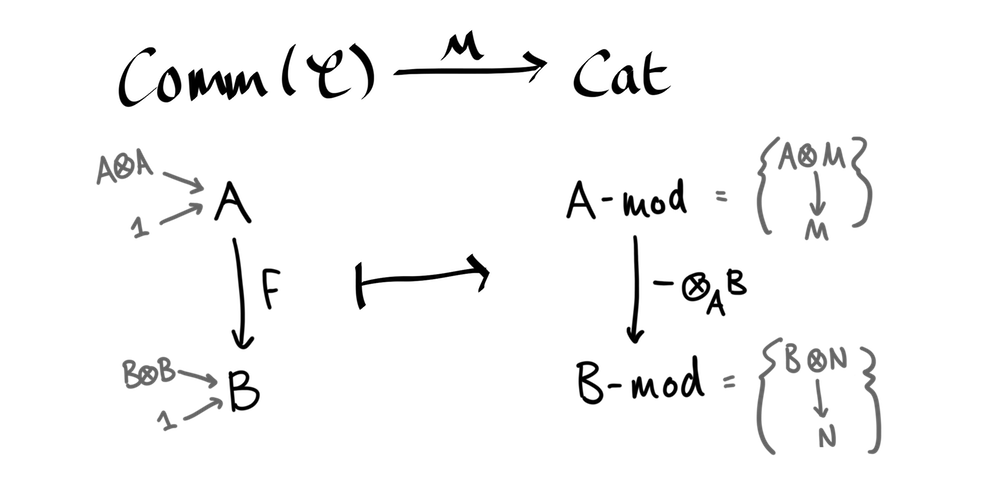
\includegraphics[width=.9\textwidth]{images/MfaithfullyflatwithAmod.png}}
            \caption{Constructing the fpqc topology -- compare with \cref{fg:grothendieckpseudofunctor}}
            \label{fg:MfaithfullyflatwithAmod}
        \end{figure}

        \begin{definition}[Faithfully flat and quasi-compact topology {(Définition~2.8, \S2.2, p.15)}]\label{df:fpqc-topology}
            With definitions as in \cref{eq:m-and-d-for-fpqc}, the $M$-faithfully flat topology on $\aff{\ccat}$ is called the \emph{faithfully flat and quasi-compact} (or simply \emph{fpqc}\footnote{
                In keeping with most current literature, we choose to keep the original French initialism rather than using the English \emph{ffqc}.
            }, or even just \emph{flat}) topology.
        \end{definition}

        \begin{note}[Change of base]\label{nt:change-of-base}
            For a morphism $f\colon X\to Y$ in some category $\dcat$ we have the notion of the \emph{change of base functor $f^*\colon\dcat/Y\to\dcat/X$} given by the pullback along $f$.
            This is \emph{not} quite what we mean when we call $(\blank\otimes_A B)$ a \emph{change of base}.
            We are instead applying the terminology from \cref{df:m-t-grothendieck-setup}: say we have
            \begin{equation*}
                \begin{tikzcd}[row sep=.5em]
                    \spec B \arrow[dr, "p"] &\\
                    & \spec A\\
                    \spec B' \arrow[ur, swap, "q"] &
                \end{tikzcd}
            \end{equation*}
            Then $q_*\colon\modc{B'}\to\modc{A}$ is the forgetful functor, and
            \begin{equation*}
                p^*=(\blank\otimes_A B)\colon\modc{A}\to\modc{B}.
            \end{equation*}
            So $p^*q_*=(\blank\otimes_A B)\colon\modc{B'}\to\modc{B}$ is what we call, in line with \cref{df:m-t-grothendieck-setup}, a change of base.
        \end{note}

        In \cref{sub:the_zariski_topology} we will actually redefine the fpqc topology by spelling out explicitly what it means to be $M$-faithfully flat with $M$ as in \cref{eq:m-and-d-for-fpqc}.
        We do this because it makes it easier to define the \emph{Zariski topology}.
    
    % subsubsection fpqc_topology (end)

% subsection the_faithfully_flat_topology (end)


% !TEX root = ../../../under-spec-z.tex

\subsection{The Zariski topology} % (fold)
\label{sub:the_zariski_topology}

    \emph{Yet again, throughout this section we assume that $\smc$ is a cosmos and use $\dcat$ to refer to an arbitrary category.}

    \subsubsection{Zariski covers} % (fold)
    \label{ssub:zariski_covers}

        Our next goal is to define the \emph{Zariski topology on $\aff{\ccat}$}.
        Once again, we start by defining a certain type of morphism in $\aff{\ccat}$ and saying when a collection of such morphisms gives an \emph{open cover}.

        \begin{definition}[Zariski open {(Définition~2.9,~\S2.3,~p.15)}]\label{df:zariski-open-morphism}
            Let $f\colon A\to B$ in $\comm{\ccat}$.
            Then $f$ is
            \begin{enumerate}[(i)]
                \item \emph{flat} if the functor
                    \begin{equation*}
                        (\blank\otimes_A B)\colon\modc{A}\to\modc{B}
                    \end{equation*}
                    is exact\footnote{
                        We already know that this functor commutes with colimits, since $(\modc{A},\otimes_A,A)$ is closed (\cref{le:modc-a-cosmos-algc-a-bicomplete}), so it is exact if and only if it commutes with finite limits as well, i.e. if and only if it is left exact.
                    };
                \item an \emph{epimorphism} if, for all $X\in\comm{\ccat}$, the map
                    \begin{equation*}
                        (\blank\circ f)\colon\Hom(B,X)\to\Hom(A,X)
                    \end{equation*}
                    is injective;
                \item a \emph{finite presentation} if, for every filtered diagram\footnote{
                        That is, our diagram is \emph{non-empty} and such that
                        \begin{enumerate}[(i)]
                            \item for any two objects $x,y$ in the diagram there exists some object $k$ and arrows \mbox{$x\to k\leftarrow y$};
                            \item for any parallel arrows $f,g\colon x\to y$ there exists some object $k$ and an arrow $a\colon y\to k$ such that $af=ag$.
                        \end{enumerate}
                    } of objects
                    \begin{equation*}
                        \{X_i\in A/\comm{\ccat}\}_{i\in I},
                    \end{equation*}
                    the natural morphism
                    \begin{equation*}
                        \colim_i\Hom_{A/\comm{\ccat}}(B,X_i) \longrightarrow \Hom_{A/\comm{\ccat}}(B,\colim_i X_i)
                    \end{equation*}
                    is an isomorphism.
            \end{enumerate}
            We say that $f\colon\spec B\to\spec A$ in $\aff{\ccat}$ is \emph{Zariski open} (or an \emph{open Zariski immersion}) if the corresponding morphism $f\colon A\to B$ in $\comm{\ccat}$ is a flat epimorphism of finite presentation.
            % (where these three properties are as defined in \cref{tb:flat-epi-finite-presentation}).
        \end{definition}

        % \begin{table}[h!]
        %     \centering
        %     \begin{tabular}{llr}
        %         $f$ is \ldots & if \ldots & is \ldots\\
        %         \toprule
        %         a \emph{flat} morphism & $(\blank\otimes_A B)\colon\modc{A}\to\modc{B}$ & exact\\
        %         an \emph{epimorphism} & $(\blank\circ f)\colon\Hom(B,X)\to\Hom(A,X)$ & injective for all $X$\\
        %         of \emph{finite presentation} & $\spec$ & a
        %     \end{tabular}
        %     \caption{Possible properties of $f\colon A\to B$ in $\comm{\ccat}$}
        %     \label{tb:flat-epi-finite-presentation}
        % \end{table}

        \begin{definition}[fpqc and Zariski covers {(Définition~2.10,~\S2.3,~p.16)}]\label{df:fpqc-zariski-covers}
            A family of morphisms $\{\spec A_i\to\spec A\}_{i\in I}$ in $\aff{\ccat}$ is
            \begin{enumerate}[(i)]
                \item an \emph{fpqc cover} (or simply a \emph{flat cover}) if
                    \begin{enumerate}
                        \item for all $i\in I$, the morphism $\spec A_i\to\spec A$ is flat;
                        \item there exists some finite subset $J\subset I$ such that the functor
                            \begin{equation*}
                                \prod_{j\in J}(\blank\otimes_A A_j)\colon\modc{A}\to\prod_{j\in J}\left(\modc{A_j}\right)
                            \end{equation*}
                            is conservative\footnote{
                                By definition, this is just asking that $(\blank\otimes_A A_j)$ be conservative for each $j\in J$.
                            };
                    \end{enumerate}
                \item a \emph{Zariski cover} if
                    \begin{enumerate}
                        \item it is an fpqc cover;
                        \item for all $i\in I$, the morphism $\spec A_i\to \spec A$ is Zariski open.\qedhere
                    \end{enumerate}
            \end{enumerate}
        \end{definition}

        \emph{We are interested primarily in the Zariski topology, and the fpqc topology will be used essentially only for \elide(\cref{le:essential-image-is-fpqc})} (\S2.3~p.16~\P3).

        \bigskip

        Saying that a family of morphisms is a flat cover, in the sense of the above definition, is just another way\footnote{
            The only real difference between being a flat cover and being $M$-faithfully flat is that the former requires exactness of the change of base functor $(\blank\otimes_A A_i)$ whereas the latter requires only left exactness, but we know that this functor is right exact anyway, since it is left adjoint to the forgetful functor $\modc{A_i}\to\modc{A}$.
            Thus these two requirements coincide.
        } of saying it is $M$-faithfully flat, in the sense of \cref{ssub:fpqc_topology}.
        So we already know that flat covers give rise to a topology: the fpqc (or flat) topology.
        To show that the same is true for Zariski covers we need to show that the property of being Zariski open is preserved by pullbacks and is associative (in the sense of \cref{df:grothendieck-pretopology}), and also that isomorphisms are Zariski open.
        However, \cref{df:zariski-open-morphism} is phrased \emph{not} in terms of $\spec B\to\spec A$, but instead in terms of the corresponding \mbox{$A\to B$}.
        So we need to check that these properties of morphisms of \emph{commutative monoids} are stable under \emph{pushouts}.
        Stability of finite presentation follows from a lengthy definition chase, and epimorphisms are always stable under pushouts\footnote{
             \cite[Proposition~2.5.3(1)]{Borceux:1994ws}
        }.
        As for flatness, the fpqc topology already tells us that flatness is preserved.

        \begin{definition}[Zariski topology]
            The topology on $\aff{\ccat}$ generated\footnote{
                As in \cref{le:m-t-grothendieck-pretopology}.
            } by Zariski covers is called the \emph{Zariski topology}.
        \end{definition}

        \begin{note}
            Because we require both fpqc and Zariski covers to be finitely conservative, a sieve $S$ on $\spec A$ is in the generated topology if and only if it contains some cover if and only if it contains the finite conservative subset of that cover.
            This means that these pretopologies are \emph{quasi-compact}, i.e. generated by finite covering families.
            For more, see the beginning of \cite[\S~IX.11]{MacLane:1992uz}.
        \end{note}
        
    % subsubsection zariski_covers (end)


    \subsubsection{Sheaves} % (fold)
    \label{ssub:sheaves}

        Just as in classical algebraic geometry, now that we have some topology we can introduce the idea of `gluing together' affine schemes to obtain \emph{schemes}.
        Fundamental to this idea is the definition of a \emph{sheaf}.

        \begin{definition}[Sheaves on a site]\label{df:sheaves-on-site}
            Let $(\dcat,J)$ be a site\footnote{
                \cref{df:site}
            } and $F\in\PShv(\dcat)$ some presheaf\footnote{
                \cref{df:presheaves}
            }.
            We say that $F$ is a \emph{$J$-sheaf} (or simply a \emph{sheaf} if the context is clear) if, for all objects $X\in\dcat$ and covering sieves $S\in J(X)$ on $X$, the natural map
            \begin{equation*}
                \Hom(\Hom(\blank, X), F)\longrightarrow\Hom(S,F)
            \end{equation*}
            induced by the inclusion $S\hookrightarrow\Hom(\blank, X)$ is a bijection.

            We write $\Shv^J(\dcat)$ to be the category of sheaves on $(\dcat,J)$, a full subcategory of $\PShv(\dcat)$.
        \end{definition}

        If we have a pretopology then we can rewrite this definition in a way which is sometimes easier to apply in practice, and also gives a better geometric intuition.

        \begin{lemma}[Sheaves on a presite]\label{le:sheaves-on-presite}
            Let $(\dcat, C)$ be a presite\footnote{
                This is not standard terminology, but we define a \emph{presite} as a pair $(\dcat,C)$ consisting of a category $\dcat$ and a Grothendieck pretopology $C$ on $\dcat$.
                Given such a pair, we can talk about the \emph{site that it generates} by endowing $\dcat$ with the Grothendieck topology generated by $C$.
            }, $(\dcat, J)$ the site that it generates, and $F\in\PShv(\dcat)$.
            Then $F\in\Shv^{J}(\dcat)$ if and only if, for all objects $X\in\dcat$ and covering families $\{X_i\to X\}_{i\in I}\in C(X)$ of $X$,
            \begin{equation*}
                F(X) = \eq\left( \prod_{i\in I}F(X_i)\rightrightarrows\prod_{j,k\in I}F(X_j\times_X X_k) \right)
            \end{equation*}
            (where the \emph{equaliser} $\eq$ is the dual notion to the coequaliser\footnote{
                \cref{df:coequaliser}
            }).
        \end{lemma}

        \begin{proof}
            \cite[\S III.4,~Proposition 1]{MacLane:1992uz}
        \end{proof}

        As for how this provides us with some intuition, let us return to the example of $\Op{T}$.
        In this category, pullbacks correspond to intersection, and we think of presheaves as being functions on the open sets that take inclusion maps to restriction maps.
        \cref{le:sheaves-on-presite} says that $F$ is a sheaf if and only if, when we piece together all of the $F(X_i)$ that agree on overlaps (this is the equaliser term), we get exactly $F(X)$, for any cover ${X_i}$ of $X$.
        This is just the (classical) presheaf condition -- see \cref{fg:sheaves}.
        % Then the equaliser condition in \cref{le:sheaves-on-presite} says that a presheaf $F$ is a sheaf if and only if, for all open sets $X$ and all Zariski open covers\footnote{
            % Here we would need to unpack some definitions: this doesn't have to hold for \emph{any} open cover $\{X_i\}$ of $X$; it only has to hold for Zariski covers (\cref{df:fpqc-zariski-covers}).
        % } $\{X_i\}$ of $X$,
        % \begin{equation*}
            % \left(F\big|_{X_i}\right)\bigg|_{X_i\cap X_j} = \left(F\big|_{X_j}\right)\bigg|_{X_i\cap X_j}
        % \end{equation*}
        % which coincides with our classical intuition of what a sheaf should be.

        \begin{figure}[h]
            \centering
            \frame{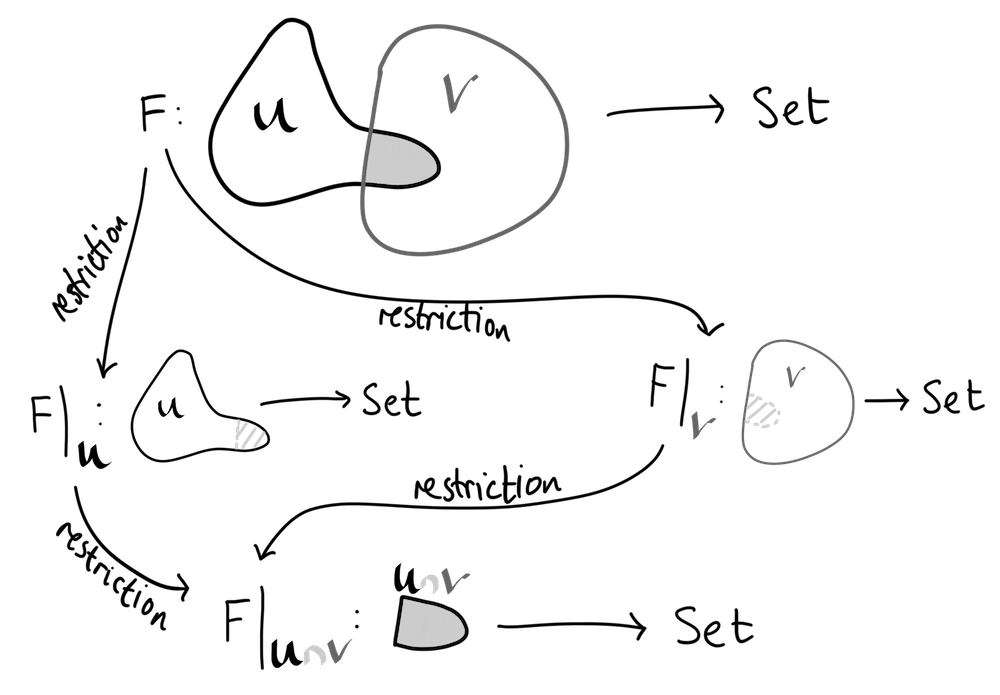
\includegraphics[width=.85\textwidth]{images/sheaves.png}}
            \caption{The fact that we always have a morphism from $F(X)$ to the equaliser in \cref{le:sheaves-on-presite} corresponds to the classical presheaf condition: for presheaves on a topological space it doesn't matter whether we restrict $U\cup V$ to $U\cap V$ via $U$ or via $V$}
            \label{fg:sheaves}
        \end{figure}

        \bigskip

        Since the Zariski topology is coarser (see \cref{fg:zariski-vs-fpqc-topology}) than the fpqc topology, the collection of fpqc covering sieves on some object is at least as large as the collection of Zariski covering sieves.
        This means that asking for the map induced by inclusion in \cref{df:sheaves-on-site} to be a bijection for all covering sieves on an object is a stricter condition in the fpqc topology than in the Zariski topology.
        So being an fpqc sheaf implies being a Zariski sheaf, but the converse doesn't necessarily hold.
        Thus we have the subcategories
        \begin{equation*}
            \Shv^{\text{fpqc}}(\aff{\ccat})\subset\Shv^{\text{Zar}}(\aff{\ccat})\subset\PShv(\aff{\ccat}).
        \end{equation*}

        \begin{note}
            As already stated, our primary interest is the Zariski topology, so whenever we speak of sheaves without reference to a specific topology it is assumed that we mean Zariski sheaves.
            Similarly, we write $\Shv(\aff{\ccat})=\Shv^{\text{Zar}}(\aff{\ccat})$.
        \end{note}

        \begin{figure}[h]
            \centering
            \frame{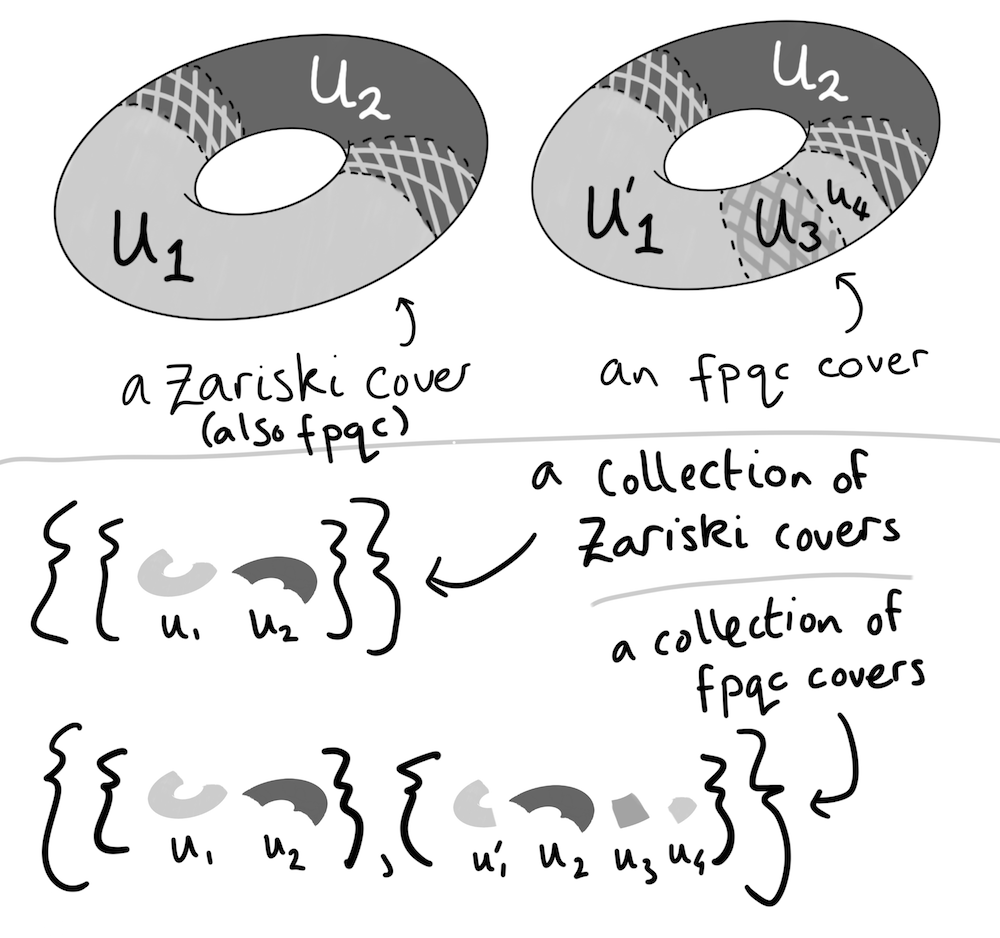
\includegraphics[width=.8\textwidth]{images/zariski-vs-fpqc-topologyNEW.png}}
            % \caption{Two topologies $\sigma,\tau$; here $\tau$ is coarser than $\sigma$}
            \caption{The Zariski topology is \emph{coarser} than the fpqc topology, i.e. it has fewer open sets, so every Zariski cover is also an fpqc cover -- the sheaf condition `reverses' this inclusion: there are \emph{more} fpqc covers than Zariski, hence \emph{fewer} fpqc sheaves than Zariski (and \textbf{maybe} hence \emph{more} fpqc schemes (something we don't define) than Zariski; see \cref{fg:hierarchy} for a similar conjecture)}\label{fg:zariski-vs-fpqc-topology}
        \end{figure}

        In \cref{ssub:motivating_example} we identified $\aff{k}$ with its essential image in $\PShv(\aff{k})$ under the Yoneda embedding, and we can do the same here: identify $\aff{\ccat}$ with its essential image in $\PShv(\aff{\ccat})$ under the Yoneda embedding.
        It turns out, however, that we can actually come up with a stronger result.

        \begin{lemma}[\mbox{}{(Corollaire~2.11,~\S2.3,~p.17)}]\label{le:essential-image-is-fpqc}
            For all $X\in\aff{\ccat}$ the presheaf $Y_X$ coming from the Yoneda embedding\footnote{
                \cref{le:yoneda-lemma,le:yoneda-embedding}
            } is an fpqc sheaf.
        \end{lemma}

        \begin{proof}
            The proof in \cite{Toen:2005wxa} uses stacks; see \cref{nt:no-theorem-2.5}.
        \end{proof}

        Firstly, this exactly says that the fpqc topology (and thus the Zariski topology, since it is coarser) is \emph{subcanonical}: all representable presheaves are fpqc sheaves.
        Secondly, this means we have the equivalence of categories
        \begin{equation}\label{eq:both-types-of-affine-schemes}
            \aff{\ccat}\equiv\ASch(\ccat) 
        \end{equation}
        where we define the full subcategory $\ASch(\ccat)\subset\Shv(\aff{\ccat})$ by
        \begin{equation*}
            \ASch(\ccat)=\{X\in\Shv(\aff{\ccat}) \mid X\cong \Hom_{\aff{\ccat}}(\blank,\spec A)\text{ for some } \spec A\in\aff{\ccat}\}.
        \end{equation*}
        We call the objects of $\ASch(\ccat)$ \emph{affine schemes}.
        
        \begin{definition}[Affine schemes over $\ccat$]\label{df:affine-schemes-general}
            From now on we use the phrase `affine scheme' interchangeably, to mean an object of either $\aff{\ccat}$ or $\ASch(\ccat)$.
            We often use the same notation for both as well (so for $\spec A\in\aff{\ccat}$ we also write $\spec A\in\ASch(\ccat)$ to mean $Y_A=\Hom(\blank,\spec A)$, and vice versa).
        \end{definition}
        
    % subsubsection sheaves (end)

% subsection the_zariski_topology (end)








    \clearpage


% !TEX root = ../../../under-spec-z.tex

\subsection{Schemes} % (fold)
\label{sub:schemes}

    % \vspace{-2em}
    % \begin{translation}{2.4}{1}
    %     In this section we present the main definition of this paper, that of a \emph{scheme over $\ccat$}.
    %     For this, we start by introducing the idea of an open Zariski cover in $\Shv(\aff{\ccat})$, and will define schemes as sheaves possessing an open Zariski cover of affine schemes.
    %     We will then demonstrate some fundamental properties of schemes (for example, gluing, and stability under pullbacks and disjoint unions).
    % \end{translation}

    \begin{quotation}
        \emph{In this section we present the main definition of this paper, that of a \emph{scheme over $\ccat$}.} (\S2.4,~\P1)
    \end{quotation}

    \subsubsection{Using sheaves} % (fold)
    \label{ssub:using_sheaves}

        % At the end of \cref{sub:the_zariski_topology} we showed how we can consider the category $\aff{\ccat}$ of affine schemes as being embedded inside $\Shv^{\text{fpqc}}(\aff{\ccat})$, and then slightly broaden our definition of affine schemes to include any (Zariski) sheaf in the essential image of this embedding (that is, close the collection of affine schemes under isomorphism).
        % \Cref{df:zariski-open-morphism,df:fpqc-zariski-covers} define what it means for a morphism of affine schemes \emph{as objects of $\aff{\ccat}=\op{\comm{\ccat}}$} to be Zariski open, but we should now give equivalent conditions for when a morphism of affine schemes \emph{as objects of $\ASch(\ccat)$} is Zariski open.
        % We use \cref{df:zariski-open-sheaves} as our temporary definition for this latter scenario, and then prove that it is equivalent to our previous definition in \cref{le:zariski-open-sheaves-and-morphisms}.

        In light of \cref{eq:both-types-of-affine-schemes}, we need to rephrase \cref{df:zariski-open-morphism,df:fpqc-zariski-covers} in terms of sheaves.

        \begin{definition}[Zariski open in {$\Shv(\aff{\ccat})$} {(Définition~2.12,~\S2.4,~p.18)}]\label{df:zariski-open-sheaves}
            \mbox{}\vspace{-1em}
            \begin{enumerate}[(i)]
                \item Let $X\in\ASch(\ccat)$ and $F\subset X$ a subsheaf of $X$.
                    We say that $F$ is \emph{Zariski open in $X$} if there exists a Zariski-open (in the sense of \cref{df:zariski-open-morphism}\footnote{
                        Recall \cref{df:affine-schemes-general}: $X$ is not necessarily in $\aff{\ccat}$, but we know that we can find some $\spec B\in\aff{\ccat}$ such that $X\cong\Hom(\blank,\spec B)$.
                        Similarly we can find $\spec B_i\in\aff{\ccat}$ such that $X_i\cong\Hom(\blank,\spec B_i)$.
                        Then we want the family $\{\spec B_i\to\spec B\}_{i\in I}$ to be Zariski open in the sense of \cref{df:zariski-open-morphism}.
                    }) family $\{X_i\to X\}_{i\in I}$ in $\aff{\ccat}$ (where $I$ is \emph{not} necessarily finite\footnote{
                        See the paragraph accompanying \cref{fg:infinitely-many-lines,fg:disjointlines}, just before \cref{ssub:partial_summary}.
                    }) and a sheaf morphism $\coprod_{i\in I}X_i\to X$ whose image in $X$ is $F$.
                \item A morphism $f\colon F\to G$ in $\Shv(\aff{\ccat})$ is \emph{Zariski open} (or an \emph{open Zariski immersion}) if, for all affine schemes $X$ and morphisms $X\to G$, the induced morphism
                \begin{equation*}
                    F\times_G X\to X
                \end{equation*}
                is a monomorphism whose image is Zariski open in $X$.\qedhere
            \end{enumerate}
        \end{definition}

        By definition, Zariski-open morphisms are stable under a change of base and also under composition in $\Shv(\aff{\ccat})$.
        Further, \emph{it can be easily checked that Zariski-open morphisms are monomorphisms in $\Shv(\aff{\ccat})$.} (\S2.4,~\P2)
        When we introduce schemes we will see that this point about monomorphisms is an example of a property holding on all affine schemes in a cover implying that the same property holds for the whole scheme, i.e. `locally a monomorphism implies globally a monomorphism'.

        \bigskip

        At the moment we have two definitions for what it means for a morphism of affine schemes to be Zariski open: \cref{df:zariski-open-morphism} for $\aff{\ccat}$; and \cref{df:zariski-open-sheaves} for $\ASch(\ccat)$.
        The following lemma shows that the two definitions are indeed equivalent.

        \begin{lemma}[\mbox{}{Lemme~2.14,~\S2.4,~p.18}]\label{le:zariski-open-sheaves-and-morphisms}
            Let $f\colon Z\to Y$ be a morphism of affine schemes.
            Then $f$ is Zariski open in the sense of \cref{df:zariski-open-morphism} if and only if it is Zariski open in the sense of \cref{df:zariski-open-sheaves}.
        \end{lemma}

        \begin{proof}
            This proof is largely unpacking definitions, and is given in \cite{Toen:2005wxa}.
        \end{proof}

        \begin{definition}[Scheme relative to $\ccat$ {(Définition~2.15,~\S2.4,~p.19)}]\label{df:relative-scheme}
            A sheaf $F\in\Shv(\aff{\ccat})$ is a \emph{scheme relative to $\ccat$} (or simply a \emph{scheme} if the context is clear) if there exists a family $\{X_i\}_{i\in I}$ of affine schemes and a morphism
            \begin{equation*}
                p\colon\left(\coprod_{i\in I}X_i\right)\to F
            \end{equation*}
            satisfying the following two conditions:
            \begin{enumerate}[(i)]
                \item $p$ is an epimorphism of sheaves;
                \item for all $i\in I$ the morphism\footnote{
                    That is, the induced morphism $X_i\to\coprod X_i\to F$.
                } $X_i\to F$ is an open Zariski immersion.
            \end{enumerate}
            We define the category $\Sch(\ccat)$ to be the full subcategory of $\Shv(\aff{\ccat})$ consisting of such sheaves, and call the family $\{X_i\to X\}$ an \mbox{\emph{affine Zariski cover of $F$}}.
        \end{definition}

        At the moment, we simply know that a scheme is in some sense `covered' by affine schemes -- we do not yet know exactly how these affine schemes `fit together' (we find out in \cref{le:actual-gluing}).
    
        \begin{figure}[h]
            \centering
            \frame{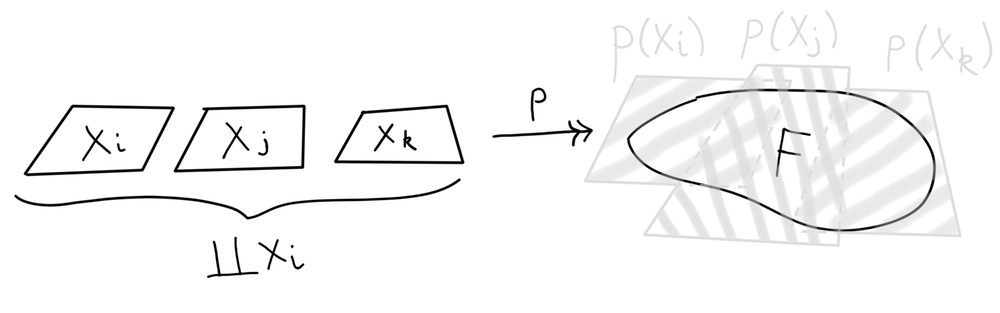
\includegraphics[width=\textwidth]{images/scheme.png}}
            \caption{\Cref{df:relative-scheme} -- schemes}
            \label{fg:scheme}
        \end{figure}

        When we defined Zariski covers in \cref{df:fpqc-zariski-covers} we required them to be finitely conservative, but here we don't have any finiteness conditions -- we use the word `cover' in two slightly different senses.
        Here it is not so much a topological cover, as a scheme-theoretic cover.
        Locally, schemes `look like' affine schemes, which have this finitely conservative (i.e. \emph{quasi-compact}) property, but globally they are not under such tight restrictions.
        See \cref{fg:infinitely-many-lines,fg:disjointlines}.

        \begin{figure}[h]
            \begin{minipage}{0.48\textwidth}
                \centering
                \frame{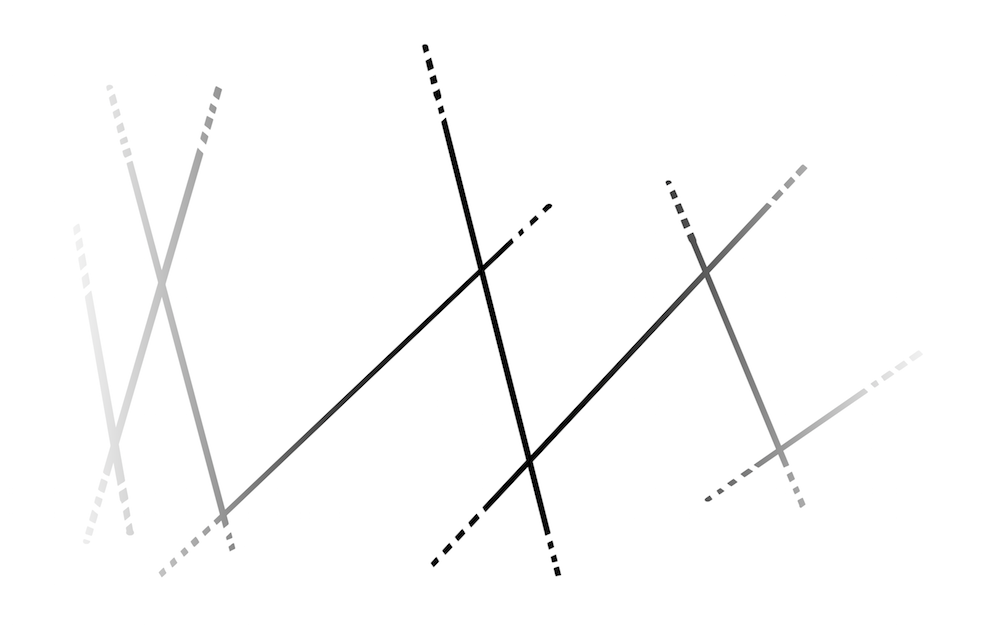
\includegraphics[width=\textwidth]{images/infinitely-many-lines.png}}
                \caption{Consider infinitely many lines glued together pairwise at a point -- this is a scheme, since we can take the $X_i$ to be the lines, then $\{X_i\}$ is an \emph{infinite} affine Zariski cover}
                \label{fg:infinitely-many-lines}
            \end{minipage}
            \hfill
            \begin{minipage}{0.45\textwidth}
                \centering
                \frame{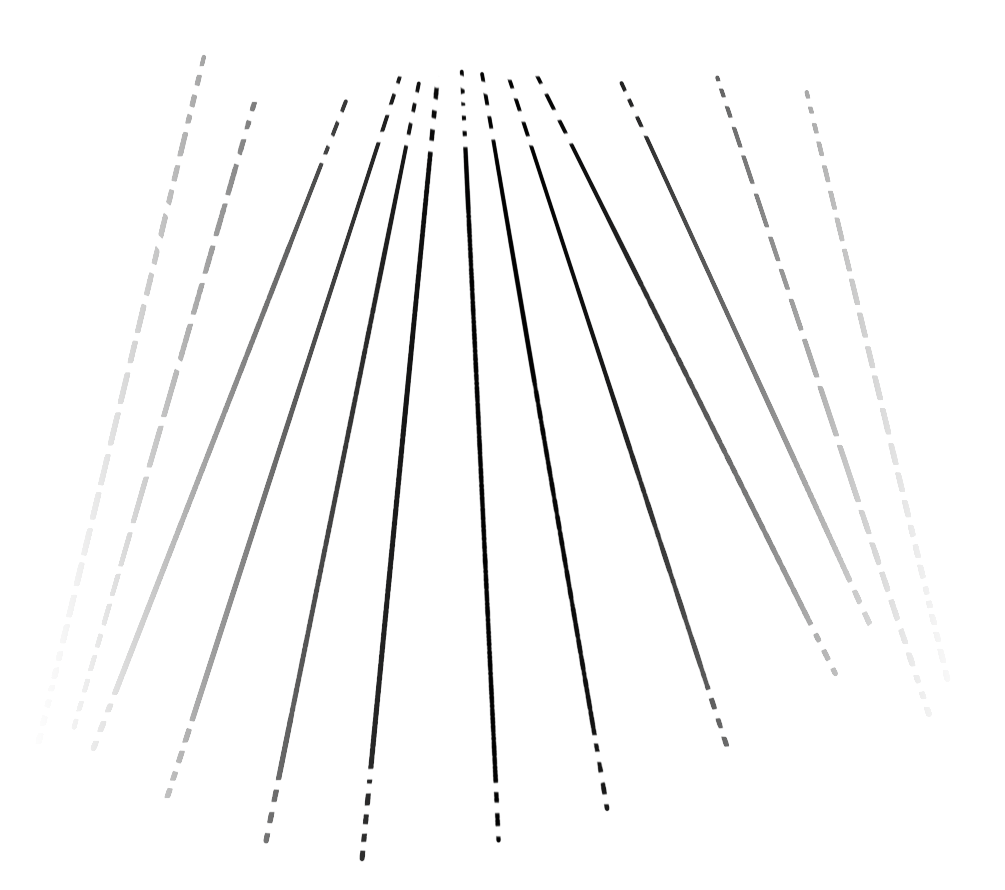
\includegraphics[width=\textwidth]{images/disjointlines.png}}
                \caption{The trivial gluing (coproduct) of infinitely many lines; here we can take the $X_i$ to be the lines and $p$ to simply be the identity}
                \label{fg:disjointlines}
            \end{minipage}
        \end{figure}

    % subsubsection using_sheaves (end)




    \subsubsection{Partial summary} % (fold)
    \label{ssub:partial_summary}

        Before moving on to talk about the properties schemes, we provide a brief summary of what we have done so far.

        In \cref{ssub:zariski_covers} we defined two topologies on $\aff{\ccat}=\op{\comm{\ccat}}$ by defining certain types of \emph{open} morphisms: \emph{fpqc} and \emph{Zariski}.
        After this, in \cref{ssub:sheaves}, we looked at a more abstract situation: using the topologies we just defined to consider fpqc and Zariski \emph{sheaves}\footnote{
            Then agreeing, from now on, to say \emph{sheaf} to mean a \emph{Zariski} sheaf.
        }.
        Then, with the Yoneda embedding, we considered $\aff{\ccat}$ as sitting inside $\Shv^\text{fpqc}(\aff{\ccat})\subset\PShv(\aff{\ccat})$, and called the essential image of this embedding $\ASch(\ccat)$, whose objects are \emph{affine schemes}.
        % \begin{equation}\label{eq:diagram-of-inclusions}
        %     \begin{array}{ccccccccc}
        %         & & &\tightoverset{close under isomorphism}{\big\downarrow} & & & &\tightoverset{ignore topology (coarser)}{\big\downarrow} &\\
        %         \aff{\ccat} &\hookrightarrow &\Shv^{\text{fpqc}}(\aff{\ccat}) &\subset &\ASch(\ccat) &\subset &\Shv(\aff{\ccat}) &\subset &\PShv(\aff{\ccat})\\
        %         &\tightunderset{Yoneda functor}{\big\uparrow} & & & &\tightunderset{pass to Zariski topology}{\big\uparrow} & & &
        %     \end{array}
        % \end{equation}
        Next, in \cref{df:zariski-open-sheaves}, we extended our definition of Zariski open morphisms to general sheaf morphisms and showed that it agreed with our previous definition.
        We used this to define a \emph{scheme} as a sheaf that was covered by affine schemes, with each affine scheme embedding into the sheaf via a Zariski open immersion.
        By definition, every affine scheme is also a scheme (just as we would expect) and every scheme is a sheaf.
        \Cref{fg:hierarchy} shows how all these full subcategories overlap inside $\PShv(\aff{\ccat})$.
    
        \begin{figure}[h!]
            \centering
            \begin{minipage}[t]{0.65\textwidth}
                \vspace{0pt}
                \frame{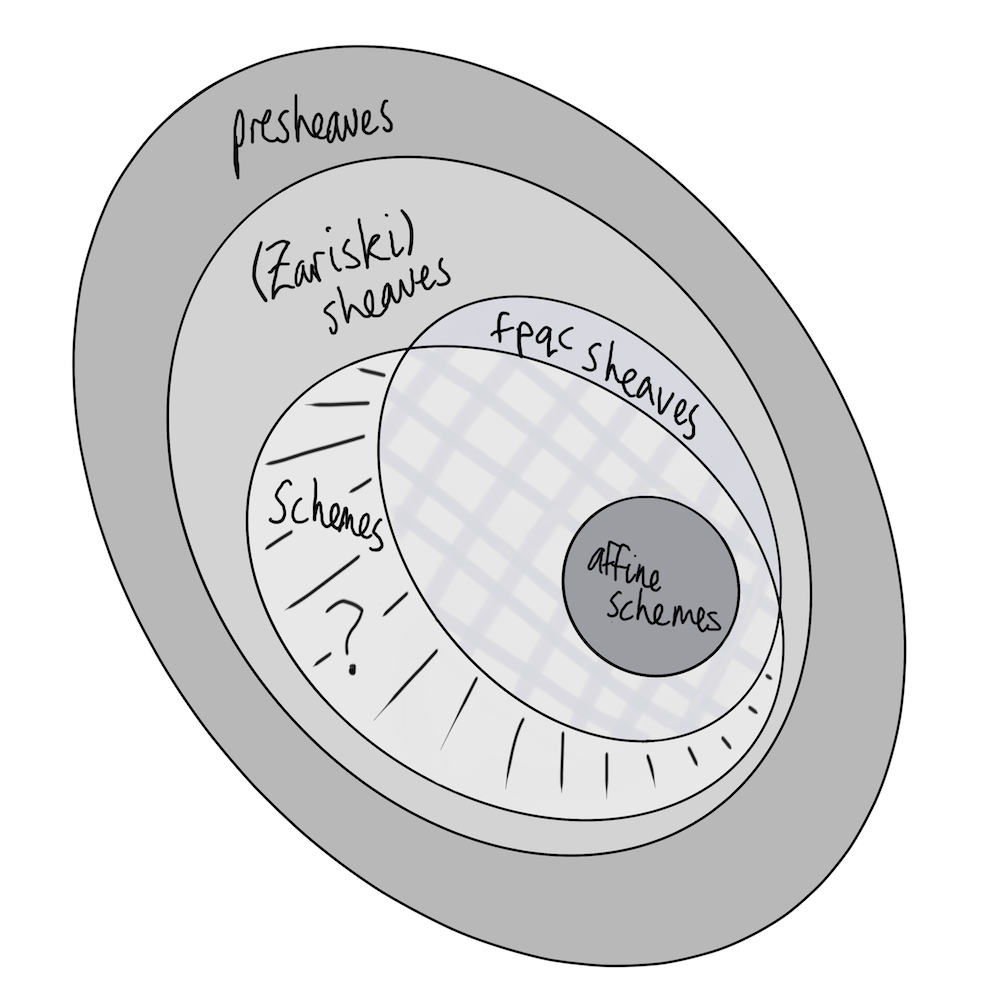
\includegraphics[width=\textwidth]{images/hierarchy.png}}
            \end{minipage}
            \hfill
            \begin{minipage}[t]{0.33\textwidth}
                \vspace{0pt}
                \caption{The hierarchy, considering objects up to isomorphism -- really there are `lots more' fpqc sheaves than schemes: $\Shv^{\text{fpqc}}(\aff{\ccat})$ is bicomplete but $\Sch(\ccat)$ does \emph{not} have all colimits, so we can construct $X\in\Shv^{\text{fpqc}}(\aff{\ccat})\setminus\Sch(\ccat)$ by talking a sufficiently nasty colimit\\\textbf{Note:} it seems possible (hence the question mark) that $\Sch(\ccat)\subset\Shv^\text{fpqc}(\aff{\ccat})$, since Zariski open morphisms are also flat morphisms, and we have an `fpqc-sheafification' functor $\Shv(\aff{\ccat})\to\Shv^\text{fpqc}(\aff{\ccat})$ that is a left adjoint (and so preserves colimits) -- this is not mentioned in \cite{Toen:2005wxa} and we don't have the space here to go any further}\label{fg:hierarchy}
            \end{minipage}
        \end{figure}

        % \begin{equation*}\label{eq:full-diagram-of-inclusions}
        %     \begin{array}{ccccccccccc}
        %         & &\tightoverset{fpqc sheaves}{\big\downarrow} & & & &\tightoverset{schemes}{\big\downarrow} & & & &\tightoverset{presheaves}{\big\downarrow}\\
        %         \aff{\ccat} &\twoheadrightarrow &\Shv^{\text{fpqc}}(\aff{\ccat}) &\subset &\ASch(\ccat) &\subset &\Sch(\ccat) &\subset&\Shv(\aff{\ccat}) &\subset &\PShv(\aff{\ccat}).\\
        %         \tightunderset{affine schemes}{\big\uparrow} & & & &\tightunderset{affine schemes}{\big\uparrow} & & & &\tightunderset{(Zariski) sheaves}{\big\uparrow} & &
        %     \end{array}
        % \end{equation*}
        


    % subsubsection partial_summary (end)



    \subsubsection{Properties of schemes} % (fold)
    \label{ssub:properties_of_schemes}

        We now state some fundamental properties of schemes, and refer the reader to \cite{Toen:2005wxa} for proofs of each one.
        However, there are diagrams (at the end of this section) of sketches for most of the proofs, which should hopefully convey the main ideas reasonably well.
        The conventions used in these diagrams is explained in \cref{fg:diagram-key}.
        We recall that we can think of pullbacks as a generalisation of fibres; that pullbacks of epimorphisms are epimorphisms; and that pullbacks of Zariski open morphisms are Zariski open.
        
        % \begin{figure}[h]
        %     \floatbox[{\capbeside\thisfloatsetup{capbesideposition={right,top},capbesidewidth=4.5cm}}]{figure}[\FBwidth]
        %     {\caption{The diagram corresponding to the statement `if a sheaf $F$ has an affine Zariski cover $\{A_i\}$ then it is a scheme' -- the lighter grey corresponds to the hypotheses on $F$ -- note that we don't have any notation for whether or not a map is Zariski open, in an attempt to retain simplicity}\label{fg:example-diagram}}
        %     {\frame{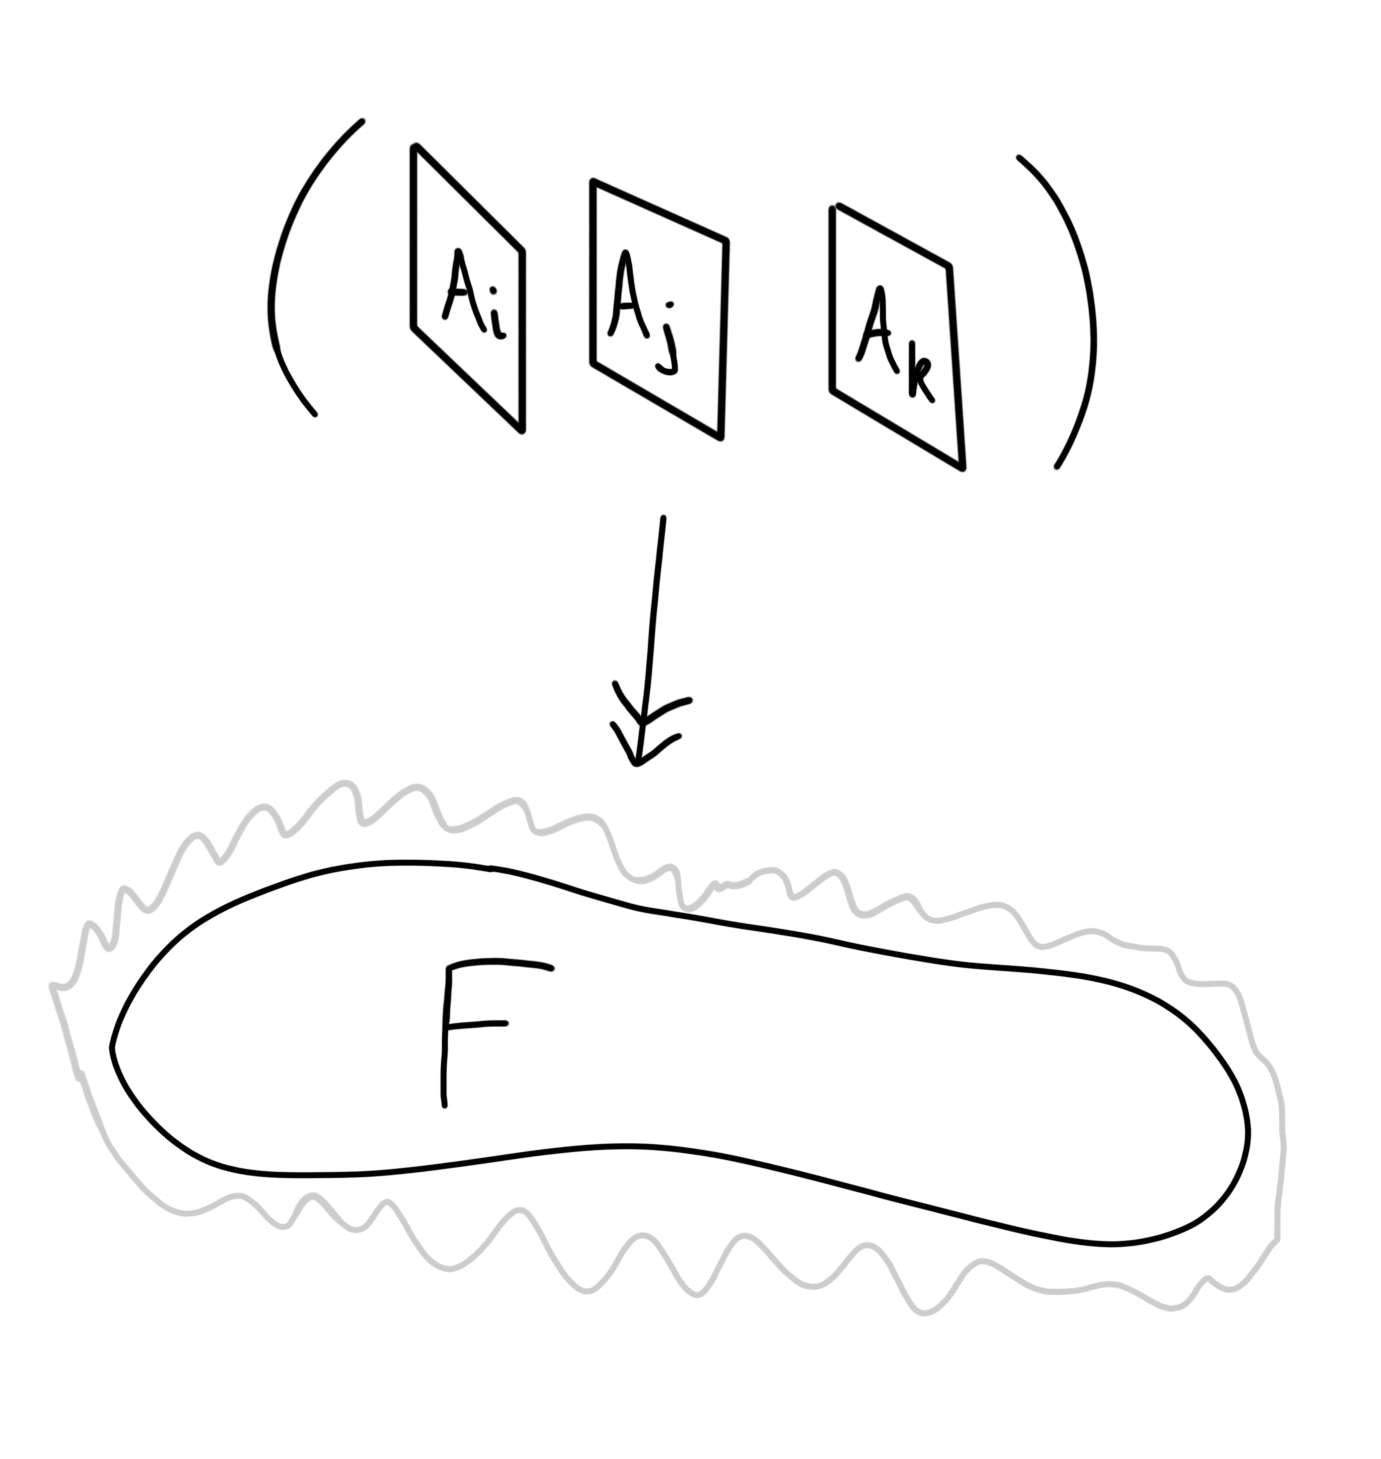
\includegraphics[width=.4\textwidth]{images/example-diagram.png}}}
        % \end{figure}

        % A fundamental property of relative schemes is that of \emph{recollement}.

        \begin{lemma}[Gluing and affine schemes {(Proposition~2.6,~\S2.4,~p.20)}]\label{le:recollement-and-affine}
            \mbox{}\vspace{-1em}
            \begin{enumerate}[(i)]
                \item Let $A,B$ be affine schemes, $G$ a sheaf, and $G\to A\leftarrow B$ morphisms of sheaves.
                    If $G$ is a scheme then $F=B\times_A G$ is also a scheme.
                \item Let $A$ be an affine scheme, $F$ a sheaf, and $F\to A$ a morphism of sheaves.
                    If there exists an affine Zariski cover $\{A_i\to A\}$ such that each $F\times_A A_i$ is a scheme then $F$ is a scheme.\qedhere
            \end{enumerate}
        \end{lemma}

        % \begin{proof}
        %     See \cite{Toen:2005wxa}.
        % \end{proof}

        % We now note a few more useful properties of schemes that follow from what we have so far, pausing along the way only to make another category theoretical definition.







        \clearpage






        \begin{lemma}[\mbox{}{Proposition~2.17,~\S2.4,~p.21}]
            \mbox{}\vspace{-1em}
            \begin{enumerate}[(i)]
                \item Let $F$ be a scheme and $F_0\subset F$ be Zariski open in the sense of \cref{df:zariski-open-sheaves}.
                    Then $F_0$ is a scheme.
                \item Let $f\colon F\to G$ be a morphism between schemes.
                    Then $f$ is Zariski open in the sense of \cref{df:zariski-open-sheaves} if and only if $f$ satisfies the following two conditions:
                    \begin{enumerate}
                        \item $f$ is a monomorphism;
                        \item there exists an affine Zariski cover $\{X_i\to F\}$ such that each morphism $X_i\to G$ given by composition with $f$ is Zariski open.\qedhere
                    \end{enumerate}
            \end{enumerate}
        \end{lemma}

        % \begin{proof}
        %     See \cite{Toen:2005wxa}.
        % \end{proof}

        % Before the next lemma, which lets us think of a scheme as being glued together from affine schemes, we give a rough definition of a \emph{congruence on an object}, and refer the reader to \cite{Anonymous:_jtXUz4d} for precise details.

        \begin{definition}[Congruence on an object]
            For $X\in\dcat$, a congruence $R$ on $X$ is\footnote{
                Up to some notion of isomorphism between morphisms -- see \cite{Anonymous:_jtXUz4d}.
            } a monomorphism
            \begin{equation*}
                R\overset{(p_1,p_2)}{\hookrightarrow} X\times X
            \end{equation*}
            equipped with the following morphisms:
            \begin{enumerate}[(i)]
                \item (\emph{reflexivity}) $r\colon X\to R$ such that $p_1\circ r=p_2\circ r=\id_X$;
                \item (\emph{symmetry}) $s\colon R\to R$ such that $p_1\circ s=p_2$ and $p_2\circ s=p_1$;
                \item (\emph{transitivity}) $t\colon R\times_X R\to R$ such that
                    \begin{equation*}
                        \begin{tikzcd}[column sep=2em, row sep=2.5em]
                            R\times_X R \arrow[r, swap, "\pi_1"] \arrow[r, bend left=50, "t"] \arrow[d, "\pi_2"] \arrow[d, bend right=50, swap, "t"] & R \arrow[d, "p_1"]\\
                            R \arrow[r, swap, "p_2"] & X
                        \end{tikzcd}
                    \end{equation*}
                    commutes (where $\pi_1$, $\pi_2$ are the pullback morphisms).
            \end{enumerate}
            Given such an $R$, we define the \emph{quotient object $X/R$} as
            \begin{equation*}
                X/R=\coeq(R\overset{p_1}{\underset{p_2}{\rightrightarrows}} X).\qedhere
            \end{equation*}
        \end{definition}


        \begin{lemma}[Stability; gluing affine schemes {(Proposition~2.18,~\S2.4,~p.21)}]\label{le:actual-gluing}
            \mbox{}\vspace{-1em}
            \begin{enumerate}[(i)]
                \item The subcategory $\Sch(\ccat)\subset\Shv(\aff{\ccat})$ is stable under disjoint unions and pullbacks.
                \item A sheaf $F\in\Shv(\aff{\ccat})$ is a scheme if and only if there exists some congruence $R$ on some sheaf $X\in\Shv(\aff{\ccat})$ where the following four conditions are satisfied:
                \begin{enumerate}
                    \item $X\cong\coprod_{i\in I}U_i$ for some affine schemes $U_i$;
                    \item for all $(i,j)\in I^2$, the subsheaf $R_{i,j}\subset U_i\times U_j$ given by the pullback\footnote{
                        `Intersecting down' the congruence: $R\cong\coprod_{i,j}R_{i,j}$.
                        The morphisms $U_i\times U_j\to X\times X$ are those induced by the $U_i\to\coprod U_i\congto X$.
                    }
                        \begin{equation*}
                            \begin{tikzcd}[column sep=1em]
                                R_{i,j} \arrow[r] \arrow[d] & U_i\times U_j \arrow[d]\\
                                R \arrow[r] & X\times X
                            \end{tikzcd}
                        \end{equation*}
                        is such that each induced morphism
                        \begin{equation*}
                            R_{i,j}\to U_i
                        \end{equation*}
                        is Zariski open;
                    \item for each $i\in I$ the subobject $R_{i,i}\subset U_i\times U_i$ is equal to the image of the diagonal morphism $U_i\to U_i\times U_i$;
                    \item $F\cong X/R$.\qedhere
                \end{enumerate}
            \end{enumerate}
        \end{lemma}

        % \begin{proof}
        %     See \cite{Toen:2005wxa}.
        % \end{proof}

        % The reason that this lemma is so important is because it confirms our hope that schemes are `affine schemes glued together in a nice way'.
        % Part (i) says that if we place two schemes side-by-side (i.e. trivially glue them) or `intersect' (\textbf{TJH again, is `intersect' the right word here?}) them, then the result is also a scheme.
        % Part (ii) says that a scheme is exactly what we get if we take some affine schemes $U_i$ with affine subschemes $V_i\subset U_i$ such that the inclusion is Zariksi open, and identify some $V_j$ with $V_i$ in a suitably nice way.
        It is possible to rephrase \cref{le:actual-gluing}(ii) in terms of pushouts.
        Say we have affine schemes $A,X,Y$ and Zariski-open immersions $A\to X$, $A\to Y$.
        Then $X\coprod_A Y$ is the presheaf obtained by gluing $X$ and $Y$ along the images of $A$ (see \cref{fg:gluing}).
        The above lemma then says that this presheaf is also actually a scheme.

        % \begin{figure}[h!]
        %     \centering
        %     \frame{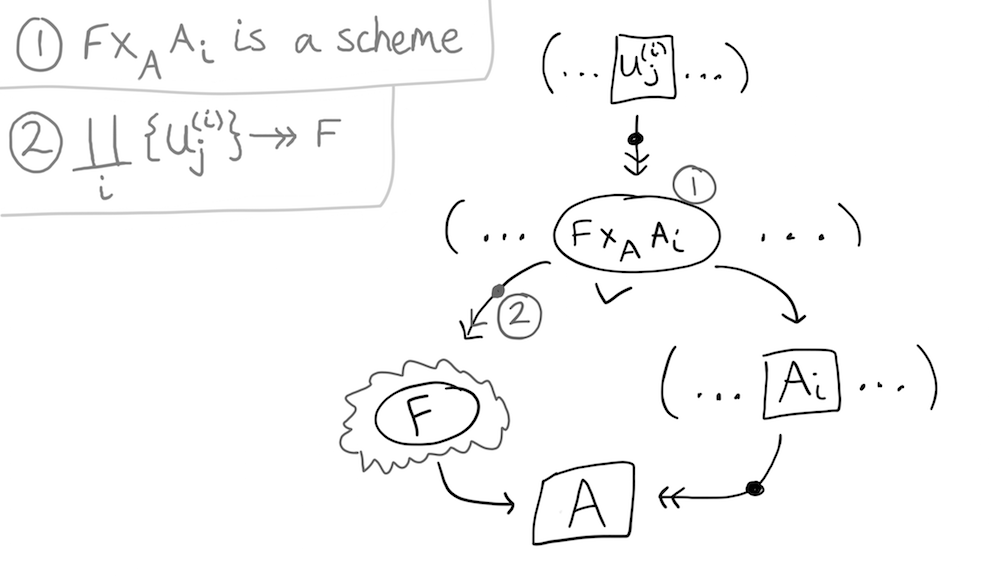
\includegraphics[width=\textwidth]{images/recollement-affine-ii-new.png}}
        %     \caption{\cref{le:recollement-and-affine}(ii) -- \emph{this lemma is a special case of \cite[Lemme~2.20,~\S2.4]{Toen:2005wxa}} -- for \numberincircle{1} the previous part of the lemma tells us that \mbox{$F\times_A A_i$} is a scheme; \numberincircle{2} says that if we take affine covers for all of the \mbox{$F\times_A A_i$} then together they cover $F$}\label{fg:recollement-affine-ii}
        % \end{figure}

        % \begin{figure}[h!]
        %     \centering
        %     \begin{minipage}[t]{0.4\textwidth}
        %         \vspace{0pt}
        %         \frame{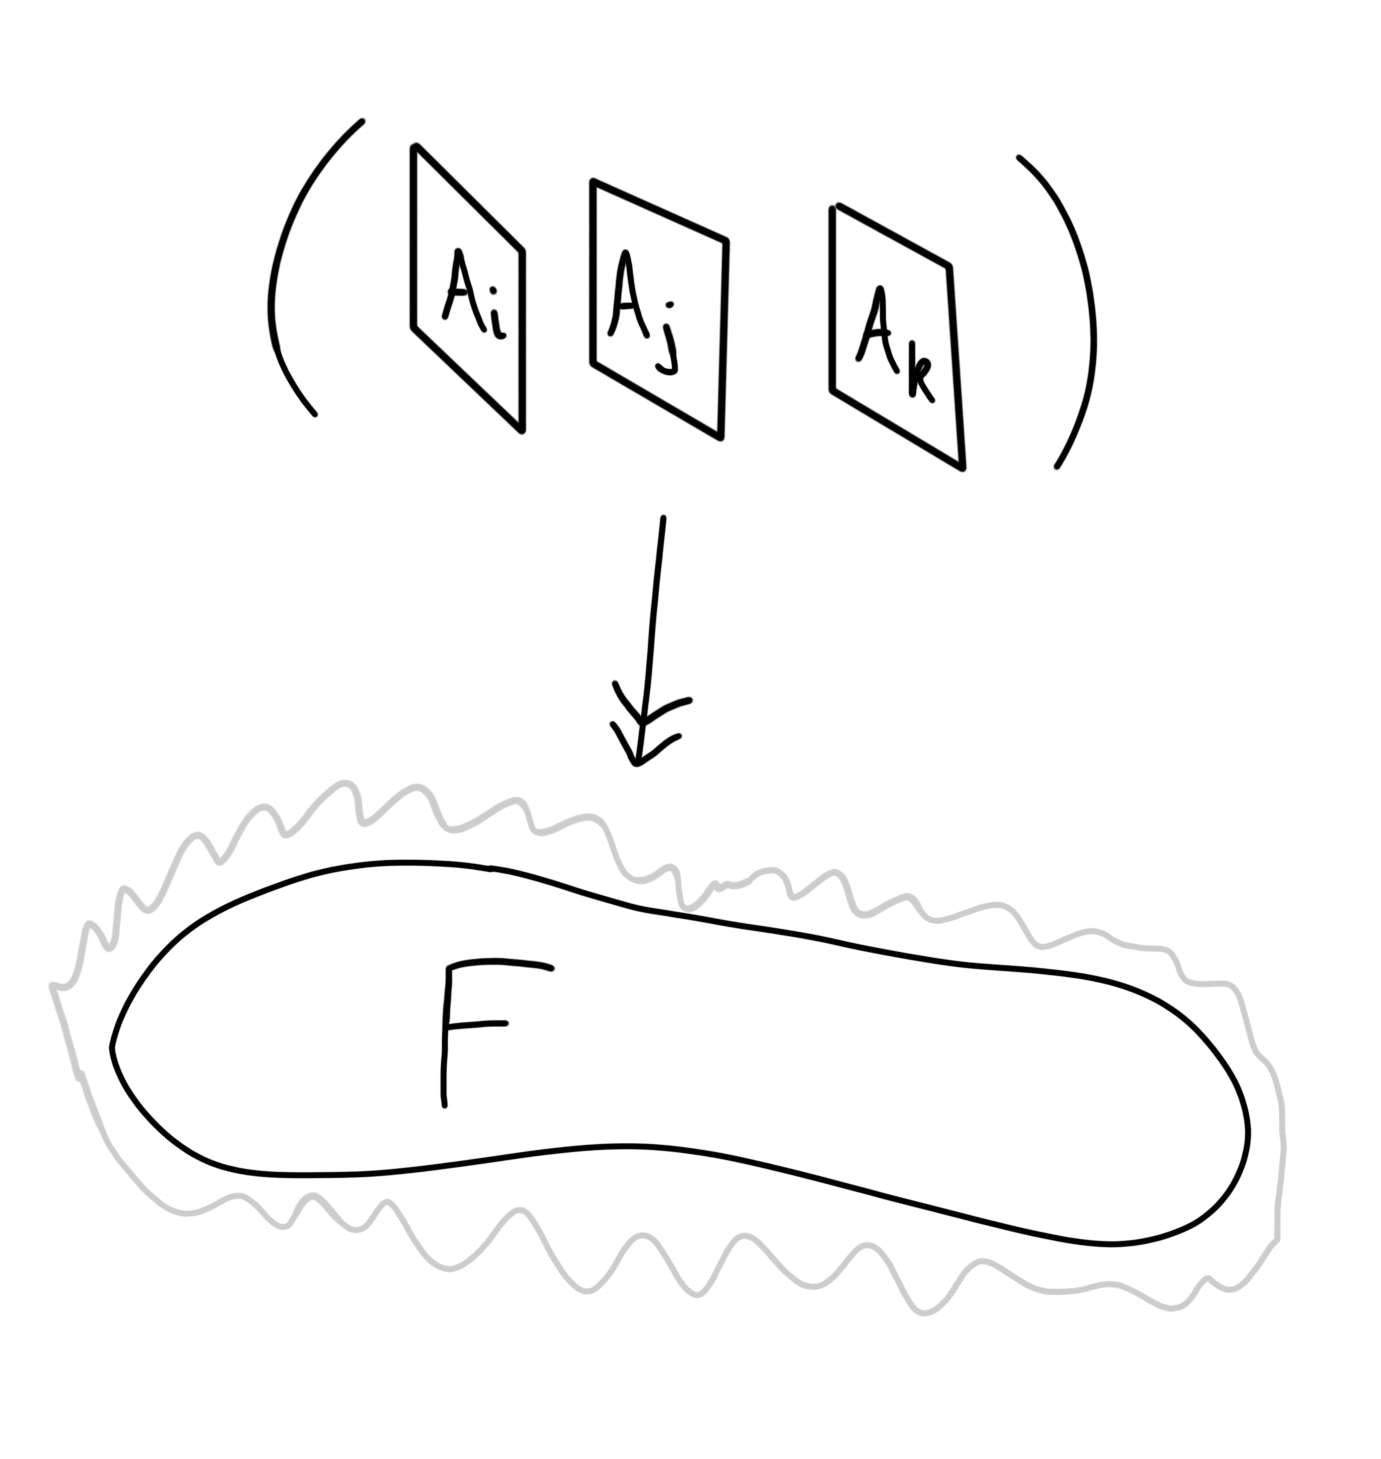
\includegraphics[width=\textwidth]{images/example-diagram.png}}
        %     \end{minipage}
        %     \hspace{0.02\textwidth}
        %     \begin{minipage}[t]{0.48\textwidth}
        %         \vspace{0pt}
        %         \caption{The diagram corresponding to the statement `if a sheaf $F$ has an affine Zariski cover $\{A_i\}$ then it is a scheme' -- the lighter grey corresponds to the hypotheses on $F$ -- in an attempt to retain simplicity here we don't use any notation to show if a map is Zariski open}\label{fg:example-diagram}
        %     \end{minipage}
        % \end{figure}

        % \begin{figure}[p]
        %     \centering
        %     \begin{minipage}[t]{0.73\textwidth}
        %         \vspace{0pt}
        %         \frame{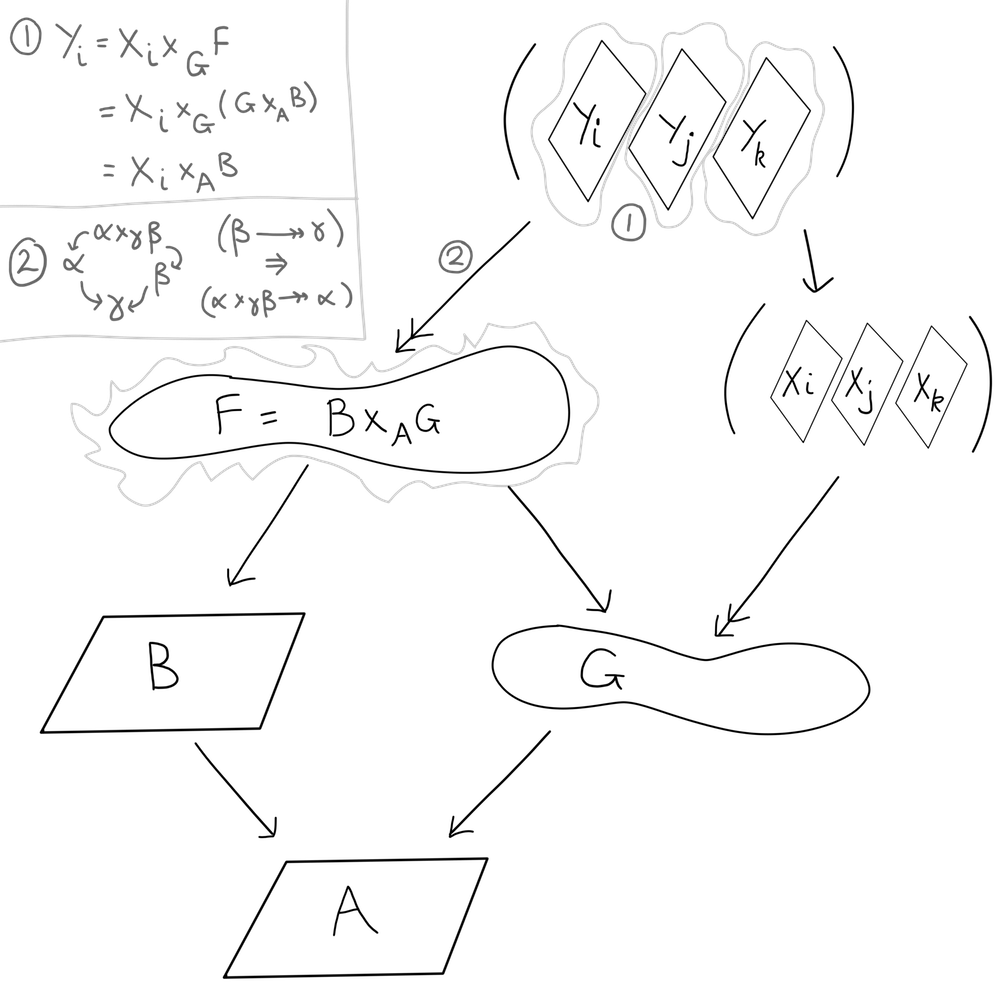
\includegraphics[width=\textwidth]{images/recollement-affine-i.png}}
        %         \caption{\Cref{le:recollement-and-affine}(i)}\label{fg:recollement-affine-i}
        %     \end{minipage}
        %     \hfill
        %     \begin{minipage}[t]{0.23\textwidth}
        %         \vspace{0pt}
        %         {\footnotesize The proof of \numberincircle{1} uses \emph{pasting of pullbacks} and tells us that the $Y_i$ are affine schemes, because \mbox{$\spec\alpha\times_{\spec\beta}\spec\gamma$} \mbox{$\cong\spec(\alpha\coprod_\beta\gamma)$};}
        %         % \begin{align*}
        %         %     &\spec\alpha\times_{\spec\beta}\spec\gamma\\
        %         %     &\cong\spec(\alpha\coprod_\beta\gamma);
        %         % \end{align*}
        %         {\footnotesize the proof of \numberincircle{2} simply says that the pullback of an epimorphism is also an epimorphism}
        %     \end{minipage}
        % \end{figure}

        % \begin{figure}[p]
        %     \centering
        %     \begin{minipage}[t]{0.73\textwidth}
        %         \vspace{0pt}
        %         \frame{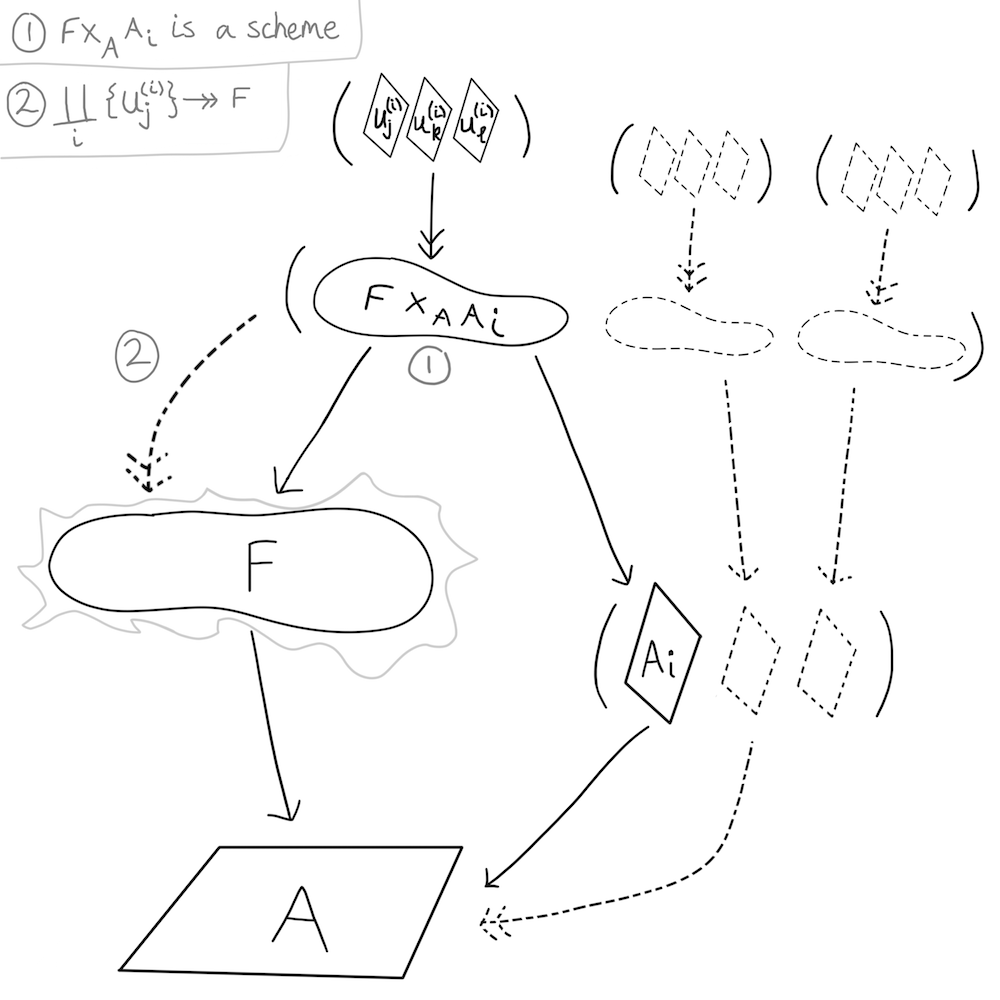
\includegraphics[width=\textwidth]{images/recollement-affine-ii.png}}
        %         \caption{\Cref{le:recollement-and-affine}(ii)}\label{fg:recollement-affine-ii}
        %     \end{minipage}
        %     \hfill
        %     \begin{minipage}[t]{0.23\textwidth}
        %         \vspace{0pt}
        %         {\footnotesize For \numberincircle{1} the previous part of the lemma tells us that \mbox{$F\times_A A_i$} is a scheme; \numberincircle{2} says that if we take affine covers for all of the \mbox{$F\times_A A_i$} then together they cover~$F$}
        %     \end{minipage}
        % \end{figure}

        \begin{figure}[h!]
            \centering
            \frame{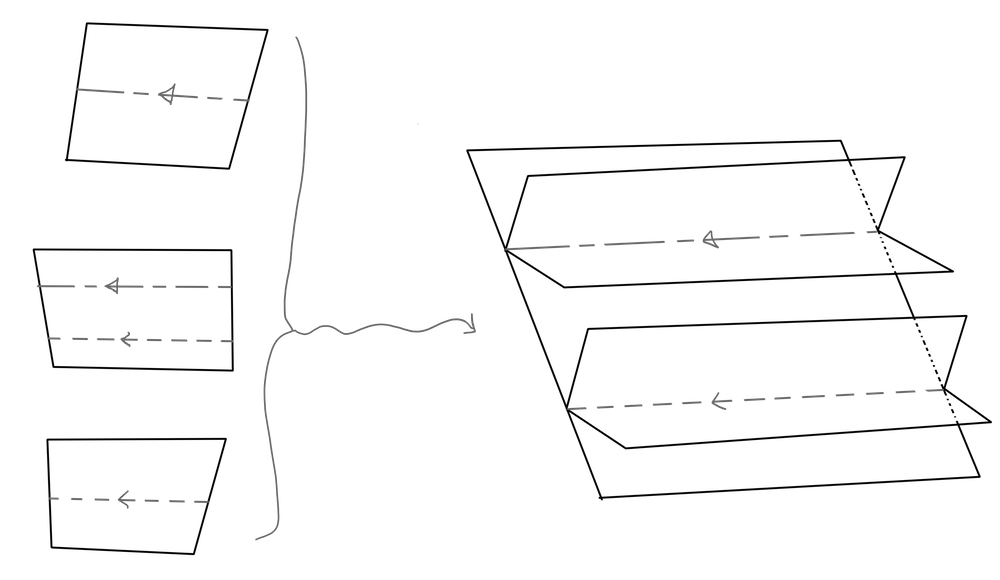
\includegraphics[width=.6\textwidth]{images/gluing.png}}
            \caption{Rephrasing \cref{le:actual-gluing}(ii) in familiar `gluing' terms -- if we take some affine schemes with Zariski-open affine subschemes and glue along these subschemes in a `sufficiently nice' way, then we end up with a scheme -- further, every scheme is obtained in exactly this way -- \emph{schemes are affine schemes glued together}}\label{fg:gluing}
        \end{figure}

    % subsubsection properties_of_schemes (end)





    \subsubsection{Another view} % (fold)
    \label{ssub:another_view}

        Here we briefly discuss how the functor of points approach that we have been using (\cref{sub:background_knowledge}) coincides with the classical ringed space approach.
        % As mentioned in \cref{sub:background_knowledge}, we have been using the functor of points approach, but we now discuss how we could have instead used the ringed space approach, and how these two notions coincide.
        What follows is a sketch of the story -- in particular we make claims without stating proofs -- and we refer the reader to the end (the last four paragraphs) of \cite[\S2.4, p.24]{Toen:2005wxa} as well as \cite[\S IX.1--3]{MacLane:1992uz} for the details.

        \bigskip

        Given some topological space $T$ we can view the category $\Op{T}$ as a lattice, with partial order given by inclusion.
        Generally, define a \emph{frame} to be any lattice $X$ that behaves suitably like $\Op{T}$: having arbitrary joins and finite meets, and meets distributing over arbitrary joins.
        The morphisms between frames are maps of partially-ordered sets preserving arbitrary joins and finite meets.
        This defines a category $\Fra$ of frames.
        We define the category of \emph{locales}\footnote{
            Translation note: locales are called \emph{lieux} in French.
        } as $\Loc=\op{\Fra}$, and for $f\colon X\to Y$ in $\Loc$ we write $f^{-1}\colon\mathcal{O}(Y)\to\mathcal{O}(X)$ to be the corresponding morphism of objects in $\Fra$.

        Next, given a locale $X$ we can define \emph{points of $X$} as locale morphisms $1\to X$, where $1\in\Loc$ is the terminal locale.
        We say that a locale \emph{has enough points} if elements of the lattice can be distinguished by a single point\footnote{
            \Cite[\S IX.2]{MacLane:1992uz} provides a nice way of thinking of this in terms of frames.
        }.
        That is, for any distinct $U,V\in\mathcal{O}(X)$, there exists $p\colon\singleton\to X$ such that $p^{-1}(U)\neq p^{-1}(V)$.
        It can be shown\footnote{
            \cite[Corollary~4,~\S IX.3]{MacLane:1992uz}
        } that if a locale $X$ has enough points then there exists some topological space $|X|$ such that $\mathcal{O}(X)\cong\Op{|X|}$.

        Finally, given $X\in\Sch(\ccat)$, we define $\Zar{X}$ as the full subcategory of $\Shv(\aff{\ccat})/X$ consisting of $u\colon Y\to X$ such that $Y$ is a scheme and $u$ is an open Zariski immersion.
        It turns out that $\Zar{X}$ is a locale, and it has an induced topology coming from the canonical topology on $\Shv(\aff{\ccat})$.
        If we define $\AffZar{X}$ to be the full subcategory of $\Zar{X}$ consisting of $Y\to X$ with $Y$ an affine scheme, and endow this with the same restricted topology, then we have the equivalence of categories
        \begin{equation*}
            \Shv(\Zar{X})\equiv\Shv(\AffZar{X}),
        \end{equation*}
        so we write $\Shv(X_\text{Zar})$ to mean either (under this identification).
        The topology on $\Zar{X}$ is generated by a quasi-compact pretopology (i.e. finite covering families), namely $\AffZar{X}$.
        This means that $\Zar{X}$ has enough points\footnote{
            More generally, \emph{Deligne's theorem} (\cite[Corollary~3,~\S IX.11]{MacLane:1992uz}) tells us that any \emph{coherent topos} has enough points.
        }, and so, by the above, $\Zar{X}\equiv\Op{|X|}$ for some topological space $|X|$.
        This induces the equivalence
        \begin{equation*}
            \Shv(X_\text{Zar})\equiv\Shv(|X|).
        \end{equation*}

        \bigskip

        Now let $Y=(\spec A\to X)\in\AffZar{X}$.
        We can associate to $Y$ the object $A\in\comm{\ccat}$; letting $Y$ vary over $\AffZar{X}$ induces a functor
        \begin{align*}
            \mathcal{O}_X\colon\op{\AffZar{X}}&\to\comm{\ccat}\\
            (X\to\spec A)&\mapsto A.
        \end{align*}
        Then $\mathcal{O}_X$ is a sheaf\footnote{
            \Cref{le:essential-image-is-fpqc}
        }, and the pair $(|X|,\mathcal{O}_X)$ acts as in a $\ccat$-ringed space approach.
        Replacing $\ccat$ with $\Ab$ we recover the classical ringed space approach.

    % subsubsection another_view (end)


        \begin{figure}[h!]
            \centering
            \frame{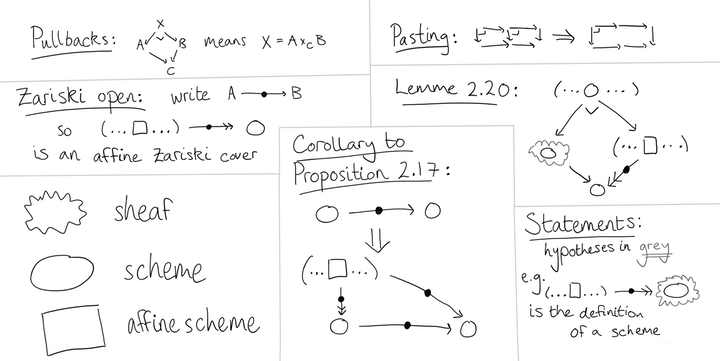
\includegraphics[width=\textwidth]{images/diagram-key-new.png}}
            \caption{The motivation of the notation is the naive motto `straight lines are simpler than curved ones': affine schemes are our building blocks, schemes are slightly more complicated, and sheaves are the least well behaved of all -- \emph{the choice of graphical notation is not meant to be read into too deeply}}
            \label{fg:diagram-key}
        \end{figure}

        \begin{figure}[h!]
            \centering
            \frame{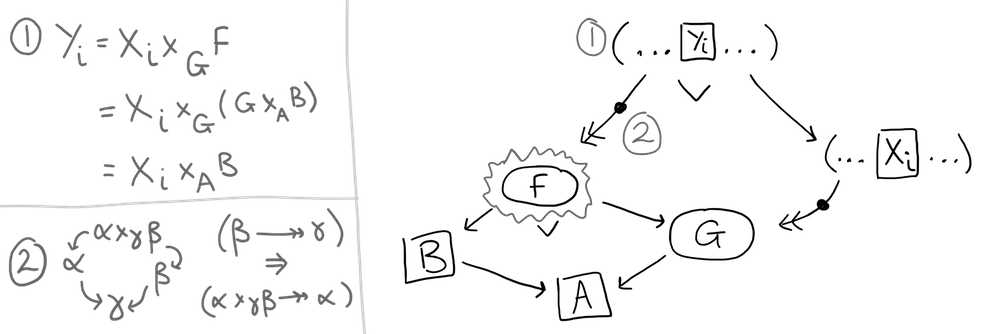
\includegraphics[width=\textwidth]{images/recollement-affine-i-new.png}}
            \caption{\cref{le:recollement-and-affine}(i) -- the proof of \numberincircle{1} uses \emph{pasting of pullbacks} and tells us that the $Y_i$ are affine schemes, because $\spec\alpha\times_{\spec\beta}\spec\gamma\cong\spec(\alpha\coprod_\beta\gamma)$; the proof of \numberincircle{2} simply says that the pullback of an epimorphism is also an epimorphism}\label{fg:recollement-affine-i}
        \end{figure}


        \begin{figure}[h!]
            \centering
            \begin{minipage}[t]{0.73\textwidth}
                \vspace{0pt}
                \frame{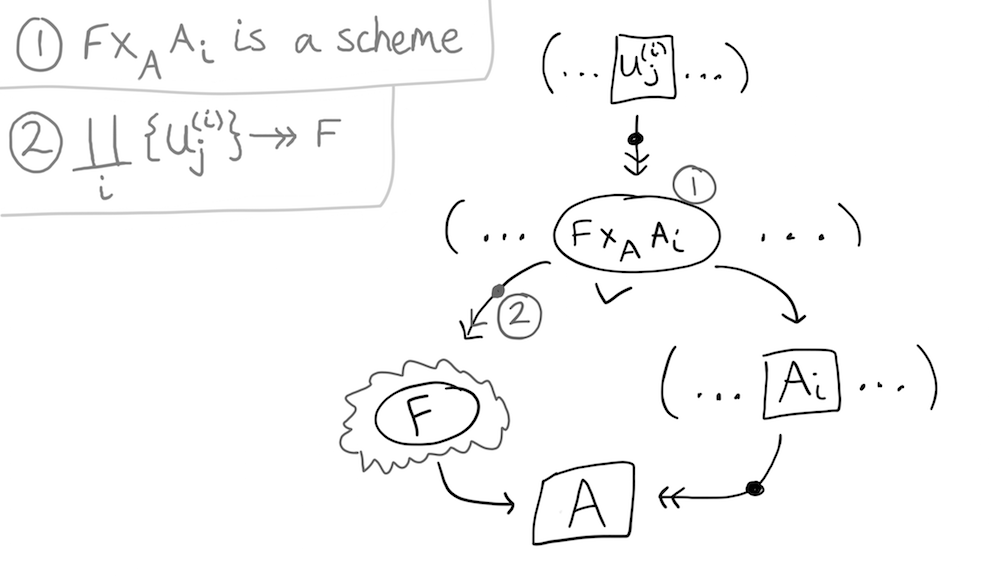
\includegraphics[width=\textwidth]{images/recollement-affine-ii-new.png}}
                \caption{\Cref{le:recollement-and-affine}(ii) -- a special case of \cite[Lemme~2.20,~\S2.4]{Toen:2005wxa}}\label{fg:recollement-affine-ii}
            \end{minipage}
            \hfill
            \begin{minipage}[t]{0.23\textwidth}
                \vspace{0pt}
                {\footnotesize For \numberincircle{1} the previous part of the lemma tells us that \mbox{$F\times_A A_i$} is a scheme; \numberincircle{2} says that if we take affine covers for all of the \mbox{$F\times_A A_i$} then together they cover~$F$}
            \end{minipage}
        \end{figure}

        \begin{figure}[h!]
            \centering
            \begin{minipage}[t]{0.73\textwidth}
                \vspace{0pt}
                \frame{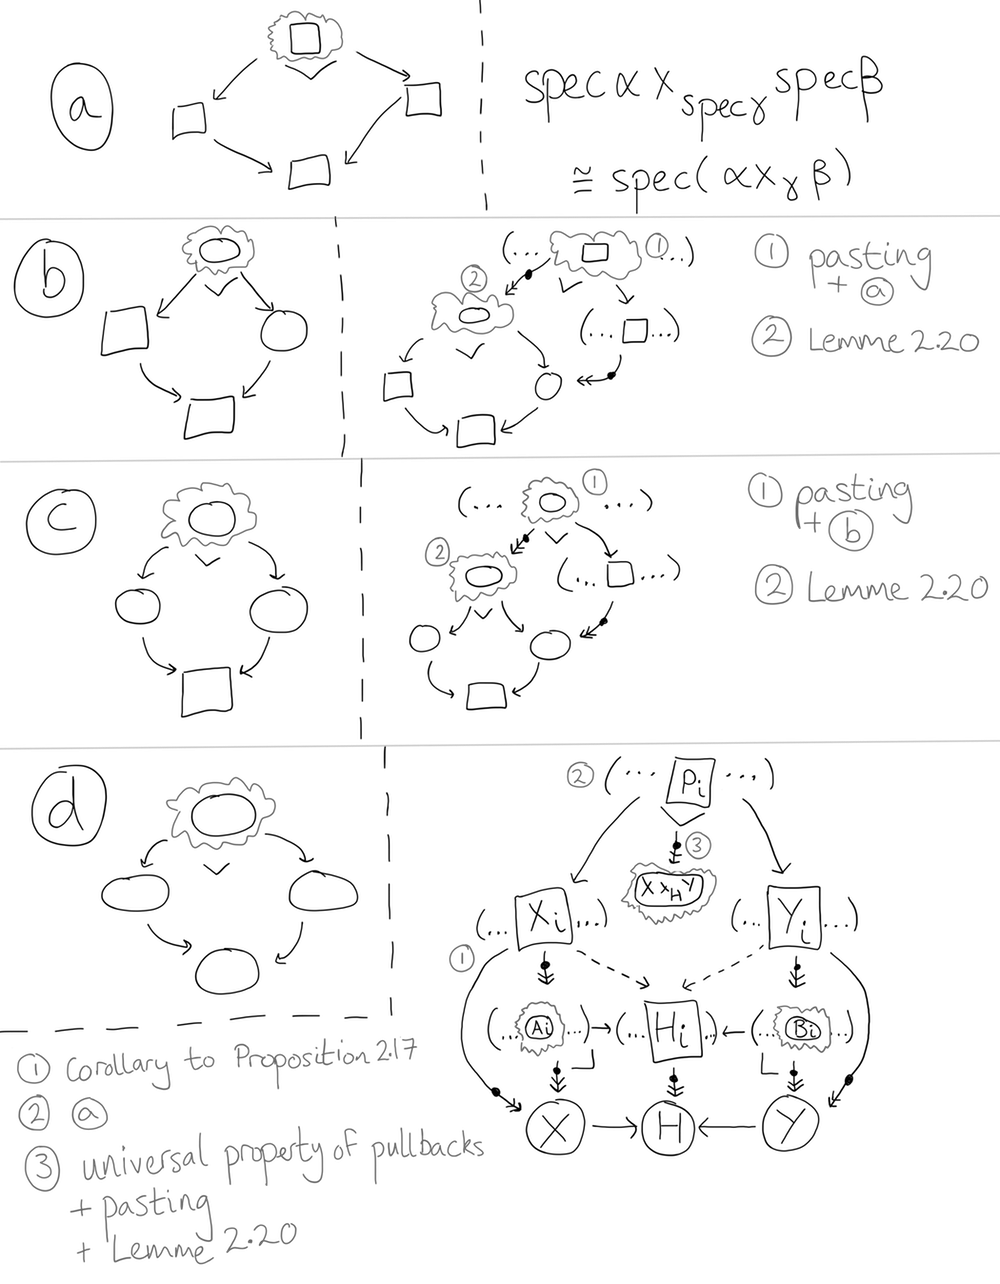
\includegraphics[width=\textwidth]{images/stability.png}}
                \caption{\Cref{le:actual-gluing}(i) -- the statement concerning pullbacks}\label{fg:stability}
            \end{minipage}
            \hfill
            \begin{minipage}[t]{0.23\textwidth}
                \vspace{0pt}
                {\footnotesize We build up to this proof in successive steps, from \numberincircle{a} to \numberincircle{d} -- the statements are on the left and the proofs on the right}
            \end{minipage}
        \end{figure}



% subsection schemes (end)



% !TEX root = ../../../under-spec-z.tex

\subsection{Changes of base} % (fold)
\label{sub:changes_of_bases}

    % \emph{Throughout this section $(\ccat,\otimes,1_\ccat)$ and $(\dcat,\odot,1_\dcat)$ are both cosmoses.}

    The aim of this section is to provide some technical machinery that we will use in \cref{sec:three_examples_of_relative_geometry}, so we only state the main result of \cite[\S2.5]{Toen:2005wxa} and refer the reader back to there for more details.

    % \bigskip

    % Suppose we have some strong\footnote{
    %     \cite{Toen:2005wxa} uses the name \emph{monoidal functor} (as do many other sources) to refer to what is sometimes called a \emph{strong monoidal functor}.
    %     The choice of nomenclature is only important insofar as consistency; we decide to use `strong'.
    % } symmetric monoidal functor\footnote{
    %     That is, a functor that respects the symmetric monoidal structure of both $\ccat$ and $\dcat$.
    %     To be slightly more precise, the functor comes with an isomorphism $f(X)\odot f(Y)\congto f(X\otimes Y)$, natural in $X$ and $Y$, which respects the symmetry of $\otimes$ and $\odot$, and an isomorphism $1_\dcat\congto f(1_\ccat)$ satisfying certain coherence conditions.
    % } \mbox{$f\colon\ccat\to\dcat$} that has a right adjoint $g\colon\dcat\to\ccat$.
    % This right adjoint is not necessarily a strong monoidal functor, but it is a \emph{lax monoidal functor}\footnote{
    %     That is, we do have morphisms $g(X)\otimes g(Y)\to g(X\odot Y)$ and $1_\ccat\to g(1_\dcat)$ respecting coherence conditions and the symmetry of $\otimes$ and $\odot$, but they are not necessarily isomorphisms.
    % }, which turns out to be enough for $g$ to induce a functor on the categories of commutative monoids and on the category of modules.

    % By its symmetric monoidality, the functor $f\colon\ccat\to\dcat$ induces a functor $f\colon\aff{\ccat}\to\aff{\dcat}$.
    % This in turn induces a functor $f_!^\sim\colon\Shv(\aff{\ccat}\to\Shv(\aff{\dcat})$, given by precomposition by $g$ (and the use of \emph{sheafification}\footnote{
    %     Similar to classical algebraic geometry, the inclusion functor $\iota\colon\Shv(\aff{\ccat})\to\PShv(\aff{\ccat})$ admits a left adjoint $a\colon\PShv(\aff{\ccat})\to\Shv(\aff{\ccat})$ which we call the \emph{sheafification functor}.
    %     For (vastly many) more details, see \cite[\S III.5,~Theorem~1]{MacLane:1992uz}.
    % }).

    \begin{theorem}[\mbox{}{(Corollaire~2.22,~\S2.5,~p.27)}]\label{co:that-base-change-lemma-that-is-important}
        Let $(\ccat,\otimes,1_\ccat)$ and $(\dcat,\odot,1_\dcat)$ be cosmoses, and $f\colon\ccat\to\dcat$ be a strong symmetric monoidal functor\footnote{
            That is, a functor that respects the symmetric monoidal structure of both $\ccat$ and $\dcat$.
            To be slightly more precise, the functor comes with an isomorphism $f(X)\odot f(Y)\congto f(X\otimes Y)$, natural in $X$ and $Y$, which respects the symmetry of $\otimes$ and $\odot$, and an isomorphism \mbox{$1_\dcat\congto f(1_\ccat)$} satisfying certain coherence conditions.
            \cite{Toen:2005wxa} and many others use the name \emph{monoidal functor} to refer to what we (and some others) call a \emph{strong monoidal functor}.
            The choice of nomenclature is only important insofar as consistency; we agree to use `strong'.
        } with left adjoint $g\colon\dcat\to\ccat$.
        Define
        % \begin{align*}
        %     f_!\colon\PShv(\aff{\ccat})&\to\PShv(\aff{\dcat})\\
        %     F&\mapsto(F\circ g)
        % \end{align*}
        % and
        \begin{align*}
            f_!^\sim\colon\Shv(\aff{\ccat})&\to\Shv(\aff{\dcat})\\
            F&\mapsto(a\circ F\circ g)
        \end{align*}
        where $a$ is the \emph{sheafification}\footnote{
            Similar to classical algebraic geometry: the inclusion functor $\iota\colon\Shv(\aff{\ccat})\to\PShv(\aff{\ccat})$ admits a left adjoint $a\colon\PShv(\aff{\ccat})\to\Shv(\aff{\ccat})$ which we call the \emph{sheafification functor}.
            For (vastly many) more details, see \cite[\S III.5,~Theorem~1]{MacLane:1992uz}.
        } functor.
        Suppose that $g\colon\dcat\to\ccat$ is conservative and commutes with filtered colimits, and that, for every flat morphism $A\to B$ in $\comm{\ccat}$ and every $N\in \modc{f(A)}$, the natural morphism
        \begin{equation*}
            g(N)\otimes_A B\to g(N\odot_{f(A)}f(B))
        \end{equation*}
        is an isomorphism in $\modc{B}$.
        Then
        \begin{enumerate}[(i)]
            \item $f\colon\aff{\ccat}\to\aff{\dcat}$ is continuous in the Zariski topology;
            \item the functor $f_!^\sim\colon\Shv(\aff{\ccat})\to\Shv(\aff{\dcat})$ preserves the subcategories of schemes, and induces a functor (called the \emph{change of base functor})
                \begin{align*}
                    \Sch(\ccat)&\to\Sch(\dcat)\\
                    X&\mapsto X\otimes\dcat := f_!^\sim(X);
                \end{align*}
            \item we have an isomorphism
                \begin{equation*}
                    f_!^\sim(X)\cong f(X)
                \end{equation*}
                for every $X\in\ASch(\ccat)$.\qedhere
        \end{enumerate}
    \end{theorem}

    % \begin{proof}
    %     See \cite{Toen:2005wxa}.
    % \end{proof}

    \begin{note}[Notation]
        Say $(\mathcal{T},\otimes,1)$ is a cosmos and $A,B\in\comm{\mathcal{T}}$.
        Then, with $\ccat=\modc{A}$ and $\dcat=\modc{B}$, we write
        \begin{equation*}
            F_!^\sim(\blank)=(\blank\otimes_A B)\colon\Sch(\modc{A})\to\Sch(\modc{B}),
        \end{equation*}
        extending the definition of $(\blank\otimes_A B)$ from \cref{ssub:commutative_algebras}.
    \end{note}

    % The functor $F$ induces a functor $\comm{\ccat}\to\comm{\ccat}$, and thus $\aff{\ccat}\to\aff{\dcat}$, and this latter functor has a \emph{left}\footnote{
    %     Since $\aff{\ccat}$ is defined as the opposite category $\comm{\ccat}$, the handedness of the adjunction swaps when we descend to the induced functors.
    % } adjoint, induced by $G$.
    % That is, keeping the same notation for the induced functors as the original functors,
    % \begin{equation*}
    %     (G\colon\aff{\dcat}\to\aff{\ccat}) \dashv (F\colon\aff{\ccat}\to\aff{\dcat}).
    % \end{equation*}

    % Now, the functor $G\colon\aff{\dcat}\to\aff{\ccat}$ induces a functor on presheaf categories
    % \begin{equation*}
    %     G^*\colon\PShv(\aff{\ccat})\to\PShv(\aff{\dcat})
    % \end{equation*}
    % given, on objects, by precomposition:
    % \begin{equation*}
    %     G^*\colon X\mapsto (X\circ G),
    % \end{equation*}
    % and similarly for $F^*$.
    % We claim that there exists a left adjoint $G_!\dashv G^*$, and that it is given by $G_!=F^*$.
    % We do not prove this fact here, but it can be done in various ways\footnote{
    %     In our particularly nice situation (assuming smallness of categories, and using the fact that $\Set$ is, in particular, cocomplete) we can construct a left-adjoint $G_!$ for $G^*$ using the \emph{left Kan extension functor}.
    %     In fact, since $\Set$ is also complete, we also have a right adjoint $G^*\dashv G_*$, which turns out to be given by $G_*=F^*$.
    %     Full details can be found in \cite[\S X.3]{Lane:1998fe}.
    % }.

    % In fact, the adjuction $(F_!\dashv F^*)$ induces an adjuction $(F_!^\sim \dashv F^*)$ on the category of sheaves, where we use the \emph{sheafification\footnote{
    %     Similar to classical algebraic geometry, the inclusion functor $\iota\colon\Shv(\aff{\ccat})\to\PShv(\aff{\ccat})$ admits a left adjoint $a\colon\PShv(\aff{\ccat})\to\Shv(\aff{\ccat})$ which we call the \emph{sheafification functor}.
    %     For (vastly many) more details, see \cite[\S III.5,~Theorem~1]{MacLane:1992uz}.
    % } functor $a$} to define
    % \begin{equation*}
    %     F_!^\sim=(a\circ F_!)\colon\Shv(\aff{\ccat})\to\Shv(\aff{\dcat}).
    % \end{equation*}
    % Since $F$ has a right adjoint, and thus commutes with colimits, $F_!^\sim$ commutes in particular with finite limits.
    % An adjuction $(f\dashv g)$ between sites\footnote{
    %     It should really be an adjuction between \emph{toposes}, though we don't have time to discuss this notion properly.
    % } is said to be a \emph{geometric morphism} if $f$ commutes with finite limits, and we have just shown that $(F_!^\sim \dashv F^*)$ is such an adjuction.
    
    % \begin{definition}[Continuous in a topology]\label{df:continuous-in-topology}
    %     A functor $F\colon\aff{\ccat}\to\aff{\dcat}$ is said to be \emph{continuous in the Zariski} (resp. \emph{fpqc}) \emph{topology} if the induced functor
    %     \begin{equation*}
    %         F^*\colon\PShv(\aff{\dcat})\to\PShv(\aff{\ccat})
    %     \end{equation*}
    %     (as defined above) preserves the subcategory of Zariski (resp. fpqc) sheaves.
    % \end{definition}

    % Note that this definition is different from the definition of a continuous functor in the sense of preserving small limits.
    % Because of this we will always ensure to talk of a functor being continuous \emph{in a topology} if we mean continuous in the sense of \cref{df:continuous-in-topology}.

    % \begin{lemma}[\mbox{}{Proposition~2.21,~\S2.5,~p.26}]
    %     Using the above notation,
    %     \begin{enumerate}[(i)]
    %         \item $F\colon\aff{\ccat}\to\aff{\dcat}$ preserves monomorphisms and finite limits;
    %         \item if $F\colon\aff{\ccat}\to\aff{\dcat}$ is continuous in the fpqc topology and $G\colon\dcat\to\ccat$ commutes with filtered colimits, then $F\colon\aff{\ccat}\to\aff{\dcat}$ is also continuous in the Zariski topology.\qedhere
    %     \end{enumerate}
    % \end{lemma}

    % \begin{proof}
    %     This is largely just unpacking definitions.
    %     See \cite{Toen:2005wxa}.
    % \end{proof}

    % \begin{corollary}[\mbox{}{(Corollaire~2.22,~\S2.5,~p.27)}]\label{co:that-base-change-lemma-that-is-important}
    %     Using the above notation, suppose that the functor $G\colon\dcat\to\ccat$ is conservative and commutes with filtered colimits.
    %     Suppose further that, for every flat morphism $A\to B$ in $\comm{\ccat}$ and every $N\in \modc{F(A)}$, the natural morphism
    %     \begin{equation*}
    %         G(N)\otimes_A B\to G(N\odot_{F(A)}F(B))
    %     \end{equation*}
    %     is an isomorphism in $\modc{B}$.
    %     Then
    %     \begin{enumerate}[(i)]
    %         \item $F\colon\aff{\ccat}\to\aff{\dcat}$ is continuous in the Zariski topology;
    %         \item the functor $F_!^\sim\colon\Shv(\aff{\ccat})\to\Shv(\aff{\dcat})$ preserves the subcategories of schemes, and induces a functor
    %             \begin{align*}
    %                 \Sch(\ccat)&\to\Sch(\dcat)\\
    %                 X&\mapsto X\otimes\dcat := F_!^\sim(X);
    %             \end{align*}
    %         \item we have an isomorphism
    %             \begin{equation*}
    %                 F_!^\sim(X)\cong F(X)
    %             \end{equation*}
    %             for every $X\in\ASch(\ccat)$.\qedhere
    %     \end{enumerate}
    % \end{corollary}

    % \begin{proof}
    %     See \cite{Toen:2005wxa}.
    % \end{proof}

    % \begin{note}[Notation]
    %     Say $(\mathcal{T},\otimes,1)$ is a cosmos and $A,B\in\comm{\mathcal{T}}$.
    %     Then, with $\ccat=\modc{A}$ and $\dcat=\modc{B}$, we write
    %     \begin{equation*}
    %         F_!^\sim(\blank)=(\blank\otimes_A B)\colon\Sch(\modc{A})\to\Sch(\modc{B}),
    %     \end{equation*}
    %     extending the definition of $(\blank\otimes_A B)$ from \cref{ssub:commutative_algebras}.
    % \end{note}

    
    As we would (very much) hope, the change of base functor is functorial: it doesn't matter in which order we change base and sheafify.
    In particular, if $X=\spec A\in\aff{\ccat}$ for some $A\in\comm{\ccat}$ then \cref{co:that-base-change-lemma-that-is-important}~(iii) tells us\footnote{
        \cite[\S2.5,~\P-1]{Toen:2005wxa}
    } that
    \begin{equation*}
        f_!^\sim(\spec A)\cong\spec f(A).
    \end{equation*}
    Thus, using the Hom-set isomorphism from the adjunction $(f\dashv g)$,
    \begin{align*}
        f_!^\sim(\spec A)\colon\comm{\dcat}&\to\Set\\
        B&\mapsto\Hom(f(A),B)\cong\Hom(A,g(B)).
    \end{align*}
    We think of $\spec f(A)$ as\footnote{
        Again, recall \cref{df:affine-schemes-general}.
    }
    \begin{align*}
        \spec f(A) \quad\mlq=\mrq\quad &\Hom_{\aff{\dcat}}(\blank,\spec f(A))\\
        =&\Hom_{\comm{\dcat}}(f(A),\blank).
    \end{align*}
    So, remembering \cref{ssub:motivating_example}, $f_!^\sim(\spec A)$ gives the \emph{functor of points of $A$}.

    % As we would (very much) hope, the change of base functor is functorial: spelling out \cref{co:that-base-change-lemma-that-is-important}~(iii) below tells us that it doesn't matter in which order we change base and sheafify.

    % \begin{translation}{2.5}{-1}
    %     For a commutative monoid $A\in\comm{\ccat}$ we have a natural isomorphism
    %     \begin{equation*}
    %         F_!^\sim(\spec A)\cong\spec F(A).
    %     \end{equation*}
    %     Indeed, by definition the functor $F_!^\sim$ is the composition of $F_!$ (defined on presheaves) and $a$ (the sheafification functor).
    %     It is easy to see that $F_!(\spec A)\cong\spec F(A)$ as \emph{presheaves}.
    %     Since presheaves that are representable by affine schemes are sheaves, we see that $F_!^\sim(\spec A)\cong\spec F(A)$.
    %     This tells us that
    %     \begin{align*}
    %         F_!^\sim(\spec A)\colon\comm{\dcat}&\to\Set\\
    %         B&\mapsto\Hom_{\comm{\ccat}}(A,G(B)).
    %     \end{align*}
    %     for all $\spec A\in\aff{\ccat}$.
    % \end{translation}

    % TJH what does this mean?
    % TJH recall functor of points ($\Hom(A,\blank)$) and use Yoneda \emph{lemma}
    % ...
    % \begin{align*}
    %     &F_!^\sim(\spec A)(\blank)\\
    %     \cong &\Hom_{\comm{\dcat}}(F(A),\blank)\\
    %     \cong &\Hom_{\PShv(\aff{\dcat})}(\spec \blank,\spec F(A))\in\PShv(\aff{\dcat})
    % \end{align*}
    % \textbf{\emph{...so what?}}
    % the second one doesn't need Yoneda, but looks like the functor of points approach for $F(A)$?

% subsection changes_of_bases (end)


% section relative_algebraic_geometry (end)

    \clearpage
    % \input{content/sections/three-examples/three-examples.tex}
    % !TEX root = ../../under-spec-z.tex

\section{Three examples of relative geometry} % (fold)
\label{sec:three_examples_of_relative_geometry}

    \emph{We now present our first three examples of categories of relative schemes.} (\S3~\P1)

    \begin{note}
        As stated in \cref{ssub:conventions}, we adopt the convention that $0\in\nn$.
    \end{note}

    \subsection{Under $\spec\zz$} % (fold)
    \label{sub:under_}

        Instead of just restating the results of \cite[\S3.1--3.3,~4]{Toen:2005wxa} we try here to provide some motivation for these choices of examples.

        \bigskip

        We know that $\zz$ is the initial object in the category $\CRing$ of commutative rings; we said in \cref{sub:overview} that we would have to leave $\CRing$ in order to find schemes over bases that lie \emph{under} $\spec\zz$.
        If we remove all algebraic structure from $\CRing$ we end up with the category $\Set$ of sets, and we might worry that we have discarded too much structure to be able to define schemes any more.
        But $(\Set,\times,\singleton)$, where $\times$ is the cartesian product and $\singleton$ is a singleton, \emph{is} a cosmos\footnote{
            It is arguably the most tautological example of a cosmos.
        }, and so we can define schemes over $\Set$.
        Since $\Set$ is the prototype of a concrete category we can't really go down any further without becoming too far removed from our usual concept of algebraic structures.
        So we look at what (commutative associative and unital) structures we can find in between $\Set$ and $\CRing$.

        % We can endow a set with some commutative associative binary operation, which we might as well call addition, and pick an object to be the additive identity.
        % This results in a \emph{commutative monoid}.
        % All of the language that we have built so far heavily depends on the objects we study having \emph{commutative} and \emph{associative} operations, as well as an \emph{identity}.
        % So we have actually passed over a few less-strict structures -- \emph{semigroups} (where we don't require an identity) and \emph{magmas} (where we don't require associativity) -- but our tools are not general enough to deal with them.

        % Next we could go one of two ways: introducing additive inverses to our commutative monoid, thus making it an \emph{abelian group}; introducing some commutative multiplication with identity, thus making it a \emph{commutative semi\-ring}.
        % Either way, the only thing (of interest to us now) sitting above these two structure comes from combining the two, resulting in a \emph{commutative ring} -- this is where we stop, since classical algebraic geometry can deal with things from here on in.

        We can endow a set with some commutative associative binary operation, which we might as well call addition, and pick an object to be the additive identity -- this results in a \emph{commutative monoid}.
        Then we could go one of two ways: introducing additive inverses to our commutative monoid, making it an \emph{abelian group}; or introducing some commutative multiplication with identity, making it a \emph{commutative semi\-ring}.
        Either way, the only thing (of interest to us now) sitting above these two structure comes from combining the two, resulting in a \emph{commutative ring} -- this is where we stop, since classical algebraic geometry can deal with things from here.

        \begin{note}
            A very important thing to be aware of (that notation doesn't make entirely clear) is that when we speak about $\modc{A}$ for $A\in\comm{\ccat}$, \emph{this category depends on $\ccat$}.
            For example, if we take $\zz\in\comm{\Ab}=\CRing$ then $\modc{\zz}$ is the category of abelian groups, but if we consider \mbox{$\zz\in\comm{\Set}=\CMon$} then $\modc{\zz}$ is the category of \emph{monoid actions}, or \emph{$\zz$-actions} (sometimes confusingly written $\zz\hbox{-}\mathsf{Set}$).
            \emph{To avoid confusion in this section, we adopt the following (non-standard) notation:} we write $\modc{A}_\ccat$ to emphasise that \mbox{$A\in\comm{\ccat}$}.
        \end{note}

        Recalling \cref{df:comm-c,df:module-over-monoid}, the following pattern emerges:
        % \footnote{
        %     In fact, there is a much more general statement: when $\smc$ is a cosmos then $1$ is initial in $\comm{\ccat}$, \emph{and} $\modc{1}\equiv\ccat$.
        %     This follows straight from the definitions.
        %     A different way to approach this might be the following: there is a monoidal forgetful functor $\Ab\to\Set$ which lifts to a functor $\modc{A}_\Ab\to\modc{A}_\Set$, and by some abstract nonsense this has an adjoint, so we could hope to lift $X\in\modc{A}_\Set$ to some $X'\in\modc{A}_\Ab$.
        %     But for us, once we know what we are aiming for, it is much easier to start with some algebraic object $A$, and then pick some $\ccat$ with $A\in\comm{\ccat}$ such that $\modc{A}_\ccat$ is exactly what we want it to be.
        % }:
        \begin{equation*}
            \begin{tikzcd}
                & \modc{1}_\ccat & (1,\ccat) & \comm{\modc{1}_\ccat} &\\[-1.8em]
                \,\arrow[rrrr, dash] & & & & \,\\[-1.5em]
                & \Ab & (\zz,\Ab) & \CRing &\\
                & \CMon \arrow[u] & (\nn,\CMon) \arrow[u, "\text{introduce additive inverses}" description] & \CSemiring \arrow[u] &\\
                & \Set \arrow[u] & (\singleton,\Set) \arrow[u, "\text{introduce addition}" description] & \CMon \arrow[u] &
            \end{tikzcd}
        \end{equation*}

        It is true that $\modc{\singleton}_\Set=\Set$, but here lies the subtle issue: when we introduce addition we need our singleton to contain an additive identity \emph{and} an additive generator for $\nn$, but by definition these things must be distinct.
        That is, we want $0,1\in\singleton$ with $0\neq1$.
        Clearly, such a singleton doesn't exist, but in \cite{Tits:1957tq} Jacques Tits introduced the idea of the \emph{field with one element}: $\ff_1$.
        Although it is not a well-defined mathematical object\footnote{
            At least, not within our current definitions of algebraic objects.
        }, it is interesting to put aside such concerns and try to glean as much information from it as possible, especially when it arises in such a natural way as it does here\footnote{
            In fact, studying this $\ff_1$ is one of the main motivations for developing all of this abstract theory -- see \cref{sub:the_riemann_hypothesis}.
        }.

        \bigskip

        By definition, $1$ is initial in $\comm{\ccat}$ and so $\spec1$ is terminal in $\aff{\ccat}$.
        Thus we can think of schemes relative to $\modc{1}_\ccat$ as being schemes \emph{over} $\spec1$.
        It can be shown\footnote{
                These are relatively standard facts -- they can be found, for example, on the $n$Lab.
        } that $(\Ab,\otimes,\zz)$, $(\CMon,\otimes,\nn)$, and $(\Set,\times,\ff_1)$ are all cosmoses.
        In \cite[\S3.1--3.3]{Toen:2005wxa}, the authors work up to defining $\ff_1$-schemes, as well as a base change to $\zz$-schemes:
        \begin{equation}\label{eq:change-of-base-ff1-to-zz}
            (\blank\otimes_{\ff_1}\zz)\colon\schc{\ff_1}\to\schc{\zz}
        \end{equation}
        which acts on affine schemes by
        \begin{equation}\label{eq:ff1-to-zz-affine}
            \begin{alignedat}{3}
                (\blank\otimes_{\ff_1}\zz)\colon\aff{\modc{\ff_1}}&\to\aff{\modc{\nn}}&&\to\aff{\modc{\zz}}\\
                \op{\CMon}&\to\op{\CSemiring}&&\to\op{\CRing}\\
                M&\mapsto\nn[M]&&\mapsto\zz[M].
            \end{alignedat}
        \end{equation}
    
    % subsection under_ (end)







    \subsection{Diagonalisable group schemes} % (fold)
    \label{sub:diagonalisable_group_schemes}

        With \cref{eq:change-of-base-ff1-to-zz} we can try to generalise some constructions of classical schemes to $\schc{\nn}$ and $\schc{\ff_1}$.
        We now look at one such example, straight from \cite[\S4]{Toen:2005wxa}.

        \bigskip

        \emph{\Cite[\S XIV.3,~p.217]{Milne:2012wc} provides a general introduction to diagonalisable group schemes.}
        \emph{The basic idea is to define a functor}
        \begin{align*}
            \dd\colon\Ab&\to\Fun(\CRing,\Grp)\\
            M&\mapsto\Hom_\Grp(M,\blank^\times)
        \end{align*}
        \emph{Then $\dd(M)\colon R\mapsto\Hom_\Grp(M,R^\times)$ can be viewed as an `affine group'.}

        \bigskip

        An abelian group is also a commutative monoid, and $\aff{\modc{\ff_1}}=\op{\CMon}$.
        So for $M\in\Ab$ we can define
        \begin{equation*}
            \dd_{\ff_1}(M) = \spec M\in\schc{\ff_1}.
        \end{equation*}
        Now \cite[Proposition~3.3,~\S XIV.3,~p.217]{Milne:2012wc} tells us two things:
        \begin{enumerate}[(i)]
            \item $\dd(M)\cong\spec\zz[M]$;
            \item if $M$ is finitely generated then $\dd(M)$ is isomorphic to a finite product of copies of $\GG_m$ and $\mu_n$ (for various $n\in\nn$).
        \end{enumerate}
        If we define the affine $\ff_1$-scheme
        \begin{equation*}
            \spec(\ff_{1^n}) = \dd_{\ff_1}(\zz/n\zz)
        \end{equation*}
        then, using the above results and \cref{eq:ff1-to-zz-affine}, we see that
        \begin{enumerate}[(i)]
            \item $\dd_{\ff_1}(M)\otimes_{\ff_1}\zz \cong \dd(M)$;
            \item $\spec(\ff_{1^n})\otimes_{\ff_1}\zz \cong \mu_n \cong \dd(\zz/n\zz)$.
        \end{enumerate}
        So we can generalise $\dd(\blank)$ to $\dd_{\ff_1}(\blank)$ to obtain \emph{diagonalisable group schemes over $\ff_1$} that, after a change of base $\ff_1\to\zz$, agree with our existing notions of diagonalisable group schemes.
        By using a change of base $\ff_1\to\nn$ we can also recover a definition for $\nn$-schemes.

        This idea of $\spec\ff_{1^n}$ plays a major role in \cref{sub:the_riemann_hypothesis}.
    
    % subsection diagonalisable_group_schemes (end)

% section three_examples_of_relative_geometry (end)

    % \clearpage
    % \input{content/sections/some-examples/some-examples.tex}
    \clearpage
    % !TEX root = ../../../under-spec-z.tex

\section{Further applications} % (fold)
\label{sec:further_applications}

    We now look at some applications that are not covered in \cite{Toen:2005wxa}.

% !TEX root = ../../../under-spec-z.tex

\subsection{Day convolution} % (fold)
\label{sub:day_convolution}

    The theory developed in \cite{Toen:2005wxa} is very powerful, but relies on working with a \emph{cosmos} -- we assume, in particular, that our category is bicomplete.
    However, many categories with which we would like to work are \emph{not} bicomplete.
    If this is the case then there are two reasonably natural approaches towards a solution:
    \begin{enumerate}[(i)]
        \item throw away some morphisms -- the fewer the morphisms the `easier' it is for a morphism to be universal in some way;
        \item add in some objects -- `bicomplete' this category in some way.
    \end{enumerate}

    An example of the first approach is when we define the category of Banach spaces to be $\Ban_1$, whose morphisms are weak contractions, instead of the more general $\Ban$, whose morphisms are any bounded linear maps -- $\Ban_1$ is bicomplete\footnote{
        \cite{Yuan:2012vt}
    } whereas $\Ban$ isn't.
    This approach forms the beginning of the study of \emph{categorical Banach space theory}: see e.g. \cite{Anonymous:-VM0nEAk} for explicit descriptions of certain objects and functors (such as the change of base); \cite{Cruttwell:2008wl} for an enriched-category view; and \cite{Castillo:2010vt} for a general survey.

    % \subsubsection{Approach \textrm{(ii)}: $\PShv(\Ban)$} % (fold)
    % \label{ssub:approach_ii}
    
        As for the second approach, it is a standard fact\footnote{
            Since (co)limits are computed pointwise in $\Set$, and $\Set$ is bicomplete.
        } that $\PShv(\dcat)$ is bicomplete for any category $\dcat$, so here we consider $\PShv(\Ban)$.
        But now the issue is giving $\PShv(\Ban)$ a closed symmetric monoidal structure.
        A method to do this was given in \cite{Day:ve} in the form of the eponymous \emph{Day convolution}\footnote{
            Most of the results we quote in this section are actually far more powerful than we need; they can be found in all their generality in \cite{Day:ve} and \cite{Anonymous:czsXyaOO}, for example.
        }.
        We can sometimes use a simpler method though, if we start with a category $\dcat$ that is \emph{closed} symmetric monoidal (for example, $\Ban$).
        Then the tensor product commutes with colimits, since it is left adjoint to the internal Hom.
        Since every presheaf is (canonically, in fact) a colimit of representable presheaves\footnote{
            \cite[Theorem~1,~\S III.7]{Lane:1998fe}
        } we can define a tensor product on $\PShv(\dcat)$ by simply writing all presheaves as such colimits and then using our tensor product from $\dcat$.
        It turns out, however, that this gives exactly the same structure as Day convolution does, but is described in a much simpler fashion.

    %     % Most of the results we quote in this section are actually far more general than we need: they deal with \emph{$\mathcal{V}$-valued presheaves} where $\mathcal{V}\neq\Set$ is some other `nice' category, and \emph{promonoidal} categories instead of monoidal categories (the latter being a specific example of the former).
    %     % They can be found in all their generality in \cite{Day:ve} and \cite{Anonymous:czsXyaOO}, for example.


        \begin{definition}[Day convolution]
            Let $\smc$ be a monoidal category, and $F,G\in\PShv(\ccat)$.
            Define the \emph{Day convolution product} as the \emph{coend}
            \begin{equation*}
                F\star G = \int^{d\in\ccat}\int^{c\in\ccat}F(c)\times G(d)\times\Hom_\ccat(\blank,c\otimes d)
            \end{equation*}
            where, for $S\colon\op{\ccat}\times\ccat\to\dcat$ with $\dcat$ cocomplete, we define the coend by
            \begin{equation*}
                \int^{c\in\ccat}S(c,c) = \coeq\left(\prod_{c\to c'}S(c',c)\rightrightarrows\prod_{c\in\ccat} S(c,c)\right)
            \end{equation*}
            with the morphisms on the right coming from $S(c',c)\to S(c,c)$ and $S(c',c)\to S(c',c')$.
        \end{definition}

        \begin{definition}
            Let $\mathcal{A}$ be a small\footnote{
                Following \cite{Toen:2005wxa}, we ignore issues of universe.
            } symmetric monoidal category and $\dcat$ be a cosmos.
            Define the symmetric monoidal category
            \begin{equation*}
                \{\mathcal{A},\dcat\} = \big(\Fun(\mathcal{A},\dcat),\star,\Hom_\mathcal{A}(1_\mathcal{A},\blank)\big)
            \end{equation*}
            where $\star$ is the Day convolution.
            Also define
            \begin{equation*}
                \Fun_{\mathrm{LSM}}(\mathcal{A},\dcat) \subseteq \Fun(\mathcal{A},\dcat)
            \end{equation*}
            to be the full subcategory whose objects are lax\footnote{
                That is, a strong symmetric monoidal functor $F\colon\mathcal{A}\to\dcat$ but where the morphisms $f(X)\odot f(Y)\to f(X\otimes Y)$ and $1_\dcat\to f(1_\mathcal{A})$ are not necessarily isomorphisms (but still satisfy the coherence conditions).
            } symmetric monoidal functors \mbox{$\mathcal{A}\to\dcat$.}
        \end{definition}

        It turns out that we can characterise the objects of $\comm{\{\mathcal{A},\dcat\}}$ when $\dcat=\Set$ in more explicit terms, and then use this to better understand $\ASch(\{\mathcal{A},\dcat\})$.

        \begin{lemma}\label{le:comm-in-psh-are-lsm}
            \mbox{}
            \vspace{-1em}
            \begin{enumerate}[(i)]
                \item $\{\mathcal{A},\dcat\}$ is a cosmos;
                \item $\comm{\{\mathcal{A},\dcat\}} \equiv \Fun_{\mathrm{LSM}}(\mathcal{A},\dcat)$.\qedhere
            \end{enumerate}
        \end{lemma}

        \begin{proof}
            For (i), see \cite{Anonymous:QU19aScS}; for (ii) see \cite[Example~3.2.2]{Day:ve} or \cite[Proposition~22.1]{Anonymous:czsXyaOO}.
        \end{proof}

    %     \begin{corollary}\label{co:comm-in-pshban-are-lsm}
    %         \mbox{}
    %         \vspace{-1em}
    %         \begin{enumerate}[(i)]
    %             \item $\{\op{\Ban},\Set\}$ is a cosmos;
    %             \item $\comm{\{\op{\Ban},\Set\}} \equiv \Fun_{\mathrm{LSM}}(\op{\Ban},\Set)$\qedhere
    %         \end{enumerate}
    %     \end{corollary}

    %     This gives us a different view of what commutative monoids in $\{\op{\Ban},\Set\}$ are, but we can actually come up with some more explicit examples by looking at representable presheaves, which we do now.
    %     % It will be useful (\cref{le:commutative-banach-double-rep}) to know what the objects of $\comm{\Ban}$ are in a more explicit manner.
    %     It will be useful (\cref{le:commutative-banach-double-rep}) to know what the objects of $\comm{\Ban}$ are in a more explicit manner, but we content ourselves with knowing that any \emph{Banach algebra $B$} is in $\comm{\Ban}$.

    %     % A \emph{Banach algebra} is a Banach space $B$ that also has a commutative (unital and associative)\footnote{
    %     %     From here on we write `algebra' to mean `commutative unital associative algebra'.
    %     % } $\cc$-algebra structure respecting the norm: $\|xy\|\leqslant\|x\|\|y\|$ and $\|1_B\|=1$.
    %     % It follows straight from the definitions that if $B$ is a Banach algebra then $B\in\comm{\Ban}$, and that $\mu\colon B\otimes B\to B$ has norm $1$.
    %     % More generally, $\comm{\Ban}$ consists of Banach spaces with a $\cc$-algebra structure that has bounded multiplication.
    %     % In particular, $\comm{\Ban_1}$ is very well behaved, in that multiplication is continuous ($\lim(x_ny_n)=(\lim x_n)(\lim y_n)$); when $\mu\colon B\otimes B\to B$ has norm greater than one we don't necessarily have this continuity.
    %     % But note that if the norm of $\mu$ is strictly less than $1$ then $\|1_B\|\neq1$, and so we recover Banach algebras exactly when $\mu$ has norm $1$.

        \begin{lemma}\label{le:double-rep}
            Let $\spec A,\spec B\in\aff{\ccat}$.
            Then
            \begin{enumerate}[(i)]
                \item $Y_A\in\aff{\{\op{\ccat},\Set\}}$;
                \item $Y_{Y_A}\in\ASch(\{\op{\ccat},\Set\})$;
                \item $\Hom(Y_{Y_A},Y_{Y_B})\cong\Hom(A,B).$\qedhere
            \end{enumerate}
        \end{lemma}

        \begin{proof}
            Claims (ii) and (iii) follow straight from Yoneda's lemma; claim (i) is the only one that we need to explain.
            By \cref{le:comm-in-psh-are-lsm} we need to show that $Y_A$ is lax symmetric monoidal\footnote{
                We can think of $Y_A\in\comm{\{\op{\ccat},\Set\}}$ since $\op{\Fun(\dcat,\ecat)}\equiv\Fun(\op{\dcat},\op{\ecat})$.
            }.
            One of the morphisms we need to provide is
            \begin{equation*}
                \mu_{X,Y}\colon\Hom(X,A)\times\Hom(Y,A)\to\Hom(X\otimes Y,A).
            \end{equation*}
            All we generally have is a morphism
            \begin{equation*}
                (\blank\otimes\blank)\colon\Hom(X,A)\times\Hom(Y,A)\to\Hom(X\otimes Y,A\otimes A),
            \end{equation*}
            but if we have $\mu\colon A\otimes A\to A$ coming from the commutative monoid structure of $A$ then we can compose the two to obtain $\mu_{X,Y}=\mu\circ(\blank\otimes\blank)$.
            Some diagram chasing (omitted here) shows that this $\mu_{X,Y}$ satisfies the required conditions, and that the conditions concerning units and symmetry also hold.
        \end{proof}

    %     TJH mention how this isn't necessarily all of the things
    %     TJH in fact, it \textbf{isn't}, because there are some not-representable things (at both stages)
    %     TJH BUT it just reassures us that we're still studying $\comm{\Ban}$
    %     TJH see \cref{tb:representability}
        
    %     \begin{table}[h]
    %         \centering
    %         \begin{tabular}{ccccll}
    %             $\aff{\Ban}$ & $\hookrightarrow$ & $\aff{\{\op{\Ban},\Set\}}$ & $\hookrightarrow$ & $\PShv\big(\aff{\{\op{\Ban},\Set\}}\big)$ &\\[.3em]
    %             \toprule
    %             $\spec A$ & $\mapsto$ & $Y_A$ & $\mapsto$ & $Y_{Y_A}$ {\footnotesize representable} &\\
    %             & & $\mathfrak{F}$ & $\mapsto$ & $Y_\mathfrak{F}$ {\footnotesize representable} &\\
    %             & & & & $\mathscr{F}$ {\footnotesize fpqc} &\\
    %             & & & & $\mathscr{G}$ {\footnotesize Zariski} &\\
    %             & & & & $\mathscr{H}$ {\footnotesize other}&
    %         \end{tabular}
    %         \caption{Representability \textbf{TJH DRAW as like a venn diagram type thing? make sure we stress that we are `starting from' the centre column and `working' in the right column}}
    %         \label{tb:representability}
    %     \end{table}

    %     \textbf{TJH so what?! what does zariski correspond to?! scheme?!}

    %     \textbf{TJH naively consider}
    %     \begin{align*}
    %         g\colon\{\op{\Ban},\Set\}&\to\modc{\ff_1}\\
    %         \mathfrak{F}&\mapsto\mathfrak{F}(\cc)\overset{?}{\cong}B\\
    %         f\colon\modc{\ff_1}&\to\{\op{\Ban},\Set\}\\
    %         S&\mapsto\Hom_\Ban(\blank,\ell^1(S)).
    %     \end{align*}
    %     \textbf{TJH ???}

    %     TJH my issue with all this is that $\comm{\Ban}$ doesn't really respect the normed structure on $B\in\Ban$ (the whole issue of having `banach algebras' but with not-even-continuous multiplication)
    %     TJH so really we should be thinking about the enriched structure of $\Ban$?
    %     TJH \cite{Cruttwell:2008wl} says `a normed vector space is a $\mathsf{NormAb}$ functor' -- this approach?

    %     \textbf{TJH OR do we want to look at $\mathcal{V}$-valued presheaves instead?? -- can still use Day convolution etc}

        Unfortunately we don't have the space to discuss this further, but this approach could lead to some very interesting research projects by using what seems like a new combination of techniques.

    % % subsubsection approach_ii (end)

% subsection day_convolution (end)

% !TEX root = ../../../under-spec-z.tex

\subsection{The Riemann hypothesis} % (fold)
\label{sub:the_riemann_hypothesis}

    One of the main motivations for trying to study $\ff_1$ is the hope that it will lead to a proof of the Riemann hypothesis.
    An excellent history of $\ff_1$, starting from Tit's original idea of `interpreting $S_n$ as the Chevalley group over the field of characteristic one' in \cite{Tits:1957tq} (aiming to explain an analogy from \cite{Steinberg:1951vd}), and ending with the relatively recent paper \cite{Connes:fkN5ADoK} (which deals with this zeta function approach) can be found in the introduction of \cite{Pena:2009vb}.

    In \cite{Kapranov:1996vk}, treating $\ff_1$ as any other finite field $\ff_p$ for $p$ prime, we think of its extension of degree $n$, denoted $\ff_{1^n}$, coming from adjoining the $n$th roots of unity.
    This idea is built upon in \cite[\S2.4]{Soule:2008wq}, where it is conjectured that
    \begin{equation*}
        \ff_{1^n}\otimes_{\ff_1}\zz = \zz[T]/(T^n-1).
    \end{equation*}
    Comparing this to the results in \cref{sub:diagonalisable_group_schemes}, we see that our definitions match, as we would hope.

    The Riemann zeta function, defined, for $s\in\cc$ with $\Re(s)>1$, as
    \begin{equation*}
        \zeta(s) = \sum_{n=1}^\infty\frac1{n^s}
    \end{equation*}
    is a particular example of an \emph{$L$-function}\footnote{
        Certain meromorphic functions on the complex plane (conjecturally) coming from the analytic continuation of an infinite series called an \emph{$L$-series}, which is associated to some mathematical object (for example, an \emph{Artin $L$-function} is associated to a linear representation of a Galois group).
        \emph{Dirichlet $L$-series} are of the form $\sum_{n=1}^\infty a_n/n^s$ where $(a_n)_{n\in\nn}$ is a complex sequence and $s\in\cc$.
    }.
    In fact, it is really the \emph{generalised Riemann hypothesis} -- which states that the non-trivial zeros of global\footnote{
        Defined as \emph{Euler products} of \emph{local zeta functions}.
    } $L$-functions lie on the line $\Re(z)=1/2$ in the complex plane -- that has profound implications across the whole of mathematics\footnote{
        Although nobody would likely turn their nose up at a proof of the Riemann hypothesis.
    }.
    The link between a conjecture by Emil Artin on Artin $L$-functions \cite{Artin:1923hi} and the Riemann hypothesis was pointed out by André Weil in a letter to Artin written on July 10th 1942\footnote{
        Listed as [1942] in the bibliography of \cite{Weil:2009vp}.
    }, and was later mentioned more concretely in \cite[4]{Weil:1947wd}\footnote{
        What follows is a translation by the author -- the original is in French.
    }:
    \begin{quotation}
        \emph{The Riemann hypothesis, after having lost hope of proving it by methods of the theory of functions, appears to us today in a new light, that shows it inseparable from the Artin conjecture on $L$-functions, these two problems being two sides of the same arithmetic-algebraic question, where the simultaneous study of all the cyclotomic extensions of a given number field will certainly play a vital role.}
    \end{quotation}
    Prior to this, in 1940\footnote{
        \cite{Weil:1940ub}, though he later showed that his result was independent of \emph{this ``transcendental'' theory} in \cite{Weil:1941tx}.
    }, Weil proved the \emph{Riemann hypothesis for curves over finite fields} by taking a smooth curve $C$ over a finite field $\ff_p$ and looking at the diagonal of $C\times_{\ff_p}C$.
    If we could think of $\zz$ as a smooth curve over some finite field (which seems natural since $\zz$ is of dimension one) then Weil's proof could hopefully be extended to a proof of the Riemann hypothesis.
    But $\zz$ is not an algebra over any field.
    However, one of the conjectured properties of $\ff_1$ is that $\zz$ is an $\ff_1$-algebra, and so we would be able to construct $\zz\times_{\ff_1}\zz$.

    Building on this idea, as well as previous conjectures by Artin \cite{Artin:1924ie}, led Weil in 1949 to the famous \emph{Weil conjectures} \cite{Weil:1949tx}, the proof of which provided the main impetus for Alexander Grothendieck's two decades of work building upon that of Jean-Pierre Serre.
    There were four conjectures: the \emph{rationality conjecture}, proved by Bernand Dwork in 1960 \cite{Dwork:1960ul}; the \emph{functional equation} and the \emph{Betti number} conjectures, proved by Grothendieck\footnote{
        Together with Michael Artin, Pierre Deligne, Michel Raynaud, Jean Girard, and many others.
    } in 1965 \cite{FormuledeLefschetz:1965vd,Cohomologieladique:1965uc}; and the \emph{Riemann hypothesis analogue}, proved by Deligne in 1974 \cite{Deligne:1974vf}.
    This last conjecture implies that, if $X$ is a smooth projective variety of dimension $n$ over $\ff_q$, then its \emph{local zeta function}
    \begin{equation*}
        \zeta_X(s)=\exp\left(\sum_{m=1}^\infty\frac{N_m q^{-sm}}{m}\right)
    \end{equation*}
    (where $N_m$ is the number of points of $X$ defined over the degree-$m$ extension $\ff_{q^m}$ of $\ff_q$) is such that its zeros and poles lie on the lines $\Re(s)=j/2$ for $j=1,2,\ldots,2n$.
    So, if we could realise $X=\spec\zz$ as a smooth projective variety of dimension $1$ over $\ff_1$, then $\zeta_X(s)=$ would be the Riemann zeta function, and a proof of the Riemann hypothesis would almost fall straight out, or so we might hope.

    \bigskip

    Obviously though, there are some obstructions, otherwise the Riemann hypothesis would have been solved by now.
    The main problem is that we have many definitions for $\ff_1$, and there have been many different ideas for what $\ff_1$-schemes should be (see \cite{Pena:2009vb}), but none of them have all of the properties that we need to prove the Riemann hypothesis.
    Even if we \emph{did} find some perfect definition, we would need to come up with new cohomology theorems, just as Grothendieck, Deligne, et al. did to solve the Weil conjectures.
    In fact, it seems as if solving the Riemann hypothesis is more a question of doing \emph{analytic} geometry over $\ff_1$ rather than \emph{algebraic} geometry over $\ff_1$.
    So where should we go from here?


% subsection the_riemann_hypothesis (end)


% section further_applications (end)




    \clearpage

    %%% Appendices %%%

    % \addtocontents{toc}{\protect\addvspace{15pt}\hrule\protect\addvspace{15pt}}
    
    % \begin{appendices}
    %     \crefalias{section}{appsec}
    %     % \input{content/appendices/quick-alg-geom.tex}
    % \end{appendices}



    \clearpage

    %%% Bibliographies %%%
    
    \addcontentsline{toc}{section}{Bibliography}
    \printbibliography

\end{document}
